% Options for packages loaded elsewhere
\PassOptionsToPackage{unicode}{hyperref}
\PassOptionsToPackage{hyphens}{url}
%
\documentclass[
]{article}
\usepackage{amsmath,amssymb}
\usepackage{lmodern}
\usepackage{iftex}
\ifPDFTeX
  \usepackage[T1]{fontenc}
  \usepackage[utf8]{inputenc}
  \usepackage{textcomp} % provide euro and other symbols
\else % if luatex or xetex
  \usepackage{unicode-math}
  \defaultfontfeatures{Scale=MatchLowercase}
  \defaultfontfeatures[\rmfamily]{Ligatures=TeX,Scale=1}
\fi
% Use upquote if available, for straight quotes in verbatim environments
\IfFileExists{upquote.sty}{\usepackage{upquote}}{}
\IfFileExists{microtype.sty}{% use microtype if available
  \usepackage[]{microtype}
  \UseMicrotypeSet[protrusion]{basicmath} % disable protrusion for tt fonts
}{}
\makeatletter
\@ifundefined{KOMAClassName}{% if non-KOMA class
  \IfFileExists{parskip.sty}{%
    \usepackage{parskip}
  }{% else
    \setlength{\parindent}{0pt}
    \setlength{\parskip}{6pt plus 2pt minus 1pt}}
}{% if KOMA class
  \KOMAoptions{parskip=half}}
\makeatother
\usepackage{xcolor}
\usepackage[margin=1in]{geometry}
\usepackage{color}
\usepackage{fancyvrb}
\newcommand{\VerbBar}{|}
\newcommand{\VERB}{\Verb[commandchars=\\\{\}]}
\DefineVerbatimEnvironment{Highlighting}{Verbatim}{commandchars=\\\{\}}
% Add ',fontsize=\small' for more characters per line
\usepackage{framed}
\definecolor{shadecolor}{RGB}{248,248,248}
\newenvironment{Shaded}{\begin{snugshade}}{\end{snugshade}}
\newcommand{\AlertTok}[1]{\textcolor[rgb]{0.94,0.16,0.16}{#1}}
\newcommand{\AnnotationTok}[1]{\textcolor[rgb]{0.56,0.35,0.01}{\textbf{\textit{#1}}}}
\newcommand{\AttributeTok}[1]{\textcolor[rgb]{0.77,0.63,0.00}{#1}}
\newcommand{\BaseNTok}[1]{\textcolor[rgb]{0.00,0.00,0.81}{#1}}
\newcommand{\BuiltInTok}[1]{#1}
\newcommand{\CharTok}[1]{\textcolor[rgb]{0.31,0.60,0.02}{#1}}
\newcommand{\CommentTok}[1]{\textcolor[rgb]{0.56,0.35,0.01}{\textit{#1}}}
\newcommand{\CommentVarTok}[1]{\textcolor[rgb]{0.56,0.35,0.01}{\textbf{\textit{#1}}}}
\newcommand{\ConstantTok}[1]{\textcolor[rgb]{0.00,0.00,0.00}{#1}}
\newcommand{\ControlFlowTok}[1]{\textcolor[rgb]{0.13,0.29,0.53}{\textbf{#1}}}
\newcommand{\DataTypeTok}[1]{\textcolor[rgb]{0.13,0.29,0.53}{#1}}
\newcommand{\DecValTok}[1]{\textcolor[rgb]{0.00,0.00,0.81}{#1}}
\newcommand{\DocumentationTok}[1]{\textcolor[rgb]{0.56,0.35,0.01}{\textbf{\textit{#1}}}}
\newcommand{\ErrorTok}[1]{\textcolor[rgb]{0.64,0.00,0.00}{\textbf{#1}}}
\newcommand{\ExtensionTok}[1]{#1}
\newcommand{\FloatTok}[1]{\textcolor[rgb]{0.00,0.00,0.81}{#1}}
\newcommand{\FunctionTok}[1]{\textcolor[rgb]{0.00,0.00,0.00}{#1}}
\newcommand{\ImportTok}[1]{#1}
\newcommand{\InformationTok}[1]{\textcolor[rgb]{0.56,0.35,0.01}{\textbf{\textit{#1}}}}
\newcommand{\KeywordTok}[1]{\textcolor[rgb]{0.13,0.29,0.53}{\textbf{#1}}}
\newcommand{\NormalTok}[1]{#1}
\newcommand{\OperatorTok}[1]{\textcolor[rgb]{0.81,0.36,0.00}{\textbf{#1}}}
\newcommand{\OtherTok}[1]{\textcolor[rgb]{0.56,0.35,0.01}{#1}}
\newcommand{\PreprocessorTok}[1]{\textcolor[rgb]{0.56,0.35,0.01}{\textit{#1}}}
\newcommand{\RegionMarkerTok}[1]{#1}
\newcommand{\SpecialCharTok}[1]{\textcolor[rgb]{0.00,0.00,0.00}{#1}}
\newcommand{\SpecialStringTok}[1]{\textcolor[rgb]{0.31,0.60,0.02}{#1}}
\newcommand{\StringTok}[1]{\textcolor[rgb]{0.31,0.60,0.02}{#1}}
\newcommand{\VariableTok}[1]{\textcolor[rgb]{0.00,0.00,0.00}{#1}}
\newcommand{\VerbatimStringTok}[1]{\textcolor[rgb]{0.31,0.60,0.02}{#1}}
\newcommand{\WarningTok}[1]{\textcolor[rgb]{0.56,0.35,0.01}{\textbf{\textit{#1}}}}
\usepackage{longtable,booktabs,array}
\usepackage{calc} % for calculating minipage widths
% Correct order of tables after \paragraph or \subparagraph
\usepackage{etoolbox}
\makeatletter
\patchcmd\longtable{\par}{\if@noskipsec\mbox{}\fi\par}{}{}
\makeatother
% Allow footnotes in longtable head/foot
\IfFileExists{footnotehyper.sty}{\usepackage{footnotehyper}}{\usepackage{footnote}}
\makesavenoteenv{longtable}
\usepackage{graphicx}
\makeatletter
\def\maxwidth{\ifdim\Gin@nat@width>\linewidth\linewidth\else\Gin@nat@width\fi}
\def\maxheight{\ifdim\Gin@nat@height>\textheight\textheight\else\Gin@nat@height\fi}
\makeatother
% Scale images if necessary, so that they will not overflow the page
% margins by default, and it is still possible to overwrite the defaults
% using explicit options in \includegraphics[width, height, ...]{}
\setkeys{Gin}{width=\maxwidth,height=\maxheight,keepaspectratio}
% Set default figure placement to htbp
\makeatletter
\def\fps@figure{htbp}
\makeatother
\setlength{\emergencystretch}{3em} % prevent overfull lines
\providecommand{\tightlist}{%
  \setlength{\itemsep}{0pt}\setlength{\parskip}{0pt}}
\setcounter{secnumdepth}{-\maxdimen} % remove section numbering
\usepackage{multirow}
\usepackage{multicol}
\usepackage{colortbl}
\usepackage{hhline}
\newlength\Oldarrayrulewidth
\newlength\Oldtabcolsep
\usepackage{longtable}
\usepackage{array}
\usepackage{hyperref}
\usepackage{float}
\usepackage{wrapfig}
\ifLuaTeX
  \usepackage{selnolig}  % disable illegal ligatures
\fi
\IfFileExists{bookmark.sty}{\usepackage{bookmark}}{\usepackage{hyperref}}
\IfFileExists{xurl.sty}{\usepackage{xurl}}{} % add URL line breaks if available
\urlstyle{same} % disable monospaced font for URLs
\hypersetup{
  pdftitle={Coursera Capstone project},
  pdfauthor={Igor Sorochan},
  hidelinks,
  pdfcreator={LaTeX via pandoc}}

\title{Coursera Capstone project}
\author{Igor Sorochan}
\date{2023-02-28}

\begin{document}
\maketitle

{
\setcounter{tocdepth}{4}
\tableofcontents
}
\begin{longtable}[]{@{}
  >{\raggedright\arraybackslash}p{(\columnwidth - 4\tabcolsep) * \real{0.5079}}
  >{\raggedright\arraybackslash}p{(\columnwidth - 4\tabcolsep) * \real{0.0536}}
  >{\raggedright\arraybackslash}p{(\columnwidth - 4\tabcolsep) * \real{0.4353}}@{}}
\toprule()
\endhead
& & \\
Coursera is the global online learning platform that offers anyone,
anywhere access to online courses and degrees from world-class
universities and companies. & & Google is a multinational corporation
specializing in internet-related services and products. \\
\bottomrule()
\end{longtable}

\hypertarget{case-study-how-does-a-bike-share-navigate-speedy-success}{%
\section{Case Study: How Does a Bike-Share navigate speedy
Success?}\label{case-study-how-does-a-bike-share-navigate-speedy-success}}

\hypertarget{ask}{%
\subsection{1. ASK}\label{ask}}

\hypertarget{scenario}{%
\subsubsection{Scenario}\label{scenario}}

I'm a junior data analyst working in the marketing analyst team at
Cyclistic, a bike-share company in Chicago.\\

Lily Moreno, the director of marketing, believes the company's future
success depends on maximizing the number of annual memberships.
Therefore, my team wants to understand\\
\strut \\
\textbf{How casual riders and annual members use Cyclistic bikes
differently?}\\

\hypertarget{settings}{%
\subsubsection{Settings}\label{settings}}

\textbf{About the company}

Cyclistic is bike share system across Chicago and Evanston. Cyclistic
provides residents and visitors with a convenient, fun and affordable
transportation option for getting around and exploring Chicago.

Cyclistic, like other bike share systems, consists of a fleet of
specially-designed, sturdy and durable bikes that are locked into a
network of docking stations throughout the region. The bikes can be
unlocked from one station and returned to any other station in the
system. People use bike share to explore Chicago, commute to work or
school, run errands, get to appointments or social engagements, and
more.

Cyclistic is available for use 24 hours/day, 7 days/week, 365 days/year,
and riders have access to all bikes and stations across the system.

Until now, Cyclistic's marketing strategy relied on building general
awareness and appealing to broad consumer segments. One approach that
helped make these things possible was the flexibility of its pricing
plans: single-ride passes, full-day passes, and annual memberships.
Customers who purchase single-ride or full-day passes are referred to as
casual riders. Customers who purchase annual memberships are Cyclistic
members.

Cyclistic's finance analysts have concluded that annual members are much
more profitable than casual riders. Although the pricing flexibility
helps Cyclistic attract more customers, Moreno believes that
\textbf{maximizing the number of annual members} will be \textbf{key to
future growth}. Rather than creating a marketing campaign that targets
all-new customers, Moreno believes there is a very good chance
\textbf{to convert casual riders into members}. She notes that casual
riders are already aware of the Cyclistic program and have chosen
Cyclistic for their mobility needs. Moreno has set a clear goal:
\textbf{Design marketing strategies aimed at converting casual riders
into annual members}. In order to do that, however, the marketing
analyst team needs to better understand how annual members and casual
riders differ, why casual riders would buy a membership, and how digital
media could affect their marketing tactics. Moreno and her team are
interested in analyzing the Cyclistic historical bike trip data to
identify trends.

\hypertarget{project-stakeholders}{%
\subsubsection{Project stakeholders}\label{project-stakeholders}}

\textbf{Primary stakeholders:}

\begin{itemize}
\item
  Cyclistic executive team
\item
  Lily Moreno, the director of marketing
\end{itemize}

\textbf{Secondary stakeholders:}

\begin{itemize}
\tightlist
\item
  Cyclistic marketing analytics team
\end{itemize}

From these insights, my team will design a new marketing strategy to
convert casual riders into annual members.

My team has to produce a report with the following deliverables:

1. \#A clear statement of the business task

2. \#A description of all data sources used

3. \#Documentation of any cleaning or manipulation of data

4. \textbf{A summary of your analysis}

5. \#Supporting visualizations and key findings

6. \textbf{Your top three recommendations based on your analysis}

\hypertarget{questions-my-team-has-to-answer}{%
\subsubsection{Questions my team has to
answer:}\label{questions-my-team-has-to-answer}}

\begin{enumerate}
\def\labelenumi{\arabic{enumi}.}
\item
  How casual riders and annual members use Cyclistic bikes differently?
\item
  Why would casual riders buy Cyclistic annual memberships?
\item
  How can Cyclistic use digital media to influence casual riders to
  become members?
\end{enumerate}

\hypertarget{prepare}{%
\subsection{2. PREPARE}\label{prepare}}

\hypertarget{data-location}{%
\subsubsection{Data location}\label{data-location}}

Lyft Bikes and Scooters, LLC (``Bikeshare'') operates the City of
Chicago's (``City'') Divvy bicycle sharing service. Bikeshare and the
City are committed to supporting bicycling as an alternative
transportation option. As part of that commitment, the City permits
Bikeshare to make certain Divvy system data owned by the City (``Data'')
available to the publicData organization.\\

The data has been made available by Motivate International Inc.~under
\href{https://www.divvybikes.com/data-license-agreement}{this license.}
It is a \textbf{First-party data.}

We'll use that Data in Case study as Cyclistic's historical trip data.

Data is reliable, original, comprehensive, current and cited.\\

\hypertarget{data-credibility-and-data-bias}{%
\subsubsection{Data credibility and data
bias}\label{data-credibility-and-data-bias}}

The Data itself is a First-party data and it is credible and has no
evidence of bias of any kind.

\hypertarget{data-ethics}{%
\subsubsection{Data ethics}\label{data-ethics}}

There is no any personal information that we can associate with real
customers.\\

Each trip is anonymized.

We accept all limitations on Data usage noted in ``Prohibited conduct''
in \href{https://www.divvybikes.com/data-license-agreement}{\textbf{Data
License Agreement}.}

\hypertarget{data-tools}{%
\subsubsection{Data tools}\label{data-tools}}

At first glance, the overall dataset would be \textbf{Large} enough to
process (mlns of rows) and will force any available spreadsheet software
to struggle, so our team decided to use R to handle it.\\

Let's do that.

Setting the environment.

\begin{Shaded}
\begin{Highlighting}[]
\FunctionTok{library}\NormalTok{(tidyverse)}
\FunctionTok{library}\NormalTok{(dplyr)}
\FunctionTok{library}\NormalTok{(tidyr)}
\FunctionTok{library}\NormalTok{(janitor)}
\FunctionTok{library}\NormalTok{(lubridate)}
\FunctionTok{library}\NormalTok{(ggplot2)}
\FunctionTok{library}\NormalTok{(plotly)}
\FunctionTok{library}\NormalTok{(scales)}
\FunctionTok{library}\NormalTok{(skimr)}
\FunctionTok{library}\NormalTok{(DT)}
\FunctionTok{library}\NormalTok{(crosstable)}
\FunctionTok{library}\NormalTok{(flextable)}
\FunctionTok{library}\NormalTok{(sf)}
\FunctionTok{options}\NormalTok{(}\AttributeTok{dplyr.summarise.inform =} \ConstantTok{FALSE}\NormalTok{)}
\FunctionTok{options}\NormalTok{(}\AttributeTok{max.print=}\DecValTok{100}\NormalTok{)}
\end{Highlighting}
\end{Shaded}

Take a mention on the current working folder in output of
\texttt{getwd()} and if redefine it if needed:

\begin{Shaded}
\begin{Highlighting}[]
\FunctionTok{getwd}\NormalTok{()}
\end{Highlighting}
\end{Shaded}

\begin{verbatim}
## [1] "/Users/velo1/Documents/R_projects/Coursera/Case_study"
\end{verbatim}

\begin{Shaded}
\begin{Highlighting}[]
\CommentTok{\# uncomment and redefine it if needed (use your actual folder)}
\CommentTok{\# setwd("../Coursera/Case\_study/")}
\end{Highlighting}
\end{Shaded}

Original data lives
\href{https://divvy-tripdata.s3.amazonaws.com/index.html}{here}.\\

We've selected appropriate .zip files from 01-Jan-2022 till 30-Jan2023
(13 months of data were available as of the date of this report) and
store them locally at \texttt{zip\_dir} folder.

Defining the directory where all original zip files are placed and
defining \texttt{report\_caption} :

\begin{Shaded}
\begin{Highlighting}[]
\NormalTok{zip\_dir}\OtherTok{\textless{}{-}} \FunctionTok{paste0}\NormalTok{(}\FunctionTok{getwd}\NormalTok{(),}\StringTok{"/Divvy\_tripdata/"}\NormalTok{) }
\NormalTok{report\_caption }\OtherTok{\textless{}{-}} \StringTok{"Jan 2022 {-} Jan 2023"}
\end{Highlighting}
\end{Shaded}

Defining the directory csv files to extract:

\begin{Shaded}
\begin{Highlighting}[]
\NormalTok{csv\_Dir}\OtherTok{\textless{}{-}} \FunctionTok{paste0}\NormalTok{(}\FunctionTok{getwd}\NormalTok{(),}\StringTok{"/Divvy\_tripdata/csv/"}\NormalTok{) }
\end{Highlighting}
\end{Shaded}

Unzipping all files and put them to \texttt{csv\_dir}:

\begin{Shaded}
\begin{Highlighting}[]
\NormalTok{files }\OtherTok{\textless{}{-}} \FunctionTok{list.files}\NormalTok{(}\AttributeTok{path =}\NormalTok{ zip\_dir, }\AttributeTok{pattern =} \StringTok{"*.zip"}\NormalTok{)}
\ControlFlowTok{for}\NormalTok{ (i }\ControlFlowTok{in}\NormalTok{ files) \{}
  \FunctionTok{unzip}\NormalTok{(}\FunctionTok{paste0}\NormalTok{(zip\_dir,i), }\AttributeTok{exdir=}\NormalTok{csv\_Dir)}
\NormalTok{\}}
\end{Highlighting}
\end{Shaded}

Reading csv files and nesting them into Large list (almost 2Gb).\\

Wait a little bit, please. Need a minute to execute:

\begin{Shaded}
\begin{Highlighting}[]
\NormalTok{temp }\OtherTok{\textless{}{-}} \FunctionTok{list.files}\NormalTok{(}\AttributeTok{path =}\NormalTok{ csv\_Dir, }\AttributeTok{pattern =} \StringTok{"*.csv"}\NormalTok{)}
\NormalTok{myfiles }\OtherTok{\textless{}{-}} \FunctionTok{lapply}\NormalTok{(}\FunctionTok{paste0}\NormalTok{(csv\_Dir,temp), read.csv)}
\end{Highlighting}
\end{Shaded}

Thus, all the data we need is collected in one place.\\

We haven't performed any data manipulations so far.\\

Let's go further.

\hypertarget{process}{%
\subsection{3. PROCESS}\label{process}}

\hypertarget{data-transformations}{%
\subsubsection{Data transformations}\label{data-transformations}}

\hypertarget{do-the-data-frames-have-the-same-columns-and-types}{%
\paragraph{Do the data frames have the same columns and
types?}\label{do-the-data-frames-have-the-same-columns-and-types}}

Let's check it out:

\begin{Shaded}
\begin{Highlighting}[]
\NormalTok{janitor}\SpecialCharTok{::}\FunctionTok{compare\_df\_cols\_same}\NormalTok{(myfiles)}
\end{Highlighting}
\end{Shaded}

\begin{verbatim}
## [1] TRUE
\end{verbatim}

TRUE - means that all columns in all data frames have appropriate names
and types of data.

\hypertarget{finally-forming-united-table.}{%
\paragraph{Finally forming united
table.}\label{finally-forming-united-table.}}

Binding data frames by row, making a longer result (few seconds to
execute, don't panic):

\begin{Shaded}
\begin{Highlighting}[]
\NormalTok{raw\_df }\OtherTok{\textless{}{-}}\NormalTok{ dplyr}\SpecialCharTok{::}\FunctionTok{bind\_rows}\NormalTok{(myfiles)}
\end{Highlighting}
\end{Shaded}

Let's look in:

\begin{Shaded}
\begin{Highlighting}[]
\FunctionTok{head}\NormalTok{(raw\_df,}\DecValTok{5}\NormalTok{)}
\end{Highlighting}
\end{Shaded}

\begin{verbatim}
##            ride_id rideable_type          started_at            ended_at
## 1 C2F7DD78E82EC875 electric_bike 2022-01-13 11:59:47 2022-01-13 12:02:44
## 2 A6CF8980A652D272 electric_bike 2022-01-10 08:41:56 2022-01-10 08:46:17
## 3 BD0F91DFF741C66D  classic_bike 2022-01-25 04:53:40 2022-01-25 04:58:01
## 4 CBB80ED419105406  classic_bike 2022-01-04 00:18:04 2022-01-04 00:33:00
## 5 DDC963BFDDA51EEA  classic_bike 2022-01-20 01:31:10 2022-01-20 01:37:12
##              start_station_name start_station_id              end_station_name
## 1      Glenwood Ave & Touhy Ave              525          Clark St & Touhy Ave
## 2      Glenwood Ave & Touhy Ave              525          Clark St & Touhy Ave
## 3 Sheffield Ave & Fullerton Ave     TA1306000016 Greenview Ave & Fullerton Ave
## 4      Clark St & Bryn Mawr Ave     KA1504000151     Paulina St & Montrose Ave
## 5   Michigan Ave & Jackson Blvd     TA1309000002        State St & Randolph St
##   end_station_id start_lat start_lng  end_lat   end_lng member_casual
## 1         RP-007  42.01280 -87.66591 42.01256 -87.67437        casual
## 2         RP-007  42.01276 -87.66597 42.01256 -87.67437        casual
## 3   TA1307000001  41.92560 -87.65371 41.92533 -87.66580        member
## 4   TA1309000021  41.98359 -87.66915 41.96151 -87.67139        casual
## 5   TA1305000029  41.87785 -87.62408 41.88462 -87.62783        member
\end{verbatim}

\hypertarget{we-need-to-convert-date-related-columns-to-appropriate-type}{%
\paragraph{We need to convert date related columns to appropriate
type:}\label{we-need-to-convert-date-related-columns-to-appropriate-type}}

\begin{Shaded}
\begin{Highlighting}[]
\NormalTok{raw\_df}\SpecialCharTok{$}\NormalTok{started\_at }\OtherTok{=} \FunctionTok{ymd\_hms}\NormalTok{(raw\_df}\SpecialCharTok{$}\NormalTok{started\_at) }
\NormalTok{raw\_df}\SpecialCharTok{$}\NormalTok{ended\_at }\OtherTok{=} \FunctionTok{ymd\_hms}\NormalTok{(raw\_df}\SpecialCharTok{$}\NormalTok{ended\_at) }
\end{Highlighting}
\end{Shaded}

\hypertarget{adding-a-calculated-columns}{%
\paragraph{Adding a calculated
columns}\label{adding-a-calculated-columns}}

It is obvious that we'll need a duration information in our analysis.

Let's add a calculated column \texttt{trip\_duration} that counts trip
duration in \textbf{minutes}.

\begin{Shaded}
\begin{Highlighting}[]
\NormalTok{raw\_df[,}\StringTok{"trip\_duration"}\NormalTok{] }\OtherTok{\textless{}{-}} \FunctionTok{as.numeric}\NormalTok{(}\FunctionTok{as.duration}\NormalTok{(raw\_df}\SpecialCharTok{$}\NormalTok{ended\_at }\SpecialCharTok{{-}}\NormalTok{ raw\_df}\SpecialCharTok{$}\NormalTok{started\_at), }\StringTok{"minutes"}\NormalTok{)}
\end{Highlighting}
\end{Shaded}

\hypertarget{data-integrity}{%
\subsubsection{Data integrity}\label{data-integrity}}

Tables naming

\begin{longtable}[]{@{}
  >{\raggedright\arraybackslash}p{(\columnwidth - 4\tabcolsep) * \real{0.3671}}
  >{\raggedright\arraybackslash}p{(\columnwidth - 4\tabcolsep) * \real{0.3797}}
  >{\raggedright\arraybackslash}p{(\columnwidth - 4\tabcolsep) * \real{0.2405}}@{}}
\toprule()
\begin{minipage}[b]{\linewidth}\raggedright
Tables used in the project
\end{minipage} & \begin{minipage}[b]{\linewidth}\raggedright
Table purpose
\end{minipage} & \begin{minipage}[b]{\linewidth}\raggedright
Table dimensions
\end{minipage} \\
\midrule()
\endhead
raw\_df & untouched imported data & 5,858,018 x 13 \\
trip\_df & \begin{minipage}[t]{\linewidth}\raggedright
store filtered valid data,\\
add calculated columns\strut
\end{minipage} & 5,548,446 x 15 \\
stations\_df & station dictionary & 1,716 x 6 \\
stations\_df2 & temporary table & \\
df & tibble, cleaned data & 5,548,446 x 16 \\
\bottomrule()
\end{longtable}

\begin{enumerate}
\def\labelenumi{\arabic{enumi}.}
\item
  \textbf{Domain integrity:} Domain integrity ensures that each value in
  a column falls within the permissible range of the domain of that
  column. Moreover, the conditions for default and null values must also
  be met.
\item
  \textbf{Entity integrity:} Entity integrity ensures that each row of
  the database has a non-null unique primary key.
\item
  \textbf{Referential integrity:} Referential integrity ensures a valid
  relationship between two tables by checking the relationship between
  the foreign key and primary key in those tables.
\end{enumerate}

Let's evaluate values domain for integrity:

\begin{Shaded}
\begin{Highlighting}[]
\FunctionTok{skim\_without\_charts}\NormalTok{(raw\_df)}
\end{Highlighting}
\end{Shaded}

\begin{longtable}[]{@{}ll@{}}
\caption{Data summary}\tabularnewline
\toprule()
\endhead
Name & raw\_df \\
Number of rows & 5858018 \\
Number of columns & 14 \\
\_\_\_\_\_\_\_\_\_\_\_\_\_\_\_\_\_\_\_\_\_\_\_ & \\
Column type frequency: & \\
character & 7 \\
numeric & 5 \\
POSIXct & 2 \\
\_\_\_\_\_\_\_\_\_\_\_\_\_\_\_\_\_\_\_\_\_\_\_\_ & \\
Group variables & None \\
\bottomrule()
\end{longtable}

\textbf{Variable type: character}

\begin{longtable}[]{@{}
  >{\raggedright\arraybackslash}p{(\columnwidth - 14\tabcolsep) * \real{0.2436}}
  >{\raggedleft\arraybackslash}p{(\columnwidth - 14\tabcolsep) * \real{0.1282}}
  >{\raggedleft\arraybackslash}p{(\columnwidth - 14\tabcolsep) * \real{0.1795}}
  >{\raggedleft\arraybackslash}p{(\columnwidth - 14\tabcolsep) * \real{0.0513}}
  >{\raggedleft\arraybackslash}p{(\columnwidth - 14\tabcolsep) * \real{0.0513}}
  >{\raggedleft\arraybackslash}p{(\columnwidth - 14\tabcolsep) * \real{0.0897}}
  >{\raggedleft\arraybackslash}p{(\columnwidth - 14\tabcolsep) * \real{0.1154}}
  >{\raggedleft\arraybackslash}p{(\columnwidth - 14\tabcolsep) * \real{0.1410}}@{}}
\toprule()
\begin{minipage}[b]{\linewidth}\raggedright
skim\_variable
\end{minipage} & \begin{minipage}[b]{\linewidth}\raggedleft
n\_missing
\end{minipage} & \begin{minipage}[b]{\linewidth}\raggedleft
complete\_rate
\end{minipage} & \begin{minipage}[b]{\linewidth}\raggedleft
min
\end{minipage} & \begin{minipage}[b]{\linewidth}\raggedleft
max
\end{minipage} & \begin{minipage}[b]{\linewidth}\raggedleft
empty
\end{minipage} & \begin{minipage}[b]{\linewidth}\raggedleft
n\_unique
\end{minipage} & \begin{minipage}[b]{\linewidth}\raggedleft
whitespace
\end{minipage} \\
\midrule()
\endhead
ride\_id & 0 & 1 & 16 & 16 & 0 & 5858018 & 0 \\
rideable\_type & 0 & 1 & 11 & 13 & 0 & 3 & 0 \\
start\_station\_name & 0 & 1 & 0 & 64 & 859785 & 1682 & 0 \\
start\_station\_id & 0 & 1 & 0 & 44 & 859785 & 1314 & 0 \\
end\_station\_name & 0 & 1 & 0 & 64 & 920582 & 1700 & 0 \\
end\_station\_id & 0 & 1 & 0 & 44 & 920582 & 1319 & 0 \\
member\_casual & 0 & 1 & 6 & 6 & 0 & 2 & 0 \\
\bottomrule()
\end{longtable}

\textbf{Variable type: numeric}

\begin{longtable}[]{@{}
  >{\raggedright\arraybackslash}p{(\columnwidth - 18\tabcolsep) * \real{0.1522}}
  >{\raggedleft\arraybackslash}p{(\columnwidth - 18\tabcolsep) * \real{0.1087}}
  >{\raggedleft\arraybackslash}p{(\columnwidth - 18\tabcolsep) * \real{0.1522}}
  >{\raggedleft\arraybackslash}p{(\columnwidth - 18\tabcolsep) * \real{0.0761}}
  >{\raggedleft\arraybackslash}p{(\columnwidth - 18\tabcolsep) * \real{0.0761}}
  >{\raggedleft\arraybackslash}p{(\columnwidth - 18\tabcolsep) * \real{0.1087}}
  >{\raggedleft\arraybackslash}p{(\columnwidth - 18\tabcolsep) * \real{0.0761}}
  >{\raggedleft\arraybackslash}p{(\columnwidth - 18\tabcolsep) * \real{0.0761}}
  >{\raggedleft\arraybackslash}p{(\columnwidth - 18\tabcolsep) * \real{0.0761}}
  >{\raggedleft\arraybackslash}p{(\columnwidth - 18\tabcolsep) * \real{0.0978}}@{}}
\toprule()
\begin{minipage}[b]{\linewidth}\raggedright
skim\_variable
\end{minipage} & \begin{minipage}[b]{\linewidth}\raggedleft
n\_missing
\end{minipage} & \begin{minipage}[b]{\linewidth}\raggedleft
complete\_rate
\end{minipage} & \begin{minipage}[b]{\linewidth}\raggedleft
mean
\end{minipage} & \begin{minipage}[b]{\linewidth}\raggedleft
sd
\end{minipage} & \begin{minipage}[b]{\linewidth}\raggedleft
p0
\end{minipage} & \begin{minipage}[b]{\linewidth}\raggedleft
p25
\end{minipage} & \begin{minipage}[b]{\linewidth}\raggedleft
p50
\end{minipage} & \begin{minipage}[b]{\linewidth}\raggedleft
p75
\end{minipage} & \begin{minipage}[b]{\linewidth}\raggedleft
p100
\end{minipage} \\
\midrule()
\endhead
start\_lat & 0 & 1 & 41.90 & 0.05 & 41.64 & 41.88 & 41.90 & 41.93 &
45.64 \\
start\_lng & 0 & 1 & -87.65 & 0.03 & -87.84 & -87.66 & -87.64 & -87.63 &
-73.80 \\
end\_lat & 5985 & 1 & 41.90 & 0.07 & 0.00 & 41.88 & 41.90 & 41.93 &
42.37 \\
end\_lng & 5985 & 1 & -87.65 & 0.11 & -88.14 & -87.66 & -87.64 & -87.63
& 0.00 \\
trip\_duration & 0 & 1 & 19.23 & 175.38 & -10353.35 & 5.75 & 10.15 &
18.25 & 41387.25 \\
\bottomrule()
\end{longtable}

\textbf{Variable type: POSIXct}

\begin{longtable}[]{@{}
  >{\raggedright\arraybackslash}p{(\columnwidth - 12\tabcolsep) * \real{0.1308}}
  >{\raggedleft\arraybackslash}p{(\columnwidth - 12\tabcolsep) * \real{0.0935}}
  >{\raggedleft\arraybackslash}p{(\columnwidth - 12\tabcolsep) * \real{0.1308}}
  >{\raggedright\arraybackslash}p{(\columnwidth - 12\tabcolsep) * \real{0.1869}}
  >{\raggedright\arraybackslash}p{(\columnwidth - 12\tabcolsep) * \real{0.1869}}
  >{\raggedright\arraybackslash}p{(\columnwidth - 12\tabcolsep) * \real{0.1869}}
  >{\raggedleft\arraybackslash}p{(\columnwidth - 12\tabcolsep) * \real{0.0841}}@{}}
\toprule()
\begin{minipage}[b]{\linewidth}\raggedright
skim\_variable
\end{minipage} & \begin{minipage}[b]{\linewidth}\raggedleft
n\_missing
\end{minipage} & \begin{minipage}[b]{\linewidth}\raggedleft
complete\_rate
\end{minipage} & \begin{minipage}[b]{\linewidth}\raggedright
min
\end{minipage} & \begin{minipage}[b]{\linewidth}\raggedright
max
\end{minipage} & \begin{minipage}[b]{\linewidth}\raggedright
median
\end{minipage} & \begin{minipage}[b]{\linewidth}\raggedleft
n\_unique
\end{minipage} \\
\midrule()
\endhead
started\_at & 0 & 1 & 2022-01-01 00:00:05 & 2023-01-31 23:56:09 &
2022-07-25 21:18:11 & 4924734 \\
ended\_at & 0 & 1 & 2022-01-01 00:01:48 & 2023-02-04 04:27:03 &
2022-07-25 21:40:04 & 4937657 \\
\bottomrule()
\end{longtable}

Data set consists of 5.858.018 observations with 14 characteristics
(columns).

Time scope of all trips is relevant to the scope of business problem.

Quantitative (numeric and POSIXct) data:

\begin{longtable}[]{@{}
  >{\raggedright\arraybackslash}p{(\columnwidth - 12\tabcolsep) * \real{0.1032}}
  >{\raggedright\arraybackslash}p{(\columnwidth - 12\tabcolsep) * \real{0.1548}}
  >{\raggedright\arraybackslash}p{(\columnwidth - 12\tabcolsep) * \real{0.1548}}
  >{\raggedright\arraybackslash}p{(\columnwidth - 12\tabcolsep) * \real{0.0968}}
  >{\raggedright\arraybackslash}p{(\columnwidth - 12\tabcolsep) * \real{0.1226}}
  >{\raggedright\arraybackslash}p{(\columnwidth - 12\tabcolsep) * \real{0.1226}}
  >{\raggedright\arraybackslash}p{(\columnwidth - 12\tabcolsep) * \real{0.2129}}@{}}
\caption{Qualitative(character)data:}\tabularnewline
\toprule()
\begin{minipage}[b]{\linewidth}\raggedright
Attribute
\end{minipage} & \begin{minipage}[b]{\linewidth}\raggedright
min value
\end{minipage} & \begin{minipage}[b]{\linewidth}\raggedright
max value
\end{minipage} & \begin{minipage}[b]{\linewidth}\raggedright
number of NA
\end{minipage} & \begin{minipage}[b]{\linewidth}\raggedright
Domain integrity
\end{minipage} & \begin{minipage}[b]{\linewidth}\raggedright
Entity integrity
\end{minipage} & \begin{minipage}[b]{\linewidth}\raggedright
Notes
\end{minipage} \\
\midrule()
\endfirsthead
\toprule()
\begin{minipage}[b]{\linewidth}\raggedright
Attribute
\end{minipage} & \begin{minipage}[b]{\linewidth}\raggedright
min value
\end{minipage} & \begin{minipage}[b]{\linewidth}\raggedright
max value
\end{minipage} & \begin{minipage}[b]{\linewidth}\raggedright
number of NA
\end{minipage} & \begin{minipage}[b]{\linewidth}\raggedright
Domain integrity
\end{minipage} & \begin{minipage}[b]{\linewidth}\raggedright
Entity integrity
\end{minipage} & \begin{minipage}[b]{\linewidth}\raggedright
Notes
\end{minipage} \\
\midrule()
\endhead
started\_at & \texttt{2022-01-01\ 00:00:05} &
\texttt{2023-01-31\ 23:56:09} & 0 & + & + & \\
ended\_at & \texttt{2022-01-01\ 00:01:48} &
\texttt{2023-02-04\ 04:27:03} & 0 & + & + & \\
trip\_duration & 10353.35 & 41387.25 & 0 & fault & + & negatives, very
high \texttt{std\ dev} \\
start\_lat & 41.64 & 45.63503 & 0 & fault & + & too big range for a
city \\
start\_lng & -87.8 & -73.796 & 0 & fault & + & too big range for a
city \\
end\_lat & 0.00 & 42.37000 & 5985 & fault & fault & zeros \\
end\_lng & -88.1 & 0.00000 & 5985 & fault & fault & zeros \\
\bottomrule()
\end{longtable}

\begin{longtable}[]{@{}
  >{\raggedright\arraybackslash}p{(\columnwidth - 10\tabcolsep) * \real{0.1304}}
  >{\raggedright\arraybackslash}p{(\columnwidth - 10\tabcolsep) * \real{0.1615}}
  >{\raggedright\arraybackslash}p{(\columnwidth - 10\tabcolsep) * \real{0.1180}}
  >{\raggedright\arraybackslash}p{(\columnwidth - 10\tabcolsep) * \real{0.1180}}
  >{\raggedright\arraybackslash}p{(\columnwidth - 10\tabcolsep) * \real{0.1429}}
  >{\raggedright\arraybackslash}p{(\columnwidth - 10\tabcolsep) * \real{0.3043}}@{}}
\toprule()
\begin{minipage}[b]{\linewidth}\raggedright
Attribute
\end{minipage} & \begin{minipage}[b]{\linewidth}\raggedright
Number of empty entries
\end{minipage} & \begin{minipage}[b]{\linewidth}\raggedright
Number of unique
\end{minipage} & \begin{minipage}[b]{\linewidth}\raggedright
Domain integrity
\end{minipage} & \begin{minipage}[b]{\linewidth}\raggedright
\textbf{Entity integrity}
\end{minipage} & \begin{minipage}[b]{\linewidth}\raggedright
Notes
\end{minipage} \\
\midrule()
\endhead
ride\_id & 0 & 5858018 & + & + & + \\
rideable\_type & 0 & 3 & + & + & + \\
start\_station\_name & 859785 & 1682 & + & fault & number of stations is
greater than station IDs \\
start\_station\_id & 859785 & 1314 & + & + & + \\
end\_station\_name & 920582 & 1700 & + & fault & number of stations is
greater than station IDs \\
end\_station\_id & 920582 & 1319 & + & + & + \\
member\_casual & 0 & 2 & + & + & + \\
\bottomrule()
\end{longtable}

How many observations are affected with empty start and finish points?

\begin{Shaded}
\begin{Highlighting}[]
\NormalTok{raw\_df }\SpecialCharTok{\%\textgreater{}\%} 
  \FunctionTok{filter}\NormalTok{(start\_station\_name }\SpecialCharTok{==} \StringTok{""} \SpecialCharTok{|}\NormalTok{ end\_station\_name }\SpecialCharTok{==} \StringTok{""}\NormalTok{  ) }\SpecialCharTok{\%\textgreater{}\%} 
  \FunctionTok{nrow}\NormalTok{()}
\end{Highlighting}
\end{Shaded}

\begin{verbatim}
## [1] 1340374
\end{verbatim}

A lot of data affected. We might manage to restore some observations
stations names by geo data if it possible. This will potentially lead us
to more comprehensive reports with geo data.\\

\hypertarget{data-issues}{%
\subsubsection{Data issues}\label{data-issues}}

Most of the lost of stations names fell on electric bikes:

\begin{Shaded}
\begin{Highlighting}[]
\NormalTok{raw\_df }\SpecialCharTok{\%\textgreater{}\%} 
  \FunctionTok{filter}\NormalTok{(start\_station\_name }\SpecialCharTok{==} \StringTok{""} \SpecialCharTok{|}
\NormalTok{           end\_station\_name }\SpecialCharTok{==} \StringTok{""}\NormalTok{ ) }\SpecialCharTok{\%\textgreater{}\%}
  \FunctionTok{group\_by}\NormalTok{(rideable\_type) }\SpecialCharTok{\%\textgreater{}\%} 
  \FunctionTok{summarise}\NormalTok{(}\AttributeTok{sum=} \FunctionTok{n}\NormalTok{()) }\SpecialCharTok{\%\textgreater{}\%}
  \FunctionTok{ggplot}\NormalTok{(}\FunctionTok{aes}\NormalTok{(rideable\_type, }\AttributeTok{y=}\NormalTok{ sum )) }\SpecialCharTok{+}
  \FunctionTok{geom\_col}\NormalTok{(}\FunctionTok{aes}\NormalTok{(}\AttributeTok{fill=}\NormalTok{ rideable\_type), }\AttributeTok{show.legend =} \ConstantTok{FALSE}\NormalTok{) }\SpecialCharTok{+}
  \FunctionTok{scale\_y\_continuous}\NormalTok{(}\AttributeTok{labels =} \FunctionTok{label\_comma}\NormalTok{()) }\SpecialCharTok{+}
  \FunctionTok{geom\_label}\NormalTok{(}\FunctionTok{aes}\NormalTok{(}\AttributeTok{y =}\NormalTok{ sum, }\AttributeTok{x =}\NormalTok{ rideable\_type, }\AttributeTok{label =}\NormalTok{ sum,}
               \AttributeTok{color =}\NormalTok{ rideable\_type), }\AttributeTok{hjust =}\FloatTok{0.8}\NormalTok{, }\AttributeTok{vjust =} \DecValTok{0}\NormalTok{, }\AttributeTok{show.legend =} \ConstantTok{FALSE}\NormalTok{)}\SpecialCharTok{+}
  \FunctionTok{labs}\NormalTok{(}\AttributeTok{title =} \StringTok{"Trips with missing station\textquotesingle{}s names by type of bike"}\NormalTok{,}
       \AttributeTok{caption =}\NormalTok{ report\_caption,}
       \AttributeTok{x =}\StringTok{""}\NormalTok{, }\AttributeTok{y=} \StringTok{""}\NormalTok{,}
       \AttributeTok{fill=}\StringTok{\textquotesingle{}Type of rider\textquotesingle{}}\NormalTok{)}\SpecialCharTok{+}
  \FunctionTok{theme}\NormalTok{(}\AttributeTok{axis.text.y=}\FunctionTok{element\_blank}\NormalTok{(),}
        \AttributeTok{axis.text =} \FunctionTok{element\_text}\NormalTok{(}\AttributeTok{size =} \DecValTok{16}\NormalTok{) ) }
\end{Highlighting}
\end{Shaded}

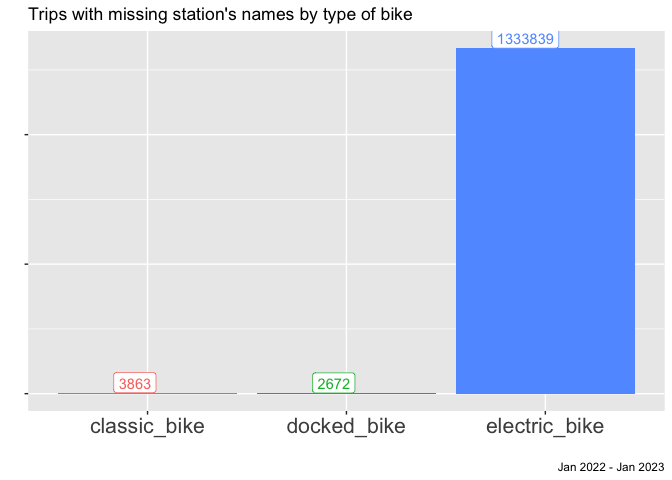
\includegraphics{CS_3_files/figure-latex/Missing stations name-1.pdf}

The reason could be a complete discharge of the batteries.

100 observations have negative trip duration.

\begin{Shaded}
\begin{Highlighting}[]
\NormalTok{raw\_df }\SpecialCharTok{\%\textgreater{}\%}
  \FunctionTok{filter}\NormalTok{(trip\_duration }\SpecialCharTok{\textless{}} \DecValTok{0}\NormalTok{) }\SpecialCharTok{\%\textgreater{}\%}
  \FunctionTok{group\_by}\NormalTok{(rideable\_type) }\SpecialCharTok{\%\textgreater{}\%}
  \FunctionTok{summarise}\NormalTok{(}\AttributeTok{sum=} \FunctionTok{n}\NormalTok{()) }\SpecialCharTok{\%\textgreater{}\%} 
  \FunctionTok{as\_flextable}\NormalTok{()}
\end{Highlighting}
\end{Shaded}

\begin{verbatim}
## Warning: fonts used in `flextable` are ignored because the `pdflatex` engine is
## used and not `xelatex` or `lualatex`. You can avoid this warning by using the
## `set_flextable_defaults(fonts_ignore=TRUE)` command or use a compatible engine
## by defining `latex_engine: xelatex` in the YAML header of the R Markdown
## document.
\end{verbatim}

\global\setlength{\Oldarrayrulewidth}{\arrayrulewidth}

\global\setlength{\Oldtabcolsep}{\tabcolsep}

\setlength{\tabcolsep}{0pt}

\renewcommand*{\arraystretch}{1.5}



\providecommand{\ascline}[3]{\noalign{\global\arrayrulewidth #1}\arrayrulecolor[HTML]{#2}\cline{#3}}

\begin{longtable}[c]{|p{1.20in}|p{0.75in}}



\ascline{1.5pt}{666666}{1-2}

\multicolumn{1}{>{\raggedright}m{\dimexpr 1.2in+0\tabcolsep}}{\textcolor[HTML]{000000}{\fontsize{11}{11}\selectfont{rideable\_type}}} & \multicolumn{1}{>{\raggedleft}m{\dimexpr 0.75in+0\tabcolsep}}{\textcolor[HTML]{000000}{\fontsize{11}{11}\selectfont{sum}}} \\





\multicolumn{1}{>{\raggedright}m{\dimexpr 1.2in+0\tabcolsep}}{\textcolor[HTML]{999999}{\fontsize{11}{11}\selectfont{character}}} & \multicolumn{1}{>{\raggedleft}m{\dimexpr 0.75in+0\tabcolsep}}{\textcolor[HTML]{999999}{\fontsize{11}{11}\selectfont{integer}}} \\

\ascline{1.5pt}{666666}{1-2}\endhead



\multicolumn{1}{>{\raggedright}m{\dimexpr 1.2in+0\tabcolsep}}{\textcolor[HTML]{000000}{\fontsize{11}{11}\selectfont{classic\_bike}}} & \multicolumn{1}{>{\raggedleft}m{\dimexpr 0.75in+0\tabcolsep}}{\textcolor[HTML]{000000}{\fontsize{11}{11}\selectfont{28}}} \\





\multicolumn{1}{>{\raggedright}m{\dimexpr 1.2in+0\tabcolsep}}{\textcolor[HTML]{000000}{\fontsize{11}{11}\selectfont{electric\_bike}}} & \multicolumn{1}{>{\raggedleft}m{\dimexpr 0.75in+0\tabcolsep}}{\textcolor[HTML]{000000}{\fontsize{11}{11}\selectfont{72}}} \\

\ascline{1.5pt}{666666}{1-2}



\end{longtable}



\arrayrulecolor[HTML]{000000}

\global\setlength{\arrayrulewidth}{\Oldarrayrulewidth}

\global\setlength{\tabcolsep}{\Oldtabcolsep}

\renewcommand*{\arraystretch}{1}

\hypertarget{the-data-is-not-clean}{%
\paragraph{The data is not clean}\label{the-data-is-not-clean}}

\begin{enumerate}
\def\labelenumi{\arabic{enumi}.}
\item
  \textbf{Domain integrity issue.} Standard deviation of
  \texttt{trip\_duration} is unreasonably high: ( 175 min, while mean
  =19 min). This clearly indicates the presence of extreme outliers.

  Some \texttt{started\_at} is greater than \texttt{ended\_at}. It means
  negative \texttt{trip\_duration} .
\item
  \textbf{Entity integrity issue.} 5985 trips (0.1\% of all trips) have
  no gps data at all. This concern we might take into account if we'll
  plan to investigate routes. Some observations at end stations include
  zeros.

  1.340.374 (23 \% of all trips) of data concerning station's names is
  empty. 99,5 \% among them are electric bikes.
\item
  \textbf{Referential integrity issue.} Station's naming is not
  consistent.

  The number of station identifiers is less than their names.\\
\end{enumerate}

\textbf{Solutions:}

\begin{enumerate}
\def\labelenumi{\arabic{enumi}.}
\item
  Exclude data with negative \texttt{trip\_duration} (100 observations)
\item
  Exclude data with too big \texttt{trip\_duration} (greater than 1499
  minutes, \textasciitilde25 hours) and with simultaneously empty
  \texttt{end\_station\_name}
\item
  Exclude classic bike's trips with missing station's names (3863
  observations)
\item
  Restore stations ID by geo data where possible. Maybe this won't screw
  the overall patterns but it's better to restore the missing data.
\end{enumerate}

\hypertarget{dropping-irrelevant-data}{%
\paragraph{Dropping irrelevant data}\label{dropping-irrelevant-data}}

The data has to be processed.\\

Let's take a look on distribution of ``strange'' observations\\
where
\texttt{trip\_duration\ \textgreater{}\ 1499\ \&\ rideable\_type\ !=\ "docked\_bike"}

\begin{Shaded}
\begin{Highlighting}[]
\NormalTok{raw\_df }\SpecialCharTok{\%\textgreater{}\%} 

  \FunctionTok{filter}\NormalTok{(rideable\_type }\SpecialCharTok{!=} \StringTok{"docked\_bike"}\NormalTok{) }\SpecialCharTok{\%\textgreater{}\%}
  \FunctionTok{filter}\NormalTok{(trip\_duration }\SpecialCharTok{\textgreater{}} \DecValTok{0}\NormalTok{) }\SpecialCharTok{\%\textgreater{}\%} 

  
  \FunctionTok{ggplot}\NormalTok{() }\SpecialCharTok{+}
  \FunctionTok{geom\_density}\NormalTok{(}\FunctionTok{aes}\NormalTok{(}\AttributeTok{x=}\NormalTok{trip\_duration)) }\SpecialCharTok{+}
  \FunctionTok{scale\_y\_log10}\NormalTok{() }\SpecialCharTok{+}
  \FunctionTok{geom\_segment}\NormalTok{(}\FunctionTok{aes}\NormalTok{(}\AttributeTok{x =} \FloatTok{1.35e3}\NormalTok{, }\AttributeTok{y =} \FloatTok{1e{-}2}\NormalTok{, }\AttributeTok{xend =} \FloatTok{1.49e3}\NormalTok{, }\AttributeTok{yend =} \FloatTok{3e{-}4}\NormalTok{),}\AttributeTok{color =} \StringTok{"red"}\NormalTok{,}
                 \AttributeTok{lineend =} \StringTok{"round"}\NormalTok{, }\AttributeTok{linejoin =} \StringTok{"mitre"}\NormalTok{,}
                  \AttributeTok{arrow =} \FunctionTok{arrow}\NormalTok{(}\AttributeTok{length =} \FunctionTok{unit}\NormalTok{(}\FloatTok{0.5}\NormalTok{, }\StringTok{"cm"}\NormalTok{)))}
\end{Highlighting}
\end{Shaded}

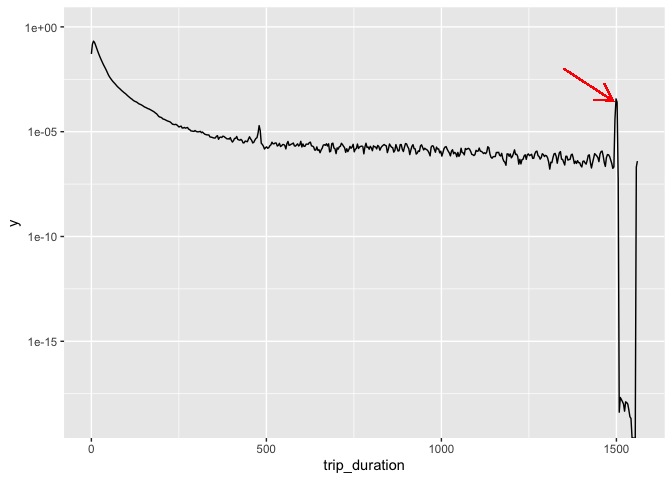
\includegraphics{CS_3_files/figure-latex/Dirty data distribution-1.pdf}

The surge at mark 25h(1500 minutes) \textbf{might be a service
notation}, e.g.~bikes that had been left out of parking stations, fully
discharged, defected or stolen bikes.

Finally, we will \textbf{consider a trip valid} if it satisfies the
following conditions:

\begin{enumerate}
\def\labelenumi{\arabic{enumi}.}
\item
  \texttt{rideable\_type\ !=\ "docked\_bike"} to exclude service
  observations.
\item
  \texttt{trip\_duration} \textgreater{} 1 minute (exclude any trips
  that were below 60 seconds in length (potentially false starts or
  users trying to re-dock a bike to ensure it was secure).
\item
  \texttt{trip\_duration} \textless{} 1499 minutes(25 hours).
  (\href{https://help.divvybikes.com/hc/en-us/articles/360033484791-What-if-I-keep-a-bike-out-too-long-}{NOTE:
  If you do not return a bike within a 24-hour period, you may be
  charged a lost or stolen bike fee of \$250 (plus tax}).
\item
  \texttt{end\_station\_name} is not empty
\end{enumerate}

\begin{Shaded}
\begin{Highlighting}[]
\NormalTok{raw\_df }\SpecialCharTok{\%\textgreater{}\%} 
  \FunctionTok{filter}\NormalTok{(rideable\_type }\SpecialCharTok{==} \StringTok{"docked\_bike"} \SpecialCharTok{|} \FunctionTok{is.na}\NormalTok{(end\_lat) }\SpecialCharTok{|}
\NormalTok{           trip\_duration }\SpecialCharTok{\textless{}} \DecValTok{1} \SpecialCharTok{|}\NormalTok{ trip\_duration }\SpecialCharTok{\textgreater{}} \DecValTok{1499}\NormalTok{ ) }\SpecialCharTok{\%\textgreater{}\%} 
  \FunctionTok{nrow}\NormalTok{()}
\end{Highlighting}
\end{Shaded}

\begin{verbatim}
## [1] 308332
\end{verbatim}

This assumption will exclude 308,332 (5.2 \%) observations from
``dirty'' data. This is acceptable.

We keep the source untouched and put valid data to \texttt{trip\_df} :

\begin{Shaded}
\begin{Highlighting}[]
\NormalTok{trip\_df }\OtherTok{\textless{}{-}}\NormalTok{ raw\_df }\SpecialCharTok{\%\textgreater{}\%} 
  \FunctionTok{filter}\NormalTok{(rideable\_type }\SpecialCharTok{!=} \StringTok{"docked\_bike"} \SpecialCharTok{\&} \SpecialCharTok{!}\FunctionTok{is.na}\NormalTok{(end\_lat)) }\SpecialCharTok{\%\textgreater{}\%} 
  \FunctionTok{filter}\NormalTok{(trip\_duration }\SpecialCharTok{\textgreater{}} \DecValTok{1} \SpecialCharTok{\&}
\NormalTok{           trip\_duration }\SpecialCharTok{\textless{}} \DecValTok{1499}\NormalTok{ ) }
\end{Highlighting}
\end{Shaded}

\hypertarget{restoring-missed-station-names}{%
\subsubsection{Restoring missed station
names}\label{restoring-missed-station-names}}

The logic:\\
1. Build a data frame (\texttt{stations\_df}) with all station's names
and appropriate geo data\\
2. Restore station's names according to the dictionary geo data.

Let's try.

\hypertarget{stations-names}{%
\paragraph{Station's names}\label{stations-names}}

To avoid duplicates we round the geo data to 4 decimals places (11 m
accuracy).

\begin{Shaded}
\begin{Highlighting}[]
\CommentTok{\# setting geo data accuracy (decimal places)}
\NormalTok{geo\_acc }\OtherTok{\textless{}{-}} \DecValTok{4}

\CommentTok{\# parcing end stations}
\NormalTok{stations\_df }\OtherTok{\textless{}{-}}\NormalTok{ trip\_df }\SpecialCharTok{\%\textgreater{}\%} 
    \FunctionTok{filter}\NormalTok{(end\_station\_name }\SpecialCharTok{!=} \StringTok{""} \SpecialCharTok{\&} 
\NormalTok{             (end\_lat }\SpecialCharTok{!=} \DecValTok{0} \SpecialCharTok{|} \SpecialCharTok{!}\FunctionTok{is.na}\NormalTok{(end\_lat) ) ) }\SpecialCharTok{\%\textgreater{}\%} 
  \FunctionTok{group\_by}\NormalTok{(end\_station\_name) }\SpecialCharTok{\%\textgreater{}\%} 

  \CommentTok{\# we use means here to increase geo data accuracy of stations}
  \FunctionTok{summarise}\NormalTok{(}\AttributeTok{latit =} \FunctionTok{mean}\NormalTok{(end\_lat), }
            \AttributeTok{lngit =} \FunctionTok{mean}\NormalTok{(end\_lng)) }\SpecialCharTok{\%\textgreater{}\%} 
  \FunctionTok{unique}\NormalTok{()}

\CommentTok{\# all columns with postfix \textquotesingle{}2\textquotesingle{} at the end will serve later as joining instances }
\NormalTok{stations\_df[,}\StringTok{"end\_lat2"}\NormalTok{] }\OtherTok{=} \FunctionTok{round}\NormalTok{(stations\_df}\SpecialCharTok{$}\NormalTok{latit,geo\_acc)}
\NormalTok{stations\_df[,}\StringTok{"end\_lng2"}\NormalTok{] }\OtherTok{=} \FunctionTok{round}\NormalTok{(stations\_df}\SpecialCharTok{$}\NormalTok{lngit,geo\_acc)}

\CommentTok{\# adding station IDs}
\NormalTok{stations\_df }\OtherTok{\textless{}{-}}
  \FunctionTok{left\_join}\NormalTok{(stations\_df, trip\_df, }\AttributeTok{by =} \FunctionTok{c}\NormalTok{(}\StringTok{"end\_station\_name"}\NormalTok{), }\AttributeTok{multiple =} \StringTok{"first"}\NormalTok{) }\SpecialCharTok{\%\textgreater{}\%} 
  \FunctionTok{select}\NormalTok{(}\StringTok{"end\_station\_id"}\NormalTok{,}
         \StringTok{"end\_station\_name"}\NormalTok{,}
         \StringTok{"latit"}\NormalTok{,}
         \StringTok{"lngit"}\NormalTok{,}
         \StringTok{"end\_lat2"}\NormalTok{,}
         \StringTok{"end\_lng2"}\NormalTok{)}
\CommentTok{\# renaming}
\NormalTok{stations\_df }\OtherTok{\textless{}{-}} 
  \FunctionTok{rename}\NormalTok{(stations\_df, }\FunctionTok{all\_of}\NormalTok{( }\FunctionTok{c}\NormalTok{(}\AttributeTok{station\_name =} \StringTok{"end\_station\_name"}\NormalTok{, }
                                \AttributeTok{station\_id =}  \StringTok{"end\_station\_id"}\NormalTok{)) )}


\CommentTok{\# parcing start stations}
\CommentTok{\# stations\_df2 {-} start\_station data frame}
\NormalTok{stations\_df2 }\OtherTok{\textless{}{-}}\NormalTok{ trip\_df }\SpecialCharTok{\%\textgreater{}\%} 
    \FunctionTok{filter}\NormalTok{(start\_station\_name }\SpecialCharTok{!=} \StringTok{""}\NormalTok{ ) }\SpecialCharTok{\%\textgreater{}\%} 
  \FunctionTok{group\_by}\NormalTok{(start\_station\_name) }\SpecialCharTok{\%\textgreater{}\%} 
  \CommentTok{\# all columns with \textquotesingle{}2\textquotesingle{} at the end will serve later as joining instances }
  \CommentTok{\# we use means here to increase geo data accuracy}
  \FunctionTok{summarise}\NormalTok{(}\AttributeTok{latit =} \FunctionTok{mean}\NormalTok{(start\_lat), }
            \AttributeTok{lngit =} \FunctionTok{mean}\NormalTok{(start\_lng) ) }\SpecialCharTok{\%\textgreater{}\%} 
  \FunctionTok{unique}\NormalTok{()}

\CommentTok{\# all columns with postfix \textquotesingle{}2\textquotesingle{} at the end will serve later as joining instances }
\NormalTok{stations\_df2[,}\StringTok{"end\_lat2"}\NormalTok{] }\OtherTok{=} \FunctionTok{round}\NormalTok{(stations\_df2}\SpecialCharTok{$}\NormalTok{latit,geo\_acc)}
\NormalTok{stations\_df2[,}\StringTok{"end\_lng2"}\NormalTok{] }\OtherTok{=} \FunctionTok{round}\NormalTok{(stations\_df2}\SpecialCharTok{$}\NormalTok{lngit,geo\_acc)}


\CommentTok{\# adding station IDs}
\NormalTok{stations\_df2 }\OtherTok{\textless{}{-}}
  \FunctionTok{left\_join}\NormalTok{(stations\_df2, trip\_df, }\AttributeTok{by =} \FunctionTok{c}\NormalTok{(}\StringTok{"start\_station\_name"}\NormalTok{), }\AttributeTok{multiple =} \StringTok{"first"}\NormalTok{) }\SpecialCharTok{\%\textgreater{}\%} 
  \FunctionTok{select}\NormalTok{(}\StringTok{"start\_station\_id"}\NormalTok{,}
         \StringTok{"start\_station\_name"}\NormalTok{,}
         \StringTok{"latit"}\NormalTok{,}
         \StringTok{"lngit"}\NormalTok{,         }
         \StringTok{"end\_lat2"}\NormalTok{,}
         \StringTok{"end\_lng2"}\NormalTok{)}
\CommentTok{\# renaming}
\NormalTok{stations\_df2 }\OtherTok{\textless{}{-}} 
  \FunctionTok{rename}\NormalTok{(stations\_df2, }\FunctionTok{all\_of}\NormalTok{( }\FunctionTok{c}\NormalTok{(}\AttributeTok{station\_name =} \StringTok{"start\_station\_name"}\NormalTok{, }
                                \AttributeTok{station\_id =}  \StringTok{"start\_station\_id"}\NormalTok{)) )}

\NormalTok{stations\_df }\OtherTok{\textless{}{-}}
  \FunctionTok{bind\_rows}\NormalTok{(stations\_df, stations\_df2) }\SpecialCharTok{\%\textgreater{}\%} 
\NormalTok{  dplyr}\SpecialCharTok{::}\FunctionTok{distinct}\NormalTok{(station\_name, }\AttributeTok{.keep\_all =} \ConstantTok{TRUE}\NormalTok{) }
\end{Highlighting}
\end{Shaded}

\hypertarget{restoring-stations-names}{%
\paragraph{Restoring stations names}\label{restoring-stations-names}}

\hypertarget{restoring-end_station_name-and-end_station_id.}{%
\subparagraph{\texorpdfstring{Restoring \texttt{end\_station\_name} and
\texttt{end\_station\_id}.}{Restoring end\_station\_name and end\_station\_id.}}\label{restoring-end_station_name-and-end_station_id.}}

\begin{Shaded}
\begin{Highlighting}[]
\CommentTok{\# service columns with rounded geo data}
\NormalTok{trip\_df[,}\StringTok{"end\_lat2"}\NormalTok{] }\OtherTok{\textless{}{-}} \FunctionTok{round}\NormalTok{(trip\_df}\SpecialCharTok{$}\NormalTok{end\_lat,geo\_acc)}
\NormalTok{trip\_df[,}\StringTok{"end\_lng2"}\NormalTok{] }\OtherTok{\textless{}{-}} \FunctionTok{round}\NormalTok{(trip\_df}\SpecialCharTok{$}\NormalTok{end\_lng,geo\_acc)}
\NormalTok{trip\_df[,}\StringTok{"restored"}\NormalTok{] }\OtherTok{\textless{}{-}} \ConstantTok{NA}

\NormalTok{trip\_df }\OtherTok{\textless{}{-}} 
  \FunctionTok{left\_join}\NormalTok{(trip\_df, stations\_df, }\AttributeTok{by =} \FunctionTok{c}\NormalTok{(}\StringTok{"end\_lat2"}\NormalTok{,}\StringTok{"end\_lng2"}\NormalTok{), }\AttributeTok{multiple =} \StringTok{\textquotesingle{}first\textquotesingle{}}\NormalTok{) }

\CommentTok{\# logging restoration}
\NormalTok{trip\_df}\SpecialCharTok{$}\NormalTok{restored }\OtherTok{=} 
  \FunctionTok{ifelse}\NormalTok{(trip\_df}\SpecialCharTok{$}\NormalTok{end\_station\_name }\SpecialCharTok{==} \StringTok{""} \SpecialCharTok{\&} \SpecialCharTok{!}\FunctionTok{is.na}\NormalTok{(trip\_df}\SpecialCharTok{$}\NormalTok{station\_name),}
         \StringTok{"end\_station\_name"}\NormalTok{,}
         \FunctionTok{ifelse}\NormalTok{(trip\_df}\SpecialCharTok{$}\NormalTok{end\_station\_id }\SpecialCharTok{==} \StringTok{""} \SpecialCharTok{\&} \SpecialCharTok{!}\FunctionTok{is.na}\NormalTok{(trip\_df}\SpecialCharTok{$}\NormalTok{station\_id),}
                \StringTok{"end\_station\_id"}\NormalTok{, }\ConstantTok{NA}\NormalTok{)}
\NormalTok{  )}
\CommentTok{\# adding end\_station\_name}
\NormalTok{trip\_df}\SpecialCharTok{$}\NormalTok{end\_station\_name }\OtherTok{=} 
  \FunctionTok{ifelse}\NormalTok{(trip\_df}\SpecialCharTok{$}\NormalTok{end\_station\_name }\SpecialCharTok{==} \StringTok{""}\SpecialCharTok{\&} \SpecialCharTok{!}\FunctionTok{is.na}\NormalTok{(trip\_df}\SpecialCharTok{$}\NormalTok{station\_name),}
\NormalTok{         trip\_df}\SpecialCharTok{$}\NormalTok{station\_name,}
\NormalTok{         trip\_df}\SpecialCharTok{$}\NormalTok{end\_station\_name) }
\CommentTok{\# adding end\_station\_id}
\NormalTok{trip\_df}\SpecialCharTok{$}\NormalTok{end\_station\_id }\OtherTok{=} 
  \FunctionTok{ifelse}\NormalTok{(trip\_df}\SpecialCharTok{$}\NormalTok{end\_station\_id }\SpecialCharTok{==} \StringTok{""}\SpecialCharTok{\&} \SpecialCharTok{!}\FunctionTok{is.na}\NormalTok{(trip\_df}\SpecialCharTok{$}\NormalTok{station\_id),}
\NormalTok{         trip\_df}\SpecialCharTok{$}\NormalTok{station\_id,}
\NormalTok{         trip\_df}\SpecialCharTok{$}\NormalTok{end\_station\_id) }

\CommentTok{\# dropping service joining columns}
\NormalTok{trip\_df }\OtherTok{\textless{}{-}} \FunctionTok{within}\NormalTok{(trip\_df, }\FunctionTok{rm}\NormalTok{(}\StringTok{"end\_lat2"}\NormalTok{,}
                                        \StringTok{"end\_lng2"}\NormalTok{,}
                                        \StringTok{"station\_id"}\NormalTok{,}
                                        \StringTok{"station\_name"}\NormalTok{ ))}
\end{Highlighting}
\end{Shaded}

\hypertarget{restoring-start_station_name-and-start_station_id.}{%
\subparagraph{\texorpdfstring{Restoring \texttt{start\_station\_name}
and
\texttt{start\_station\_id}.}{Restoring start\_station\_name and start\_station\_id.}}\label{restoring-start_station_name-and-start_station_id.}}

\begin{Shaded}
\begin{Highlighting}[]
\NormalTok{trip\_df[,}\StringTok{"start\_lat2"}\NormalTok{] }\OtherTok{\textless{}{-}} \FunctionTok{round}\NormalTok{(trip\_df}\SpecialCharTok{$}\NormalTok{start\_lat,geo\_acc)}
\NormalTok{trip\_df[,}\StringTok{"start\_lng2"}\NormalTok{] }\OtherTok{\textless{}{-}} \FunctionTok{round}\NormalTok{(trip\_df}\SpecialCharTok{$}\NormalTok{start\_lng,geo\_acc)}

\NormalTok{stations\_df }\OtherTok{\textless{}{-}} 
  \FunctionTok{rename}\NormalTok{(stations\_df, }\FunctionTok{all\_of}\NormalTok{( }\FunctionTok{c}\NormalTok{(}\AttributeTok{start\_lat2 =} \StringTok{"end\_lat2"}\NormalTok{, }
                                \AttributeTok{start\_lng2 =}  \StringTok{"end\_lng2"}\NormalTok{)) )}

\NormalTok{trip\_df }\OtherTok{\textless{}{-}} 
  \FunctionTok{left\_join}\NormalTok{(trip\_df, stations\_df, }\AttributeTok{by =} \FunctionTok{c}\NormalTok{(}\StringTok{"start\_lat2"}\NormalTok{,}\StringTok{"start\_lng2"}\NormalTok{), }\AttributeTok{multiple =} \StringTok{\textquotesingle{}first\textquotesingle{}}\NormalTok{) }
\CommentTok{\# logging restoration}
\NormalTok{trip\_df}\SpecialCharTok{$}\NormalTok{restored }\OtherTok{=} 
  \FunctionTok{ifelse}\NormalTok{(trip\_df}\SpecialCharTok{$}\NormalTok{start\_station\_name }\SpecialCharTok{==} \StringTok{""} \SpecialCharTok{\&} \SpecialCharTok{!}\FunctionTok{is.na}\NormalTok{(trip\_df}\SpecialCharTok{$}\NormalTok{station\_name),}
         \StringTok{"start\_station\_name"}\NormalTok{,}
         \FunctionTok{ifelse}\NormalTok{(trip\_df}\SpecialCharTok{$}\NormalTok{start\_station\_id }\SpecialCharTok{==} \StringTok{""} \SpecialCharTok{\&} \SpecialCharTok{!}\FunctionTok{is.na}\NormalTok{(trip\_df}\SpecialCharTok{$}\NormalTok{station\_id),}
                \StringTok{"start\_station\_id"}\NormalTok{, }\ConstantTok{NA}\NormalTok{)}
\NormalTok{  )}

\CommentTok{\# adding start\_station\_name}
\NormalTok{trip\_df}\SpecialCharTok{$}\NormalTok{start\_station\_name }\OtherTok{=} 
  \FunctionTok{ifelse}\NormalTok{(trip\_df}\SpecialCharTok{$}\NormalTok{start\_station\_name }\SpecialCharTok{==} \StringTok{""} \SpecialCharTok{\&} \SpecialCharTok{!}\FunctionTok{is.na}\NormalTok{(trip\_df}\SpecialCharTok{$}\NormalTok{station\_name),}
\NormalTok{         trip\_df}\SpecialCharTok{$}\NormalTok{station\_name,}
\NormalTok{         trip\_df}\SpecialCharTok{$}\NormalTok{start\_station\_name) }
\CommentTok{\# adding start\_station\_id}
\NormalTok{trip\_df}\SpecialCharTok{$}\NormalTok{start\_station\_id }\OtherTok{=} 
  \FunctionTok{ifelse}\NormalTok{(trip\_df}\SpecialCharTok{$}\NormalTok{start\_station\_id }\SpecialCharTok{==} \StringTok{""} \SpecialCharTok{\&} \SpecialCharTok{!}\FunctionTok{is.na}\NormalTok{(trip\_df}\SpecialCharTok{$}\NormalTok{station\_id),}
\NormalTok{         trip\_df}\SpecialCharTok{$}\NormalTok{station\_id,}
\NormalTok{         trip\_df}\SpecialCharTok{$}\NormalTok{start\_station\_id) }

\CommentTok{\# dropping joining columns}
\NormalTok{trip\_df }\OtherTok{\textless{}{-}} \FunctionTok{within}\NormalTok{(trip\_df, }\FunctionTok{rm}\NormalTok{(}
                                  \StringTok{"start\_lat2"}\NormalTok{,}
                                  \StringTok{"start\_lng2"}\NormalTok{,}
                                  \StringTok{"station\_id"}\NormalTok{,}
                                  \StringTok{"station\_name"}\NormalTok{,}
                                  \StringTok{"latit.x"}\NormalTok{,}
                                  \StringTok{"lngit.x"}\NormalTok{,}
                                  \StringTok{"latit.y"}\NormalTok{,}
                                  \StringTok{"lngit.y"}\NormalTok{))}
\FunctionTok{nrow}\NormalTok{(}\FunctionTok{filter}\NormalTok{(trip\_df, }\SpecialCharTok{!}\FunctionTok{is.na}\NormalTok{(restored) ) )}
\end{Highlighting}
\end{Shaded}

\begin{verbatim}
## [1] 312438
\end{verbatim}

We've managed to restore station's names within 312,438 (291,850)
observations.\\

Converting cleaned data frame to tibble:

\begin{Shaded}
\begin{Highlighting}[]
\NormalTok{df }\OtherTok{\textless{}{-}} \FunctionTok{as\_tibble}\NormalTok{(trip\_df) }
\end{Highlighting}
\end{Shaded}

Adding a trip the day of the week :

\begin{Shaded}
\begin{Highlighting}[]
\NormalTok{df[, }\StringTok{"weekday"}\NormalTok{] }\OtherTok{\textless{}{-}} \FunctionTok{wday}\NormalTok{(df}\SpecialCharTok{$}\NormalTok{started\_at, }\AttributeTok{label =} \ConstantTok{TRUE}\NormalTok{)}
\end{Highlighting}
\end{Shaded}

\hypertarget{analyse}{%
\subsection{4. ANALYSE}\label{analyse}}

\hypertarget{assumptions-and-constraints}{%
\paragraph{Assumptions and
constraints}\label{assumptions-and-constraints}}

Let's take a look at distribution of trips over data set:

\begin{Shaded}
\begin{Highlighting}[]
\NormalTok{df }\SpecialCharTok{\%\textgreater{}\%} 
  \FunctionTok{ggplot}\NormalTok{(}\FunctionTok{aes}\NormalTok{(}\AttributeTok{x=}\NormalTok{trip\_duration, }\AttributeTok{y=}\NormalTok{ member\_casual)) }\SpecialCharTok{+}
  \FunctionTok{geom\_boxplot}\NormalTok{( }\AttributeTok{outlier.colour =} \StringTok{"red"}\NormalTok{,}
                \AttributeTok{outlier.stroke =} \DecValTok{0}\NormalTok{, }
                \AttributeTok{outlier.alpha =} \FloatTok{0.1}\NormalTok{,}
                \AttributeTok{varwidth =} \ConstantTok{FALSE}\NormalTok{) }\SpecialCharTok{+}
  \FunctionTok{scale\_x\_log10}\NormalTok{()}
\end{Highlighting}
\end{Shaded}

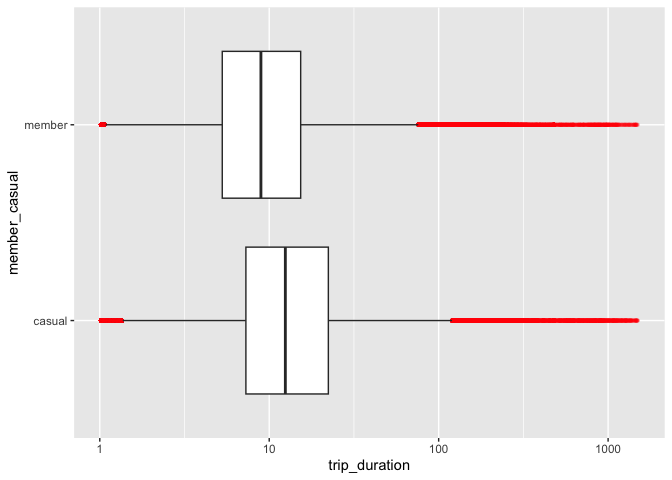
\includegraphics{CS_3_files/figure-latex/distribution of trips over data set-1.pdf}

There are too many outliers that might skew overall statistics.\\

We constrain data with :

\begin{itemize}
\tightlist
\item
  the upper limit to \texttt{mean\ +\ 5sigma} = 142 minutes
\end{itemize}

\begin{Shaded}
\begin{Highlighting}[]
\NormalTok{(trip\_limit }\OtherTok{\textless{}{-}} \FunctionTok{mean}\NormalTok{(df}\SpecialCharTok{$}\NormalTok{trip\_duration) }\SpecialCharTok{+} \DecValTok{5}\SpecialCharTok{*} \FunctionTok{sd}\NormalTok{(df}\SpecialCharTok{$}\NormalTok{trip\_duration) )}
\end{Highlighting}
\end{Shaded}

\begin{verbatim}
## [1] 142.4059
\end{verbatim}

It removes only 17.837 rows (0.3 \% of all trips). So our conclusions
will be based on 99.7 \% of ``clean'' data.

\begin{Shaded}
\begin{Highlighting}[]
\FunctionTok{count}\NormalTok{(}\FunctionTok{filter}\NormalTok{(df, trip\_duration }\SpecialCharTok{\textgreater{}}\NormalTok{ trip\_limit))}
\end{Highlighting}
\end{Shaded}

\begin{verbatim}
## # A tibble: 1 x 1
##       n
##   <int>
## 1 17837
\end{verbatim}

\begin{Shaded}
\begin{Highlighting}[]
\FunctionTok{filter}\NormalTok{(df, trip\_duration }\SpecialCharTok{\textless{}}\NormalTok{ trip\_limit) }\OtherTok{{-}\textgreater{}}\NormalTok{ df}
\end{Highlighting}
\end{Shaded}

\hypertarget{descriptive-statistics.-trip-durations}{%
\subsubsection{Descriptive statistics. Trip
durations}\label{descriptive-statistics.-trip-durations}}

\hypertarget{average-duration-of-one-trip-throughout-a-year}{%
\paragraph{Average duration of one trip throughout a
year}\label{average-duration-of-one-trip-throughout-a-year}}

\begin{Shaded}
\begin{Highlighting}[]
\NormalTok{df }\SpecialCharTok{\%\textgreater{}\%} 
  \FunctionTok{group\_by}\NormalTok{(member\_casual, weekday) }\SpecialCharTok{\%\textgreater{}\%} 
  \FunctionTok{summarise}\NormalTok{(}\AttributeTok{ride\_mean =} \FunctionTok{round}\NormalTok{(}\FunctionTok{mean}\NormalTok{(trip\_duration),}\DecValTok{1}\NormalTok{))  }\SpecialCharTok{\%\textgreater{}\%} 
  \CommentTok{\# summarise(ride\_mean = round(mean(trip\_duration),1))  \%\textgreater{}\%   }
  \FunctionTok{ggplot}\NormalTok{() }\SpecialCharTok{+}
  \FunctionTok{geom\_col}\NormalTok{(}\FunctionTok{aes}\NormalTok{(}\AttributeTok{y =}\NormalTok{ ride\_mean, }\AttributeTok{x =}\NormalTok{ weekday, }\AttributeTok{fill =}\NormalTok{ member\_casual ),}
           \AttributeTok{position =} \StringTok{"dodge"}\NormalTok{) }\SpecialCharTok{+} \CommentTok{\#, show.legend = FALSE, , alpha = 0.8}
  \FunctionTok{labs}\NormalTok{(}\AttributeTok{title =} \StringTok{"Average duration of one trip by day of the week"}\NormalTok{,}
       \AttributeTok{caption =}\NormalTok{ report\_caption,}
       \AttributeTok{x =}\StringTok{""}\NormalTok{, }\AttributeTok{y=} \StringTok{"minutes"}\NormalTok{,}
       \AttributeTok{fill=}\StringTok{\textquotesingle{}Type of rider\textquotesingle{}}\NormalTok{) }\SpecialCharTok{+}
  \FunctionTok{scale\_y\_continuous}\NormalTok{(}\AttributeTok{labels =} \FunctionTok{label\_comma}\NormalTok{()) }\SpecialCharTok{+}
\FunctionTok{geom\_label}\NormalTok{(}\FunctionTok{aes}\NormalTok{(}\AttributeTok{y =}\NormalTok{ ride\_mean, }\AttributeTok{x =}\NormalTok{ weekday, }\AttributeTok{label =}\NormalTok{ ride\_mean,}
               \AttributeTok{color =}\NormalTok{ member\_casual), }\AttributeTok{hjust =}\FloatTok{0.8}\NormalTok{, }\AttributeTok{vjust =} \FloatTok{1.5}\NormalTok{, }\AttributeTok{show.legend =} \ConstantTok{FALSE}\NormalTok{)}
\end{Highlighting}
\end{Shaded}

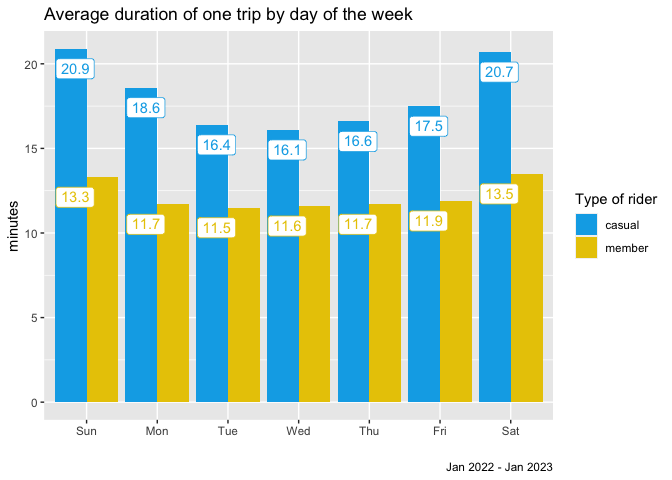
\includegraphics{CS_3_files/figure-latex/Average duration of one trip-1.pdf}

\begin{Shaded}
\begin{Highlighting}[]
\NormalTok{df }\SpecialCharTok{\%\textgreater{}\%} 
  \FunctionTok{group\_by}\NormalTok{(member\_casual) }\SpecialCharTok{\%\textgreater{}\%} 
  \FunctionTok{summarise}\NormalTok{(}\AttributeTok{ride\_mean =} \FunctionTok{round}\NormalTok{(}\FunctionTok{mean}\NormalTok{(trip\_duration),}\DecValTok{1}\NormalTok{) ) }\SpecialCharTok{\%\textgreater{}\%} 
  \FunctionTok{as\_flextable}\NormalTok{()  }\SpecialCharTok{\%\textgreater{}\%} 
\FunctionTok{set\_caption}\NormalTok{(}\FunctionTok{paste}\NormalTok{(}\StringTok{"Trip average duration."}\NormalTok{, report\_caption)) }\SpecialCharTok{\%\textgreater{}\%} \FunctionTok{delete\_part}\NormalTok{(}\StringTok{"header"}\NormalTok{)}
\end{Highlighting}
\end{Shaded}

\begin{verbatim}
## Warning: fonts used in `flextable` are ignored because the `pdflatex` engine is
## used and not `xelatex` or `lualatex`. You can avoid this warning by using the
## `set_flextable_defaults(fonts_ignore=TRUE)` command or use a compatible engine
## by defining `latex_engine: xelatex` in the YAML header of the R Markdown
## document.
\end{verbatim}

\global\setlength{\Oldarrayrulewidth}{\arrayrulewidth}

\global\setlength{\Oldtabcolsep}{\tabcolsep}

\setlength{\tabcolsep}{0pt}

\renewcommand*{\arraystretch}{1.5}



\providecommand{\ascline}[3]{\noalign{\global\arrayrulewidth #1}\arrayrulecolor[HTML]{#2}\cline{#3}}

\begin{longtable}[c]{|p{1.37in}|p{1.01in}}

\caption{Trip\ average\ duration.\ Jan\ 2022\ -\ Jan\ 2023}\\



\multicolumn{1}{>{\raggedright}m{\dimexpr 1.37in+0\tabcolsep}}{\textcolor[HTML]{000000}{\fontsize{11}{11}\selectfont{casual}}} & \multicolumn{1}{>{\raggedleft}m{\dimexpr 1.01in+0\tabcolsep}}{\textcolor[HTML]{000000}{\fontsize{11}{11}\selectfont{18.4}}} \\





\multicolumn{1}{>{\raggedright}m{\dimexpr 1.37in+0\tabcolsep}}{\textcolor[HTML]{000000}{\fontsize{11}{11}\selectfont{member}}} & \multicolumn{1}{>{\raggedleft}m{\dimexpr 1.01in+0\tabcolsep}}{\textcolor[HTML]{000000}{\fontsize{11}{11}\selectfont{12.1}}} \\

\ascline{1.5pt}{666666}{1-2}



\end{longtable}



\arrayrulecolor[HTML]{000000}

\global\setlength{\arrayrulewidth}{\Oldarrayrulewidth}

\global\setlength{\tabcolsep}{\Oldtabcolsep}

\renewcommand*{\arraystretch}{1}

\begin{Shaded}
\begin{Highlighting}[]
\CommentTok{\# df \%\textgreater{}\% }
\CommentTok{\#   crosstable(c(" "= trip\_duration), by=c(rider=member\_casual), funs=c("Average duration"= mean),  showNA="no", percent\_digits=0, percent\_pattern="\{n\} (\{p\_col\})") \%\textgreater{}\% }
\CommentTok{\#   as\_flextable(compact=TRUE, keep\_id=FALSE)  \%\textgreater{}\% }
\CommentTok{\#   set\_caption(paste("Trip average duration.", report\_caption))  \#\%\textgreater{}\% delete\_part("header")}
\end{Highlighting}
\end{Shaded}

Insights:

\begin{itemize}
\item
  Average duration of \textbf{casual riders is significantly higher} (+
  51 \%)
\item
  Trips on \textbf{Wednesdays} are 17 \% shorter than on weekends among
  all customers.
\end{itemize}

\hypertarget{the-maximum-ride-duration}{%
\paragraph{The maximum ride duration}\label{the-maximum-ride-duration}}

Finding the maximum ride duration we assume:

\begin{enumerate}
\def\labelenumi{\arabic{enumi}.}
\item
  Bike is not docked
\item
  Start and end stations are defined
\item
  We'll look up through the source data
\end{enumerate}

\begin{Shaded}
\begin{Highlighting}[]
\NormalTok{raw\_df  }\SpecialCharTok{\%\textgreater{}\%} 
  \FunctionTok{filter}\NormalTok{(rideable\_type }\SpecialCharTok{!=} \StringTok{"docked\_bike"}\NormalTok{) }\SpecialCharTok{\%\textgreater{}\%}
  \FunctionTok{filter}\NormalTok{(start\_station\_name }\SpecialCharTok{!=}\StringTok{""} \SpecialCharTok{\&}\NormalTok{ end\_station\_name }\SpecialCharTok{!=} \StringTok{""}\NormalTok{) }\SpecialCharTok{\%\textgreater{}\%} 
  \CommentTok{\# group\_by(rideable\_type) \%\textgreater{}\% }
  \CommentTok{\# summarise(max=as.duration(max(ended\_at {-} started\_at))) \%\textgreater{}\% }
  \FunctionTok{crosstable}\NormalTok{(}\FunctionTok{c}\NormalTok{(}\StringTok{" "}\OtherTok{=}\NormalTok{ trip\_duration), }\AttributeTok{by=}\FunctionTok{c}\NormalTok{(}\AttributeTok{bycicle =}\NormalTok{ rideable\_type), }\AttributeTok{funs=}\FunctionTok{c}\NormalTok{(}\StringTok{"Max trip in minutes"}\OtherTok{=}\NormalTok{ max),  }\AttributeTok{showNA=}\StringTok{"no"}\NormalTok{, }\AttributeTok{percent\_digits=}\DecValTok{0}\NormalTok{, }\AttributeTok{percent\_pattern=}\StringTok{"\{n\} (\{p\_col\})"}\NormalTok{) }\SpecialCharTok{\%\textgreater{}\%} 
  \FunctionTok{as\_flextable}\NormalTok{(}\AttributeTok{compact=}\ConstantTok{TRUE}\NormalTok{, }\AttributeTok{keep\_id=}\ConstantTok{FALSE}\NormalTok{)  }\SpecialCharTok{\%\textgreater{}\%} 
  \FunctionTok{set\_caption}\NormalTok{(}\FunctionTok{paste}\NormalTok{(}\StringTok{"The maximum ride duration."}\NormalTok{, report\_caption))}
\end{Highlighting}
\end{Shaded}

\begin{verbatim}
## Warning: fonts used in `flextable` are ignored because the `pdflatex` engine is
## used and not `xelatex` or `lualatex`. You can avoid this warning by using the
## `set_flextable_defaults(fonts_ignore=TRUE)` command or use a compatible engine
## by defining `latex_engine: xelatex` in the YAML header of the R Markdown
## document.
\end{verbatim}

\global\setlength{\Oldarrayrulewidth}{\arrayrulewidth}

\global\setlength{\Oldtabcolsep}{\tabcolsep}

\setlength{\tabcolsep}{0pt}

\renewcommand*{\arraystretch}{1.5}



\providecommand{\ascline}[3]{\noalign{\global\arrayrulewidth #1}\arrayrulecolor[HTML]{#2}\cline{#3}}

\begin{longtable}[c]{|p{1.94in}|p{1.19in}|p{1.21in}}

\caption{The\ maximum\ ride\ duration.\ Jan\ 2022\ -\ Jan\ 2023}\\

\ascline{1.5pt}{000000}{1-3}

\multicolumn{1}{>{\centering}m{\dimexpr 1.94in+0\tabcolsep}}{} & \multicolumn{2}{>{\centering}m{\dimexpr 2.4in+2\tabcolsep}}{\textcolor[HTML]{000000}{\fontsize{11}{11}\selectfont{\textbf{bycicle}}}} \\

\ascline{1pt}{000000}{2-3}



\multicolumn{1}{>{\centering}m{\dimexpr 1.94in+0\tabcolsep}}{\multirow[c]{-2}{*}{\parbox{1.94in}{\textcolor[HTML]{000000}{\fontsize{11}{11}\selectfont{\textbf{}}}}}} & \multicolumn{1}{>{\centering}m{\dimexpr 1.19in+0\tabcolsep}}{\textcolor[HTML]{000000}{\fontsize{11}{11}\selectfont{\textbf{classic\_bike}}}} & \multicolumn{1}{>{\centering}m{\dimexpr 1.21in+0\tabcolsep}}{\textcolor[HTML]{000000}{\fontsize{11}{11}\selectfont{\textbf{electric\_bike}}}} \\

\ascline{1.5pt}{000000}{1-3}\endhead



\multicolumn{1}{>{\raggedright}m{\dimexpr 1.94in+0\tabcolsep}}{\textcolor[HTML]{000000}{\fontsize{11}{11}\selectfont{\textbf{\ }}}} & \multicolumn{1}{>{\raggedright}m{\dimexpr 1.19in+0\tabcolsep}}{\textcolor[HTML]{000000}{\fontsize{11}{11}\selectfont{\textbf{}}}} & \multicolumn{1}{>{\raggedright}m{\dimexpr 1.21in+0\tabcolsep}}{\textcolor[HTML]{000000}{\fontsize{11}{11}\selectfont{}}} \\





\multicolumn{1}{>{\raggedright}m{\dimexpr 1.94in+0\tabcolsep}}{\textcolor[HTML]{000000}{\fontsize{11}{11}\selectfont{Max\ trip\ in\ minutes}}} & \multicolumn{1}{>{\raggedright}m{\dimexpr 1.19in+0\tabcolsep}}{\textcolor[HTML]{000000}{\fontsize{11}{11}\selectfont{1499.4}}} & \multicolumn{1}{>{\raggedright}m{\dimexpr 1.21in+0\tabcolsep}}{\textcolor[HTML]{000000}{\fontsize{11}{11}\selectfont{480.0}}} \\

\ascline{1.5pt}{666666}{1-3}



\end{longtable}



\arrayrulecolor[HTML]{000000}

\global\setlength{\arrayrulewidth}{\Oldarrayrulewidth}

\global\setlength{\tabcolsep}{\Oldtabcolsep}

\renewcommand*{\arraystretch}{1}

\begin{Shaded}
\begin{Highlighting}[]
\NormalTok{raw\_df  }\SpecialCharTok{\%\textgreater{}\%} 
  \FunctionTok{filter}\NormalTok{(rideable\_type }\SpecialCharTok{!=} \StringTok{"docked\_bike"}\NormalTok{) }\SpecialCharTok{\%\textgreater{}\%}
  \FunctionTok{filter}\NormalTok{(start\_station\_name }\SpecialCharTok{!=}\StringTok{""} \SpecialCharTok{\&}\NormalTok{ end\_station\_name }\SpecialCharTok{!=} \StringTok{""} \SpecialCharTok{\&}
           \SpecialCharTok{!}\FunctionTok{is.na}\NormalTok{(end\_lat)) }\SpecialCharTok{\%\textgreater{}\%} 
  \FunctionTok{group\_by}\NormalTok{(rideable\_type) }\SpecialCharTok{\%\textgreater{}\%} 
  \FunctionTok{summarise}\NormalTok{(}\AttributeTok{max=}\FunctionTok{as.duration}\NormalTok{(}\FunctionTok{max}\NormalTok{(ended\_at }\SpecialCharTok{{-}}\NormalTok{ started\_at))) }\SpecialCharTok{\%\textgreater{}\%}

  \FunctionTok{ggplot}\NormalTok{() }\SpecialCharTok{+} 
  \FunctionTok{geom\_col}\NormalTok{(}\FunctionTok{aes}\NormalTok{(}\AttributeTok{y =}\NormalTok{ max, }\AttributeTok{x =}\NormalTok{ rideable\_type, }\AttributeTok{fill =}\NormalTok{ rideable\_type ),}
           \AttributeTok{show.legend =} \ConstantTok{FALSE}\NormalTok{) }\SpecialCharTok{+}
  \FunctionTok{geom\_label}\NormalTok{(}\FunctionTok{aes}\NormalTok{(}\AttributeTok{y =}\NormalTok{ max, }\AttributeTok{x =}\NormalTok{ rideable\_type, }
                 \AttributeTok{label =} \FunctionTok{format}\NormalTok{(max,}\AttributeTok{big.mark=}\StringTok{","}\NormalTok{) )}
\NormalTok{             , }\AttributeTok{vjust =} \DecValTok{2}\NormalTok{) }\SpecialCharTok{+} 
  \FunctionTok{labs}\NormalTok{(}\AttributeTok{title =} \StringTok{"The maximum ride duration"}\NormalTok{, }
       \AttributeTok{caption =}\NormalTok{ report\_caption,}
       \AttributeTok{x =}\StringTok{""}\NormalTok{, }\AttributeTok{y=} \StringTok{""}\NormalTok{) }\SpecialCharTok{+}  
  \FunctionTok{scale\_y\_continuous}\NormalTok{(}\AttributeTok{labels =} \FunctionTok{label\_comma}\NormalTok{()) }\SpecialCharTok{+}
  \FunctionTok{theme}\NormalTok{(}\AttributeTok{axis.text.y=}\FunctionTok{element\_blank}\NormalTok{(),}
        \AttributeTok{axis.text =} \FunctionTok{element\_text}\NormalTok{(}\AttributeTok{size =} \DecValTok{16}\NormalTok{)}
\NormalTok{        ) }
\end{Highlighting}
\end{Shaded}

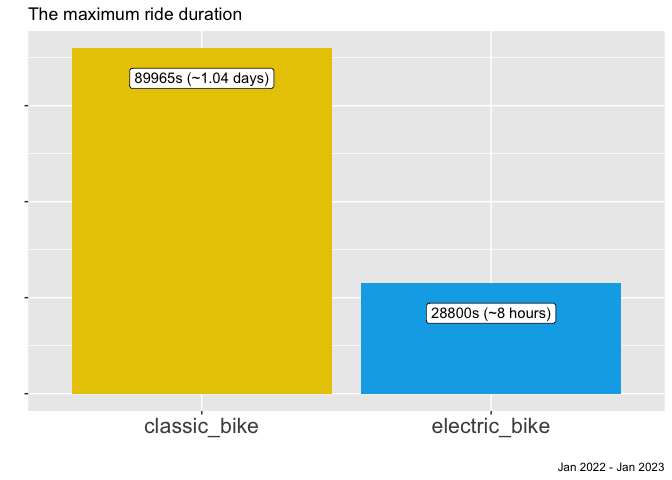
\includegraphics{CS_3_files/figure-latex/maximum ride duration-1.pdf}

\begin{Shaded}
\begin{Highlighting}[]
\NormalTok{raw\_df }\SpecialCharTok{\%\textgreater{}\%} 
  \FunctionTok{filter}\NormalTok{(rideable\_type }\SpecialCharTok{==} \StringTok{"electric\_bike"}\NormalTok{) }\SpecialCharTok{\%\textgreater{}\%}
  \FunctionTok{filter}\NormalTok{(start\_station\_name }\SpecialCharTok{!=}\StringTok{""} \SpecialCharTok{\&}\NormalTok{ end\_station\_name }\SpecialCharTok{!=} \StringTok{""} \SpecialCharTok{\&}
           \SpecialCharTok{!}\FunctionTok{is.na}\NormalTok{(end\_lat)) }\SpecialCharTok{\%\textgreater{}\%} 
  \FunctionTok{select}\NormalTok{(}\StringTok{"rideable\_type"}\NormalTok{, }\StringTok{"member\_casual"}\NormalTok{, }\StringTok{"trip\_duration"}\NormalTok{) }\SpecialCharTok{\%\textgreater{}\%} 
  \FunctionTok{arrange}\NormalTok{(}\FunctionTok{desc}\NormalTok{(trip\_duration)) }\SpecialCharTok{\%\textgreater{}\%} 
  \FunctionTok{head}\NormalTok{(}\DecValTok{30}\NormalTok{)}
\end{Highlighting}
\end{Shaded}

\begin{verbatim}
##    rideable_type member_casual trip_duration
## 1  electric_bike        member      480.0000
## 2  electric_bike        member      479.9833
## 3  electric_bike        casual      479.9167
## 4  electric_bike        member      478.6000
## 5  electric_bike        member      478.5333
## 6  electric_bike        member      477.3000
## 7  electric_bike        member      475.2833
## 8  electric_bike        member      473.2000
## 9  electric_bike        member      471.2667
## 10 electric_bike        member      470.6667
## 11 electric_bike        member      470.2167
## 12 electric_bike        member      468.6500
## 13 electric_bike        member      468.0000
## 14 electric_bike        member      465.8500
## 15 electric_bike        member      465.3000
## 16 electric_bike        member      464.6500
## 17 electric_bike        member      463.9333
## 18 electric_bike        casual      454.6167
## 19 electric_bike        member      449.3333
## 20 electric_bike        member      448.3500
## 21 electric_bike        member      442.0167
## 22 electric_bike        member      441.9667
## 23 electric_bike        member      440.7667
## 24 electric_bike        member      438.8000
## 25 electric_bike        member      430.8000
## 26 electric_bike        member      429.5000
## 27 electric_bike        member      427.7667
## 28 electric_bike        member      425.0500
## 29 electric_bike        member      423.5667
## 30 electric_bike        member      422.6833
\end{verbatim}

Insights:

\begin{itemize}
\item
  Classic bike still leads the way in 1 full day trips
\item
  The electric bike was able to last for 8 hours)
\item
  The absolute majority of long rides on e-bikes were taken by members.
  (Pricing starts at \$1 to unlock plus \$0.39/minute for casual riders
  (\$0 to unlock plus \textbf{\$0.16/minute for members)}.)
\end{itemize}

\hypertarget{number-of-trips-throughout-a-year}{%
\paragraph{Number of trips throughout a
year}\label{number-of-trips-throughout-a-year}}

\begin{Shaded}
\begin{Highlighting}[]
\NormalTok{df }\SpecialCharTok{\%\textgreater{}\%} 
  \FunctionTok{filter}\NormalTok{(started\_at }\SpecialCharTok{\textless{}} \FunctionTok{ymd}\NormalTok{(}\StringTok{"2023{-}01{-}01"}\NormalTok{)) }\SpecialCharTok{\%\textgreater{}\%} \CommentTok{\# limit to a calendar year  }
  \FunctionTok{group\_by}\NormalTok{(member\_casual, rideable\_type) }\SpecialCharTok{\%\textgreater{}\%} 
  \FunctionTok{summarise}\NormalTok{(}\AttributeTok{ride\_count =} \FunctionTok{n}\NormalTok{()) }\SpecialCharTok{\%\textgreater{}\%}
  
  \FunctionTok{ggplot}\NormalTok{() }\SpecialCharTok{+} 
  \FunctionTok{geom\_col}\NormalTok{(}\FunctionTok{aes}\NormalTok{(}\AttributeTok{x =}\NormalTok{ member\_casual, }\AttributeTok{y =}\NormalTok{ ride\_count,  }\AttributeTok{fill =}\NormalTok{ rideable\_type ),}
           \AttributeTok{show.legend =} \ConstantTok{TRUE}\NormalTok{) }\SpecialCharTok{+} 
  \FunctionTok{geom\_label}\NormalTok{(}\FunctionTok{aes}\NormalTok{(}\AttributeTok{x =}\NormalTok{ member\_casual, }\AttributeTok{y =}\NormalTok{ ride\_count,  }
                 \AttributeTok{label =} \FunctionTok{format}\NormalTok{(ride\_count,}\AttributeTok{big.mark=}\StringTok{","}\NormalTok{) , }\AttributeTok{color =}\NormalTok{ rideable\_type),}
             \AttributeTok{position =} \FunctionTok{position\_stack}\NormalTok{(}\AttributeTok{vjust =} \FloatTok{0.6}\NormalTok{) , }\AttributeTok{show.legend =} \ConstantTok{FALSE}\NormalTok{) }\SpecialCharTok{+} 
  \FunctionTok{labs}\NormalTok{(}\AttributeTok{title =} \StringTok{"Number of trips per year"}\NormalTok{, }
       \AttributeTok{caption =} \StringTok{"2022 calendar year data"}\NormalTok{,}
       \AttributeTok{x =}\StringTok{""}\NormalTok{, }\AttributeTok{y=} \StringTok{""}\NormalTok{) }\SpecialCharTok{+}  
  \FunctionTok{scale\_y\_continuous}\NormalTok{(}\AttributeTok{labels =} \FunctionTok{label\_comma}\NormalTok{()) }\SpecialCharTok{+}
  \FunctionTok{theme}\NormalTok{(}\AttributeTok{axis.text =} \FunctionTok{element\_text}\NormalTok{(}\AttributeTok{size =} \DecValTok{16}\NormalTok{) ) }
\end{Highlighting}
\end{Shaded}

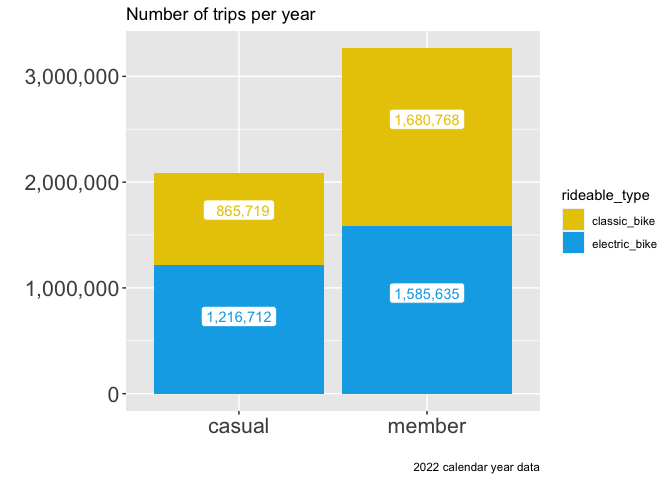
\includegraphics{CS_3_files/figure-latex/Number of trips throughout a year-1.pdf}

\begin{Shaded}
\begin{Highlighting}[]
\NormalTok{df }\SpecialCharTok{\%\textgreater{}\%} 
  \FunctionTok{filter}\NormalTok{(started\_at }\SpecialCharTok{\textless{}} \FunctionTok{ymd}\NormalTok{(}\StringTok{"2023{-}01{-}01"}\NormalTok{)) }\SpecialCharTok{\%\textgreater{}\%} \CommentTok{\# limit to a calendar year }
  \FunctionTok{crosstable}\NormalTok{(}\FunctionTok{c}\NormalTok{(}\StringTok{" "}\OtherTok{=}\NormalTok{rideable\_type), }\AttributeTok{by=}\NormalTok{member\_casual, }\AttributeTok{total=}\StringTok{"both"}\NormalTok{, }\AttributeTok{showNA=}\StringTok{"no"}\NormalTok{, }
        \AttributeTok{percent\_digits=}\DecValTok{0}\NormalTok{, }\AttributeTok{percent\_pattern=}\StringTok{"\{n\} (\{p\_col\})"}\NormalTok{) }\SpecialCharTok{\%\textgreater{}\%} 
  \FunctionTok{as\_flextable}\NormalTok{(}\AttributeTok{compact=}\ConstantTok{TRUE}\NormalTok{, }\AttributeTok{keep\_id=}\ConstantTok{FALSE}\NormalTok{) }\SpecialCharTok{\%\textgreater{}\%} 
  \FunctionTok{set\_caption}\NormalTok{(}\FunctionTok{paste}\NormalTok{(}\StringTok{"Number of trips. 2022 calendar year"}\NormalTok{))}
\end{Highlighting}
\end{Shaded}

\global\setlength{\Oldarrayrulewidth}{\arrayrulewidth}

\global\setlength{\Oldtabcolsep}{\tabcolsep}

\setlength{\tabcolsep}{0pt}

\renewcommand*{\arraystretch}{1.5}



\providecommand{\ascline}[3]{\noalign{\global\arrayrulewidth #1}\arrayrulecolor[HTML]{#2}\cline{#3}}

\begin{longtable}[c]{|p{1.50in}|p{1.33in}|p{1.33in}|p{1.41in}}

\caption{Number\ of\ trips.\ 2022\ calendar\ year}\\

\ascline{1.5pt}{000000}{1-4}

\multicolumn{1}{>{\centering}m{\dimexpr 1.5in+0\tabcolsep}}{} & \multicolumn{2}{>{\centering}m{\dimexpr 2.66in+2\tabcolsep}}{\textcolor[HTML]{000000}{\fontsize{11}{11}\selectfont{\textbf{member\_casual}}}} & \multicolumn{1}{>{\centering}m{\dimexpr 1.41in+0\tabcolsep}}{} \\

\ascline{1pt}{000000}{2-3}



\multicolumn{1}{>{\centering}m{\dimexpr 1.5in+0\tabcolsep}}{\multirow[c]{-2}{*}{\parbox{1.5in}{\textcolor[HTML]{000000}{\fontsize{11}{11}\selectfont{\textbf{}}}}}} & \multicolumn{1}{>{\centering}m{\dimexpr 1.33in+0\tabcolsep}}{\textcolor[HTML]{000000}{\fontsize{11}{11}\selectfont{\textbf{casual}}}} & \multicolumn{1}{>{\centering}m{\dimexpr 1.33in+0\tabcolsep}}{\textcolor[HTML]{000000}{\fontsize{11}{11}\selectfont{\textbf{member}}}} & \multicolumn{1}{>{\centering}m{\dimexpr 1.41in+0\tabcolsep}}{\multirow[c]{-2}{*}{\parbox{1.41in}{\textcolor[HTML]{000000}{\fontsize{11}{11}\selectfont{\textbf{Total}}}}}} \\

\ascline{1.5pt}{000000}{1-4}\endhead



\multicolumn{1}{>{\raggedright}m{\dimexpr 1.5in+0\tabcolsep}}{\textcolor[HTML]{000000}{\fontsize{11}{11}\selectfont{\textbf{\ }}}} & \multicolumn{1}{>{\raggedright}m{\dimexpr 1.33in+0\tabcolsep}}{\textcolor[HTML]{000000}{\fontsize{11}{11}\selectfont{\textbf{}}}} & \multicolumn{1}{>{\raggedright}m{\dimexpr 1.33in+0\tabcolsep}}{\textcolor[HTML]{000000}{\fontsize{11}{11}\selectfont{}}} & \multicolumn{1}{>{\raggedright}m{\dimexpr 1.41in+0\tabcolsep}}{\textcolor[HTML]{000000}{\fontsize{11}{11}\selectfont{}}} \\





\multicolumn{1}{>{\raggedright}m{\dimexpr 1.5in+0\tabcolsep}}{\textcolor[HTML]{000000}{\fontsize{11}{11}\selectfont{classic\_bike}}} & \multicolumn{1}{>{\raggedright}m{\dimexpr 1.33in+0\tabcolsep}}{\textcolor[HTML]{000000}{\fontsize{11}{11}\selectfont{865719\ (42\%)}}} & \multicolumn{1}{>{\raggedright}m{\dimexpr 1.33in+0\tabcolsep}}{\textcolor[HTML]{000000}{\fontsize{11}{11}\selectfont{1680768\ (51\%)}}} & \multicolumn{1}{>{\raggedright}m{\dimexpr 1.41in+0\tabcolsep}}{\textcolor[HTML]{000000}{\fontsize{11}{11}\selectfont{2546487\ (48\%)}}} \\





\multicolumn{1}{>{\raggedright}m{\dimexpr 1.5in+0\tabcolsep}}{\textcolor[HTML]{000000}{\fontsize{11}{11}\selectfont{electric\_bike}}} & \multicolumn{1}{>{\raggedright}m{\dimexpr 1.33in+0\tabcolsep}}{\textcolor[HTML]{000000}{\fontsize{11}{11}\selectfont{1216712\ (58\%)}}} & \multicolumn{1}{>{\raggedright}m{\dimexpr 1.33in+0\tabcolsep}}{\textcolor[HTML]{000000}{\fontsize{11}{11}\selectfont{1585635\ (49\%)}}} & \multicolumn{1}{>{\raggedright}m{\dimexpr 1.41in+0\tabcolsep}}{\textcolor[HTML]{000000}{\fontsize{11}{11}\selectfont{2802347\ (52\%)}}} \\





\multicolumn{1}{>{\raggedright}m{\dimexpr 1.5in+0\tabcolsep}}{\textcolor[HTML]{000000}{\fontsize{11}{11}\selectfont{Total}}} & \multicolumn{1}{>{\raggedright}m{\dimexpr 1.33in+0\tabcolsep}}{\textcolor[HTML]{000000}{\fontsize{11}{11}\selectfont{2082431\ (39\%)}}} & \multicolumn{1}{>{\raggedright}m{\dimexpr 1.33in+0\tabcolsep}}{\textcolor[HTML]{000000}{\fontsize{11}{11}\selectfont{3266403\ (61\%)}}} & \multicolumn{1}{>{\raggedright}m{\dimexpr 1.41in+0\tabcolsep}}{\textcolor[HTML]{000000}{\fontsize{11}{11}\selectfont{5348834\ (100\%)}}} \\

\ascline{1.5pt}{666666}{1-4}



\end{longtable}



\arrayrulecolor[HTML]{000000}

\global\setlength{\arrayrulewidth}{\Oldarrayrulewidth}

\global\setlength{\tabcolsep}{\Oldtabcolsep}

\renewcommand*{\arraystretch}{1}

\begin{Shaded}
\begin{Highlighting}[]
\NormalTok{df }\SpecialCharTok{\%\textgreater{}\%} 
  \FunctionTok{filter}\NormalTok{(started\_at }\SpecialCharTok{\textless{}} \FunctionTok{ymd}\NormalTok{(}\StringTok{"2023{-}01{-}01"}\NormalTok{)) }\SpecialCharTok{\%\textgreater{}\%} \CommentTok{\# limit to a calendar year }
  \FunctionTok{mutate}\NormalTok{(}\AttributeTok{Month=}  \FunctionTok{month}\NormalTok{(started\_at, }\AttributeTok{label =} \ConstantTok{TRUE}\NormalTok{)) }\SpecialCharTok{\%\textgreater{}\%} 
  \FunctionTok{crosstable}\NormalTok{(}\FunctionTok{c}\NormalTok{(}\StringTok{" "}\OtherTok{=}\NormalTok{ Month), }\AttributeTok{by=}\NormalTok{member\_casual, }\AttributeTok{total=}\StringTok{"both"}\NormalTok{, }\AttributeTok{showNA=}\StringTok{"no"}\NormalTok{, }
        \AttributeTok{percent\_digits=}\DecValTok{0}\NormalTok{, }\AttributeTok{percent\_pattern=}\StringTok{"\{n\} (\{p\_col\})"}\NormalTok{) }\SpecialCharTok{\%\textgreater{}\%} 
  \FunctionTok{as\_flextable}\NormalTok{(}\AttributeTok{compact=}\ConstantTok{TRUE}\NormalTok{, }\AttributeTok{keep\_id=}\ConstantTok{FALSE}\NormalTok{) }\SpecialCharTok{\%\textgreater{}\%} 
  \FunctionTok{set\_caption}\NormalTok{(}\FunctionTok{paste}\NormalTok{(}\StringTok{"Number of trips. 2022 calendar year"}\NormalTok{))}
\end{Highlighting}
\end{Shaded}

\global\setlength{\Oldarrayrulewidth}{\arrayrulewidth}

\global\setlength{\Oldtabcolsep}{\tabcolsep}

\setlength{\tabcolsep}{0pt}

\renewcommand*{\arraystretch}{1.5}



\providecommand{\ascline}[3]{\noalign{\global\arrayrulewidth #1}\arrayrulecolor[HTML]{#2}\cline{#3}}

\begin{longtable}[c]{|p{1.00in}|p{1.33in}|p{1.33in}|p{1.41in}}

\caption{Number\ of\ trips.\ 2022\ calendar\ year}\\

\ascline{1.5pt}{000000}{1-4}

\multicolumn{1}{>{\centering}m{\dimexpr 1in+0\tabcolsep}}{} & \multicolumn{2}{>{\centering}m{\dimexpr 2.66in+2\tabcolsep}}{\textcolor[HTML]{000000}{\fontsize{11}{11}\selectfont{\textbf{member\_casual}}}} & \multicolumn{1}{>{\centering}m{\dimexpr 1.41in+0\tabcolsep}}{} \\

\ascline{1pt}{000000}{2-3}



\multicolumn{1}{>{\centering}m{\dimexpr 1in+0\tabcolsep}}{\multirow[c]{-2}{*}{\parbox{1in}{\textcolor[HTML]{000000}{\fontsize{11}{11}\selectfont{\textbf{}}}}}} & \multicolumn{1}{>{\centering}m{\dimexpr 1.33in+0\tabcolsep}}{\textcolor[HTML]{000000}{\fontsize{11}{11}\selectfont{\textbf{casual}}}} & \multicolumn{1}{>{\centering}m{\dimexpr 1.33in+0\tabcolsep}}{\textcolor[HTML]{000000}{\fontsize{11}{11}\selectfont{\textbf{member}}}} & \multicolumn{1}{>{\centering}m{\dimexpr 1.41in+0\tabcolsep}}{\multirow[c]{-2}{*}{\parbox{1.41in}{\textcolor[HTML]{000000}{\fontsize{11}{11}\selectfont{\textbf{Total}}}}}} \\

\ascline{1.5pt}{000000}{1-4}\endhead



\multicolumn{1}{>{\raggedright}m{\dimexpr 1in+0\tabcolsep}}{\textcolor[HTML]{000000}{\fontsize{11}{11}\selectfont{\textbf{\ }}}} & \multicolumn{1}{>{\raggedright}m{\dimexpr 1.33in+0\tabcolsep}}{\textcolor[HTML]{000000}{\fontsize{11}{11}\selectfont{\textbf{}}}} & \multicolumn{1}{>{\raggedright}m{\dimexpr 1.33in+0\tabcolsep}}{\textcolor[HTML]{000000}{\fontsize{11}{11}\selectfont{}}} & \multicolumn{1}{>{\raggedright}m{\dimexpr 1.41in+0\tabcolsep}}{\textcolor[HTML]{000000}{\fontsize{11}{11}\selectfont{}}} \\





\multicolumn{1}{>{\raggedright}m{\dimexpr 1in+0\tabcolsep}}{\textcolor[HTML]{000000}{\fontsize{11}{11}\selectfont{Jan}}} & \multicolumn{1}{>{\raggedright}m{\dimexpr 1.33in+0\tabcolsep}}{\textcolor[HTML]{000000}{\fontsize{11}{11}\selectfont{16997\ (1\%)}}} & \multicolumn{1}{>{\raggedright}m{\dimexpr 1.33in+0\tabcolsep}}{\textcolor[HTML]{000000}{\fontsize{11}{11}\selectfont{83482\ (3\%)}}} & \multicolumn{1}{>{\raggedright}m{\dimexpr 1.41in+0\tabcolsep}}{\textcolor[HTML]{000000}{\fontsize{11}{11}\selectfont{100479\ (2\%)}}} \\





\multicolumn{1}{>{\raggedright}m{\dimexpr 1in+0\tabcolsep}}{\textcolor[HTML]{000000}{\fontsize{11}{11}\selectfont{Feb}}} & \multicolumn{1}{>{\raggedright}m{\dimexpr 1.33in+0\tabcolsep}}{\textcolor[HTML]{000000}{\fontsize{11}{11}\selectfont{19376\ (1\%)}}} & \multicolumn{1}{>{\raggedright}m{\dimexpr 1.33in+0\tabcolsep}}{\textcolor[HTML]{000000}{\fontsize{11}{11}\selectfont{91871\ (3\%)}}} & \multicolumn{1}{>{\raggedright}m{\dimexpr 1.41in+0\tabcolsep}}{\textcolor[HTML]{000000}{\fontsize{11}{11}\selectfont{111247\ (2\%)}}} \\





\multicolumn{1}{>{\raggedright}m{\dimexpr 1in+0\tabcolsep}}{\textcolor[HTML]{000000}{\fontsize{11}{11}\selectfont{Mar}}} & \multicolumn{1}{>{\raggedright}m{\dimexpr 1.33in+0\tabcolsep}}{\textcolor[HTML]{000000}{\fontsize{11}{11}\selectfont{79311\ (4\%)}}} & \multicolumn{1}{>{\raggedright}m{\dimexpr 1.33in+0\tabcolsep}}{\textcolor[HTML]{000000}{\fontsize{11}{11}\selectfont{190241\ (6\%)}}} & \multicolumn{1}{>{\raggedright}m{\dimexpr 1.41in+0\tabcolsep}}{\textcolor[HTML]{000000}{\fontsize{11}{11}\selectfont{269552\ (5\%)}}} \\





\multicolumn{1}{>{\raggedright}m{\dimexpr 1in+0\tabcolsep}}{\textcolor[HTML]{000000}{\fontsize{11}{11}\selectfont{Apr}}} & \multicolumn{1}{>{\raggedright}m{\dimexpr 1.33in+0\tabcolsep}}{\textcolor[HTML]{000000}{\fontsize{11}{11}\selectfont{111128\ (5\%)}}} & \multicolumn{1}{>{\raggedright}m{\dimexpr 1.33in+0\tabcolsep}}{\textcolor[HTML]{000000}{\fontsize{11}{11}\selectfont{239523\ (7\%)}}} & \multicolumn{1}{>{\raggedright}m{\dimexpr 1.41in+0\tabcolsep}}{\textcolor[HTML]{000000}{\fontsize{11}{11}\selectfont{350651\ (7\%)}}} \\





\multicolumn{1}{>{\raggedright}m{\dimexpr 1in+0\tabcolsep}}{\textcolor[HTML]{000000}{\fontsize{11}{11}\selectfont{May}}} & \multicolumn{1}{>{\raggedright}m{\dimexpr 1.33in+0\tabcolsep}}{\textcolor[HTML]{000000}{\fontsize{11}{11}\selectfont{246537\ (12\%)}}} & \multicolumn{1}{>{\raggedright}m{\dimexpr 1.33in+0\tabcolsep}}{\textcolor[HTML]{000000}{\fontsize{11}{11}\selectfont{346854\ (11\%)}}} & \multicolumn{1}{>{\raggedright}m{\dimexpr 1.41in+0\tabcolsep}}{\textcolor[HTML]{000000}{\fontsize{11}{11}\selectfont{593391\ (11\%)}}} \\





\multicolumn{1}{>{\raggedright}m{\dimexpr 1in+0\tabcolsep}}{\textcolor[HTML]{000000}{\fontsize{11}{11}\selectfont{Jun}}} & \multicolumn{1}{>{\raggedright}m{\dimexpr 1.33in+0\tabcolsep}}{\textcolor[HTML]{000000}{\fontsize{11}{11}\selectfont{328588\ (16\%)}}} & \multicolumn{1}{>{\raggedright}m{\dimexpr 1.33in+0\tabcolsep}}{\textcolor[HTML]{000000}{\fontsize{11}{11}\selectfont{391205\ (12\%)}}} & \multicolumn{1}{>{\raggedright}m{\dimexpr 1.41in+0\tabcolsep}}{\textcolor[HTML]{000000}{\fontsize{11}{11}\selectfont{719793\ (13\%)}}} \\





\multicolumn{1}{>{\raggedright}m{\dimexpr 1in+0\tabcolsep}}{\textcolor[HTML]{000000}{\fontsize{11}{11}\selectfont{Jul}}} & \multicolumn{1}{>{\raggedright}m{\dimexpr 1.33in+0\tabcolsep}}{\textcolor[HTML]{000000}{\fontsize{11}{11}\selectfont{363992\ (17\%)}}} & \multicolumn{1}{>{\raggedright}m{\dimexpr 1.33in+0\tabcolsep}}{\textcolor[HTML]{000000}{\fontsize{11}{11}\selectfont{407415\ (12\%)}}} & \multicolumn{1}{>{\raggedright}m{\dimexpr 1.41in+0\tabcolsep}}{\textcolor[HTML]{000000}{\fontsize{11}{11}\selectfont{771407\ (14\%)}}} \\





\multicolumn{1}{>{\raggedright}m{\dimexpr 1in+0\tabcolsep}}{\textcolor[HTML]{000000}{\fontsize{11}{11}\selectfont{Aug}}} & \multicolumn{1}{>{\raggedright}m{\dimexpr 1.33in+0\tabcolsep}}{\textcolor[HTML]{000000}{\fontsize{11}{11}\selectfont{322906\ (16\%)}}} & \multicolumn{1}{>{\raggedright}m{\dimexpr 1.33in+0\tabcolsep}}{\textcolor[HTML]{000000}{\fontsize{11}{11}\selectfont{416457\ (13\%)}}} & \multicolumn{1}{>{\raggedright}m{\dimexpr 1.41in+0\tabcolsep}}{\textcolor[HTML]{000000}{\fontsize{11}{11}\selectfont{739363\ (14\%)}}} \\





\multicolumn{1}{>{\raggedright}m{\dimexpr 1in+0\tabcolsep}}{\textcolor[HTML]{000000}{\fontsize{11}{11}\selectfont{Sep}}} & \multicolumn{1}{>{\raggedright}m{\dimexpr 1.33in+0\tabcolsep}}{\textcolor[HTML]{000000}{\fontsize{11}{11}\selectfont{269081\ (13\%)}}} & \multicolumn{1}{>{\raggedright}m{\dimexpr 1.33in+0\tabcolsep}}{\textcolor[HTML]{000000}{\fontsize{11}{11}\selectfont{394612\ (12\%)}}} & \multicolumn{1}{>{\raggedright}m{\dimexpr 1.41in+0\tabcolsep}}{\textcolor[HTML]{000000}{\fontsize{11}{11}\selectfont{663693\ (12\%)}}} \\





\multicolumn{1}{>{\raggedright}m{\dimexpr 1in+0\tabcolsep}}{\textcolor[HTML]{000000}{\fontsize{11}{11}\selectfont{Oct}}} & \multicolumn{1}{>{\raggedright}m{\dimexpr 1.33in+0\tabcolsep}}{\textcolor[HTML]{000000}{\fontsize{11}{11}\selectfont{190741\ (9\%)}}} & \multicolumn{1}{>{\raggedright}m{\dimexpr 1.33in+0\tabcolsep}}{\textcolor[HTML]{000000}{\fontsize{11}{11}\selectfont{340655\ (10\%)}}} & \multicolumn{1}{>{\raggedright}m{\dimexpr 1.41in+0\tabcolsep}}{\textcolor[HTML]{000000}{\fontsize{11}{11}\selectfont{531396\ (10\%)}}} \\





\multicolumn{1}{>{\raggedright}m{\dimexpr 1in+0\tabcolsep}}{\textcolor[HTML]{000000}{\fontsize{11}{11}\selectfont{Nov}}} & \multicolumn{1}{>{\raggedright}m{\dimexpr 1.33in+0\tabcolsep}}{\textcolor[HTML]{000000}{\fontsize{11}{11}\selectfont{92165\ (4\%)}}} & \multicolumn{1}{>{\raggedright}m{\dimexpr 1.33in+0\tabcolsep}}{\textcolor[HTML]{000000}{\fontsize{11}{11}\selectfont{231179\ (7\%)}}} & \multicolumn{1}{>{\raggedright}m{\dimexpr 1.41in+0\tabcolsep}}{\textcolor[HTML]{000000}{\fontsize{11}{11}\selectfont{323344\ (6\%)}}} \\





\multicolumn{1}{>{\raggedright}m{\dimexpr 1in+0\tabcolsep}}{\textcolor[HTML]{000000}{\fontsize{11}{11}\selectfont{Dec}}} & \multicolumn{1}{>{\raggedright}m{\dimexpr 1.33in+0\tabcolsep}}{\textcolor[HTML]{000000}{\fontsize{11}{11}\selectfont{41609\ (2\%)}}} & \multicolumn{1}{>{\raggedright}m{\dimexpr 1.33in+0\tabcolsep}}{\textcolor[HTML]{000000}{\fontsize{11}{11}\selectfont{132909\ (4\%)}}} & \multicolumn{1}{>{\raggedright}m{\dimexpr 1.41in+0\tabcolsep}}{\textcolor[HTML]{000000}{\fontsize{11}{11}\selectfont{174518\ (3\%)}}} \\





\multicolumn{1}{>{\raggedright}m{\dimexpr 1in+0\tabcolsep}}{\textcolor[HTML]{000000}{\fontsize{11}{11}\selectfont{Total}}} & \multicolumn{1}{>{\raggedright}m{\dimexpr 1.33in+0\tabcolsep}}{\textcolor[HTML]{000000}{\fontsize{11}{11}\selectfont{2082431\ (39\%)}}} & \multicolumn{1}{>{\raggedright}m{\dimexpr 1.33in+0\tabcolsep}}{\textcolor[HTML]{000000}{\fontsize{11}{11}\selectfont{3266403\ (61\%)}}} & \multicolumn{1}{>{\raggedright}m{\dimexpr 1.41in+0\tabcolsep}}{\textcolor[HTML]{000000}{\fontsize{11}{11}\selectfont{5348834\ (100\%)}}} \\

\ascline{1.5pt}{666666}{1-4}



\end{longtable}



\arrayrulecolor[HTML]{000000}

\global\setlength{\arrayrulewidth}{\Oldarrayrulewidth}

\global\setlength{\tabcolsep}{\Oldtabcolsep}

\renewcommand*{\arraystretch}{1}

\begin{longtable}[]{@{}
  >{\raggedright\arraybackslash}p{(\columnwidth - 0\tabcolsep) * \real{1.0110}}@{}}
\toprule()
\begin{minipage}[b]{\linewidth}\raggedright
Number of trips
\end{minipage} \\
\midrule()
\endhead
\begin{minipage}[t]{\linewidth}\raggedright
\begin{itemize}
\tightlist
\item
  \textbf{Casual} riders \textbf{prefer e-bikes}
\end{itemize}
\end{minipage} \\
\begin{minipage}[t]{\linewidth}\raggedright
\begin{itemize}
\tightlist
\item
  while Cyclistic's \textbf{members} choose e-bikes and classic bikes
  roughly equally
\end{itemize}
\end{minipage} \\
\begin{minipage}[t]{\linewidth}\raggedright
\begin{itemize}
\tightlist
\item
  \textbf{Members} use Cyclistics's services \textbf{much more often}
  than casual riders (+50 \%).
\end{itemize}
\end{minipage} \\
\bottomrule()
\end{longtable}

\hypertarget{the-mode-of-day-of-week-throughout-a-year}{%
\paragraph{The mode of day of week throughout a
year}\label{the-mode-of-day-of-week-throughout-a-year}}

\begin{Shaded}
\begin{Highlighting}[]
\NormalTok{Mode }\OtherTok{\textless{}{-}} \ControlFlowTok{function}\NormalTok{(x) \{}
\NormalTok{  ux }\OtherTok{\textless{}{-}} \FunctionTok{unique}\NormalTok{(x)}
\NormalTok{  ux[}\FunctionTok{which.max}\NormalTok{(}\FunctionTok{tabulate}\NormalTok{(}\FunctionTok{match}\NormalTok{(x, ux)))]}
\NormalTok{\}}

\NormalTok{num\_weeks }\OtherTok{\textless{}{-}} \FunctionTok{as.numeric}\NormalTok{(}\FunctionTok{max}\NormalTok{(df}\SpecialCharTok{$}\NormalTok{ended\_at) }\SpecialCharTok{{-}} \FunctionTok{min}\NormalTok{(df}\SpecialCharTok{$}\NormalTok{ended\_at),}\StringTok{"weeks"}\NormalTok{) }
\NormalTok{df }\SpecialCharTok{\%\textgreater{}\%} 
  \FunctionTok{group\_by}\NormalTok{(member\_casual, weekday) }\SpecialCharTok{\%\textgreater{}\%}
  \FunctionTok{summarise}\NormalTok{(}\AttributeTok{mode =} \FunctionTok{Mode}\NormalTok{(weekday), }
            \AttributeTok{count =} \FunctionTok{n}\NormalTok{() }\SpecialCharTok{/}\NormalTok{ num\_weeks )  }\SpecialCharTok{\%\textgreater{}\%} 
  \CommentTok{\# arrange(desc(count))}
  
  \FunctionTok{ggplot}\NormalTok{() }\SpecialCharTok{+}
  \FunctionTok{geom\_col}\NormalTok{(}\FunctionTok{aes}\NormalTok{(}\AttributeTok{y =}\NormalTok{ count, }\AttributeTok{x =}\NormalTok{ weekday, }\AttributeTok{fill =}\NormalTok{ member\_casual ),}
           \AttributeTok{position =} \StringTok{"stack"}\NormalTok{) }\SpecialCharTok{+} \CommentTok{\#, show.legend = FALSE, , alpha = 0.8}
  \FunctionTok{labs}\NormalTok{(}\AttributeTok{title =} \StringTok{"Number of trips by day of the week"}\NormalTok{,}
       \AttributeTok{caption =}\NormalTok{ report\_caption,}
       \AttributeTok{x =}\StringTok{""}\NormalTok{, }\AttributeTok{y=} \StringTok{"Stacked count"}\NormalTok{,}
       \AttributeTok{fill=}\StringTok{\textquotesingle{}Type of rider\textquotesingle{}}\NormalTok{) }\SpecialCharTok{+}
  \FunctionTok{scale\_y\_continuous}\NormalTok{(}\AttributeTok{labels =} \FunctionTok{label\_comma}\NormalTok{()) }\SpecialCharTok{+}
  \FunctionTok{geom\_label}\NormalTok{(}\FunctionTok{aes}\NormalTok{(}\AttributeTok{x =}\NormalTok{ weekday, }\AttributeTok{y =}\NormalTok{ count,  }\AttributeTok{label =} \FunctionTok{round}\NormalTok{(count), }\AttributeTok{color =}\NormalTok{ member\_casual), }
      \AttributeTok{hjust =}\FloatTok{0.5}\NormalTok{, }\AttributeTok{vjust =} \FloatTok{1.7}\NormalTok{, }\AttributeTok{show.legend =} \ConstantTok{FALSE}\NormalTok{, }\AttributeTok{size =} \DecValTok{3}\NormalTok{,}
      \AttributeTok{position =} \StringTok{"stack"}\NormalTok{) }\CommentTok{\# position\_dodge(width = 1)}
\end{Highlighting}
\end{Shaded}

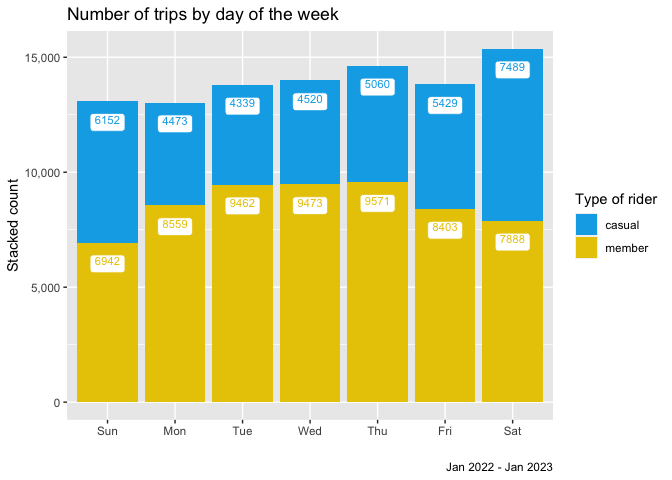
\includegraphics{CS_3_files/figure-latex/overall mode of day of week-1.pdf}

\begin{Shaded}
\begin{Highlighting}[]
\NormalTok{Mode }\OtherTok{\textless{}{-}} \ControlFlowTok{function}\NormalTok{(x) \{}
\NormalTok{  ux }\OtherTok{\textless{}{-}} \FunctionTok{unique}\NormalTok{(x)}
\NormalTok{  ux[}\FunctionTok{which.max}\NormalTok{(}\FunctionTok{tabulate}\NormalTok{(}\FunctionTok{match}\NormalTok{(x, ux)))]}
\NormalTok{\}}

\NormalTok{num\_weeks }\OtherTok{\textless{}{-}} \FunctionTok{as.numeric}\NormalTok{(}\FunctionTok{max}\NormalTok{(df}\SpecialCharTok{$}\NormalTok{ended\_at) }\SpecialCharTok{{-}} \FunctionTok{min}\NormalTok{(df}\SpecialCharTok{$}\NormalTok{ended\_at),}\StringTok{"weeks"}\NormalTok{) }
\NormalTok{df }\SpecialCharTok{\%\textgreater{}\%} 
  \FunctionTok{group\_by}\NormalTok{(member\_casual, weekday) }\SpecialCharTok{\%\textgreater{}\%}
  \FunctionTok{summarise}\NormalTok{(}\AttributeTok{mode =} \FunctionTok{Mode}\NormalTok{(weekday), }
            \AttributeTok{count =} \FunctionTok{n}\NormalTok{() }\SpecialCharTok{/}\NormalTok{ num\_weeks )  }\SpecialCharTok{\%\textgreater{}\%} 
  \CommentTok{\# arrange(desc(count))}
  
  \FunctionTok{ggplot}\NormalTok{() }\SpecialCharTok{+}
  \FunctionTok{geom\_col}\NormalTok{(}\FunctionTok{aes}\NormalTok{(}\AttributeTok{y =}\NormalTok{ count, }\AttributeTok{x =}\NormalTok{ weekday, }\AttributeTok{fill =}\NormalTok{ member\_casual ),}
           \AttributeTok{position =} \StringTok{"dodge"}\NormalTok{) }\SpecialCharTok{+} \CommentTok{\#, show.legend = FALSE, , alpha = 0.8}
  \FunctionTok{labs}\NormalTok{(}\AttributeTok{title =} \StringTok{"Number of trips by day of the week"}\NormalTok{,}
       \AttributeTok{caption =}\NormalTok{ report\_caption,}
       \AttributeTok{x =}\StringTok{""}\NormalTok{, }\AttributeTok{y=} \StringTok{"Number of trips"}\NormalTok{,}
       \AttributeTok{fill=}\StringTok{\textquotesingle{}Type of rider\textquotesingle{}}\NormalTok{) }\SpecialCharTok{+}
  \FunctionTok{scale\_y\_continuous}\NormalTok{(}\AttributeTok{labels =} \FunctionTok{label\_comma}\NormalTok{()) }\SpecialCharTok{+}
  \FunctionTok{geom\_label}\NormalTok{(}\FunctionTok{aes}\NormalTok{(}\AttributeTok{x =}\NormalTok{ weekday, }\AttributeTok{y =}\NormalTok{ count,  }\AttributeTok{label =} \FunctionTok{round}\NormalTok{(count), }\AttributeTok{color =}\NormalTok{ member\_casual), }
      \AttributeTok{hjust =}\FloatTok{0.5}\NormalTok{, }\AttributeTok{vjust =} \FloatTok{1.7}\NormalTok{, }\AttributeTok{show.legend =} \ConstantTok{FALSE}\NormalTok{, }\AttributeTok{size =} \DecValTok{3}\NormalTok{,}
      \AttributeTok{position =} \FunctionTok{position\_dodge}\NormalTok{(}\AttributeTok{width =} \DecValTok{1}\NormalTok{)) }
\end{Highlighting}
\end{Shaded}

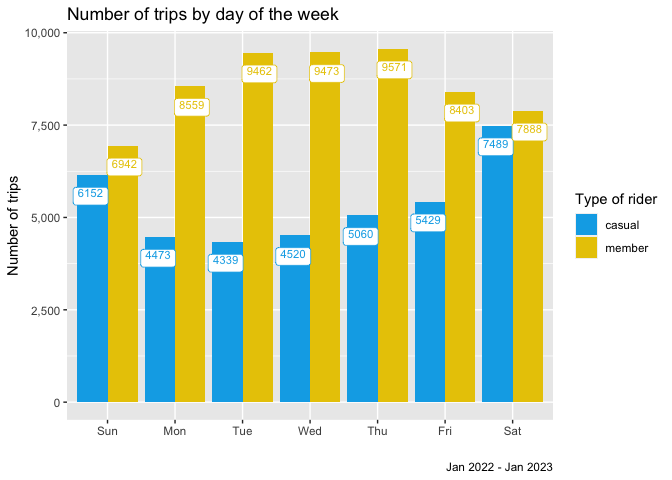
\includegraphics{CS_3_files/figure-latex/mode of dow by member_casual-1.pdf}

\begin{Shaded}
\begin{Highlighting}[]
\NormalTok{Mode }\OtherTok{\textless{}{-}} \ControlFlowTok{function}\NormalTok{(x) \{}
\NormalTok{  ux }\OtherTok{\textless{}{-}} \FunctionTok{unique}\NormalTok{(x)}
\NormalTok{  ux[}\FunctionTok{which.max}\NormalTok{(}\FunctionTok{tabulate}\NormalTok{(}\FunctionTok{match}\NormalTok{(x, ux)))]}
\NormalTok{\}}

\NormalTok{num\_weeks }\OtherTok{\textless{}{-}} \FunctionTok{as.numeric}\NormalTok{(}\FunctionTok{max}\NormalTok{(df}\SpecialCharTok{$}\NormalTok{ended\_at) }\SpecialCharTok{{-}} \FunctionTok{min}\NormalTok{(df}\SpecialCharTok{$}\NormalTok{ended\_at),}\StringTok{"weeks"}\NormalTok{)}

\NormalTok{df }\SpecialCharTok{\%\textgreater{}\%} 
  \FunctionTok{mutate}\NormalTok{(}\AttributeTok{Month=}  \FunctionTok{month}\NormalTok{(started\_at, }\AttributeTok{label =} \ConstantTok{TRUE}\NormalTok{)) }\SpecialCharTok{\%\textgreater{}\%} 

  \FunctionTok{crosstable}\NormalTok{(}\FunctionTok{c}\NormalTok{(}\StringTok{"   "} \OtherTok{=}\NormalTok{Month), }\AttributeTok{by=}\FunctionTok{c}\NormalTok{(}\StringTok{" "}\OtherTok{=}\NormalTok{member\_casual,}\StringTok{"  "}\OtherTok{=}\NormalTok{weekday),  }\AttributeTok{total=}\StringTok{"both"}\NormalTok{, }\AttributeTok{showNA=}\StringTok{"no"}\NormalTok{, }
        \AttributeTok{percent\_digits=}\DecValTok{0}\NormalTok{, }\AttributeTok{percent\_pattern=}\StringTok{"\{n\} (\{p\_col\})"}\NormalTok{) }\SpecialCharTok{\%\textgreater{}\%} 
  \FunctionTok{as\_flextable}\NormalTok{(}\AttributeTok{compact=}\ConstantTok{TRUE}\NormalTok{, }\AttributeTok{keep\_id=}\ConstantTok{FALSE}\NormalTok{) }\SpecialCharTok{\%\textgreater{}\%} 
  \FunctionTok{set\_caption}\NormalTok{(}\FunctionTok{paste}\NormalTok{(}\StringTok{"Cross table. Number of trips by Month and by day of the week"}\NormalTok{, report\_caption))}
\end{Highlighting}
\end{Shaded}

\begin{verbatim}
## Warning: fonts used in `flextable` are ignored because the `pdflatex` engine is
## used and not `xelatex` or `lualatex`. You can avoid this warning by using the
## `set_flextable_defaults(fonts_ignore=TRUE)` command or use a compatible engine
## by defining `latex_engine: xelatex` in the YAML header of the R Markdown
## document.
\end{verbatim}

\global\setlength{\Oldarrayrulewidth}{\arrayrulewidth}

\global\setlength{\Oldtabcolsep}{\tabcolsep}

\setlength{\tabcolsep}{0pt}

\renewcommand*{\arraystretch}{1.5}



\providecommand{\ascline}[3]{\noalign{\global\arrayrulewidth #1}\arrayrulecolor[HTML]{#2}\cline{#3}}

\begin{longtable}[c]{|p{1.00in}|p{1.16in}|p{1.16in}|p{1.16in}|p{1.16in}|p{1.16in}|p{1.24in}|p{1.16in}|p{1.24in}|p{1.16in}|p{1.24in}|p{1.16in}|p{1.16in}|p{1.16in}|p{1.16in}|p{1.41in}}

\caption{Cross\ table.\ Number\ of\ trips\ by\ Month\ and\ by\ day\ of\ the\ week\ Jan\ 2022\ -\ Jan\ 2023}\\

\ascline{1.5pt}{000000}{1-16}

\multicolumn{1}{!{\color[HTML]{000000}\vrule width 1pt}>{\centering}m{\dimexpr 1in+0\tabcolsep}}{} & \multicolumn{2}{!{\color[HTML]{000000}\vrule width 1pt}>{\centering}m{\dimexpr 2.32in+2\tabcolsep}}{\textcolor[HTML]{000000}{\fontsize{11}{11}\selectfont{\textbf{\ \ =Sun}}}} & \multicolumn{2}{!{\color[HTML]{000000}\vrule width 1pt}>{\centering}m{\dimexpr 2.32in+2\tabcolsep}}{\textcolor[HTML]{000000}{\fontsize{11}{11}\selectfont{\textbf{\ \ =Mon}}}} & \multicolumn{2}{!{\color[HTML]{000000}\vrule width 1pt}>{\centering}m{\dimexpr 2.4in+2\tabcolsep}}{\textcolor[HTML]{000000}{\fontsize{11}{11}\selectfont{\textbf{\ \ =Tue}}}} & \multicolumn{2}{!{\color[HTML]{000000}\vrule width 1pt}>{\centering}m{\dimexpr 2.4in+2\tabcolsep}}{\textcolor[HTML]{000000}{\fontsize{11}{11}\selectfont{\textbf{\ \ =Wed}}}} & \multicolumn{2}{!{\color[HTML]{000000}\vrule width 1pt}>{\centering}m{\dimexpr 2.4in+2\tabcolsep}}{\textcolor[HTML]{000000}{\fontsize{11}{11}\selectfont{\textbf{\ \ =Thu}}}} & \multicolumn{2}{!{\color[HTML]{000000}\vrule width 1pt}>{\centering}m{\dimexpr 2.32in+2\tabcolsep}}{\textcolor[HTML]{000000}{\fontsize{11}{11}\selectfont{\textbf{\ \ =Fri}}}} & \multicolumn{2}{!{\color[HTML]{000000}\vrule width 1pt}>{\centering}m{\dimexpr 2.32in+2\tabcolsep}}{\textcolor[HTML]{000000}{\fontsize{11}{11}\selectfont{\textbf{\ \ =Sat}}}} & \multicolumn{1}{!{\color[HTML]{000000}\vrule width 1pt}>{\centering}m{\dimexpr 1.41in+0\tabcolsep}!{\color[HTML]{000000}\vrule width 1pt}}{} \\

\ascline{1pt}{000000}{2-15}



\multicolumn{1}{!{\color[HTML]{000000}\vrule width 1pt}>{\centering}m{\dimexpr 1in+0\tabcolsep}}{\multirow[c]{-2}{*}{\parbox{1in}{\textcolor[HTML]{000000}{\fontsize{11}{11}\selectfont{\textbf{variable}}}}}} & \multicolumn{1}{!{\color[HTML]{000000}\vrule width 1pt}>{\centering}m{\dimexpr 1.16in+0\tabcolsep}}{\textcolor[HTML]{000000}{\fontsize{11}{11}\selectfont{\textbf{\ =casual}}}} & \multicolumn{1}{>{\centering}m{\dimexpr 1.16in+0\tabcolsep}}{\textcolor[HTML]{000000}{\fontsize{11}{11}\selectfont{\textbf{\ =member}}}} & \multicolumn{1}{!{\color[HTML]{000000}\vrule width 1pt}>{\centering}m{\dimexpr 1.16in+0\tabcolsep}}{\textcolor[HTML]{000000}{\fontsize{11}{11}\selectfont{\textbf{\ =casual}}}} & \multicolumn{1}{>{\centering}m{\dimexpr 1.16in+0\tabcolsep}}{\textcolor[HTML]{000000}{\fontsize{11}{11}\selectfont{\textbf{\ =member}}}} & \multicolumn{1}{!{\color[HTML]{000000}\vrule width 1pt}>{\centering}m{\dimexpr 1.16in+0\tabcolsep}}{\textcolor[HTML]{000000}{\fontsize{11}{11}\selectfont{\textbf{\ =casual}}}} & \multicolumn{1}{>{\centering}m{\dimexpr 1.24in+0\tabcolsep}}{\textcolor[HTML]{000000}{\fontsize{11}{11}\selectfont{\textbf{\ =member}}}} & \multicolumn{1}{!{\color[HTML]{000000}\vrule width 1pt}>{\centering}m{\dimexpr 1.16in+0\tabcolsep}}{\textcolor[HTML]{000000}{\fontsize{11}{11}\selectfont{\textbf{\ =casual}}}} & \multicolumn{1}{>{\centering}m{\dimexpr 1.24in+0\tabcolsep}}{\textcolor[HTML]{000000}{\fontsize{11}{11}\selectfont{\textbf{\ =member}}}} & \multicolumn{1}{!{\color[HTML]{000000}\vrule width 1pt}>{\centering}m{\dimexpr 1.16in+0\tabcolsep}}{\textcolor[HTML]{000000}{\fontsize{11}{11}\selectfont{\textbf{\ =casual}}}} & \multicolumn{1}{>{\centering}m{\dimexpr 1.24in+0\tabcolsep}}{\textcolor[HTML]{000000}{\fontsize{11}{11}\selectfont{\textbf{\ =member}}}} & \multicolumn{1}{!{\color[HTML]{000000}\vrule width 1pt}>{\centering}m{\dimexpr 1.16in+0\tabcolsep}}{\textcolor[HTML]{000000}{\fontsize{11}{11}\selectfont{\textbf{\ =casual}}}} & \multicolumn{1}{>{\centering}m{\dimexpr 1.16in+0\tabcolsep}}{\textcolor[HTML]{000000}{\fontsize{11}{11}\selectfont{\textbf{\ =member}}}} & \multicolumn{1}{!{\color[HTML]{000000}\vrule width 1pt}>{\centering}m{\dimexpr 1.16in+0\tabcolsep}}{\textcolor[HTML]{000000}{\fontsize{11}{11}\selectfont{\textbf{\ =casual}}}} & \multicolumn{1}{>{\centering}m{\dimexpr 1.16in+0\tabcolsep}}{\textcolor[HTML]{000000}{\fontsize{11}{11}\selectfont{\textbf{\ =member}}}} & \multicolumn{1}{!{\color[HTML]{000000}\vrule width 1pt}>{\centering}m{\dimexpr 1.41in+0\tabcolsep}!{\color[HTML]{000000}\vrule width 1pt}}{\multirow[c]{-2}{*}{\parbox{1.41in}{\textcolor[HTML]{000000}{\fontsize{11}{11}\selectfont{\textbf{Total}}}}}} \\

\ascline{1.5pt}{000000}{1-16}\endhead



\multicolumn{1}{!{\color[HTML]{000000}\vrule width 1pt}>{\raggedright}m{\dimexpr 1in+0\tabcolsep}}{\textcolor[HTML]{000000}{\fontsize{11}{11}\selectfont{\textbf{\ \ \ }}}} & \multicolumn{1}{!{\color[HTML]{000000}\vrule width 1pt}>{\raggedright}m{\dimexpr 1.16in+0\tabcolsep}}{\textcolor[HTML]{000000}{\fontsize{11}{11}\selectfont{\textbf{}}}} & \multicolumn{1}{>{\raggedright}m{\dimexpr 1.16in+0\tabcolsep}}{\textcolor[HTML]{000000}{\fontsize{11}{11}\selectfont{}}} & \multicolumn{1}{!{\color[HTML]{000000}\vrule width 1pt}>{\raggedright}m{\dimexpr 1.16in+0\tabcolsep}}{\textcolor[HTML]{000000}{\fontsize{11}{11}\selectfont{}}} & \multicolumn{1}{>{\raggedright}m{\dimexpr 1.16in+0\tabcolsep}}{\textcolor[HTML]{000000}{\fontsize{11}{11}\selectfont{}}} & \multicolumn{1}{!{\color[HTML]{000000}\vrule width 1pt}>{\raggedright}m{\dimexpr 1.16in+0\tabcolsep}}{\textcolor[HTML]{000000}{\fontsize{11}{11}\selectfont{}}} & \multicolumn{1}{>{\raggedright}m{\dimexpr 1.24in+0\tabcolsep}}{\textcolor[HTML]{000000}{\fontsize{11}{11}\selectfont{}}} & \multicolumn{1}{!{\color[HTML]{000000}\vrule width 1pt}>{\raggedright}m{\dimexpr 1.16in+0\tabcolsep}}{\textcolor[HTML]{000000}{\fontsize{11}{11}\selectfont{}}} & \multicolumn{1}{>{\raggedright}m{\dimexpr 1.24in+0\tabcolsep}}{\textcolor[HTML]{000000}{\fontsize{11}{11}\selectfont{}}} & \multicolumn{1}{!{\color[HTML]{000000}\vrule width 1pt}>{\raggedright}m{\dimexpr 1.16in+0\tabcolsep}}{\textcolor[HTML]{000000}{\fontsize{11}{11}\selectfont{}}} & \multicolumn{1}{>{\raggedright}m{\dimexpr 1.24in+0\tabcolsep}}{\textcolor[HTML]{000000}{\fontsize{11}{11}\selectfont{}}} & \multicolumn{1}{!{\color[HTML]{000000}\vrule width 1pt}>{\raggedright}m{\dimexpr 1.16in+0\tabcolsep}}{\textcolor[HTML]{000000}{\fontsize{11}{11}\selectfont{}}} & \multicolumn{1}{>{\raggedright}m{\dimexpr 1.16in+0\tabcolsep}}{\textcolor[HTML]{000000}{\fontsize{11}{11}\selectfont{}}} & \multicolumn{1}{!{\color[HTML]{000000}\vrule width 1pt}>{\raggedright}m{\dimexpr 1.16in+0\tabcolsep}}{\textcolor[HTML]{000000}{\fontsize{11}{11}\selectfont{}}} & \multicolumn{1}{>{\raggedright}m{\dimexpr 1.16in+0\tabcolsep}}{\textcolor[HTML]{000000}{\fontsize{11}{11}\selectfont{}}} & \multicolumn{1}{!{\color[HTML]{000000}\vrule width 1pt}>{\raggedright}m{\dimexpr 1.41in+0\tabcolsep}!{\color[HTML]{000000}\vrule width 1pt}}{\textcolor[HTML]{000000}{\fontsize{11}{11}\selectfont{}}} \\





\multicolumn{1}{!{\color[HTML]{000000}\vrule width 1pt}>{\raggedright}m{\dimexpr 1in+0\tabcolsep}}{\textcolor[HTML]{000000}{\fontsize{11}{11}\selectfont{Jan}}} & \multicolumn{1}{!{\color[HTML]{000000}\vrule width 1pt}>{\raggedright}m{\dimexpr 1.16in+0\tabcolsep}}{\textcolor[HTML]{000000}{\fontsize{11}{11}\selectfont{8031\ (2\%)}}} & \multicolumn{1}{>{\raggedright}m{\dimexpr 1.16in+0\tabcolsep}}{\textcolor[HTML]{000000}{\fontsize{11}{11}\selectfont{24195\ (6\%)}}} & \multicolumn{1}{!{\color[HTML]{000000}\vrule width 1pt}>{\raggedright}m{\dimexpr 1.16in+0\tabcolsep}}{\textcolor[HTML]{000000}{\fontsize{11}{11}\selectfont{7465\ (3\%)}}} & \multicolumn{1}{>{\raggedright}m{\dimexpr 1.16in+0\tabcolsep}}{\textcolor[HTML]{000000}{\fontsize{11}{11}\selectfont{34877\ (7\%)}}} & \multicolumn{1}{!{\color[HTML]{000000}\vrule width 1pt}>{\raggedright}m{\dimexpr 1.16in+0\tabcolsep}}{\textcolor[HTML]{000000}{\fontsize{11}{11}\selectfont{8655\ (4\%)}}} & \multicolumn{1}{>{\raggedright}m{\dimexpr 1.24in+0\tabcolsep}}{\textcolor[HTML]{000000}{\fontsize{11}{11}\selectfont{41872\ (8\%)}}} & \multicolumn{1}{!{\color[HTML]{000000}\vrule width 1pt}>{\raggedright}m{\dimexpr 1.16in+0\tabcolsep}}{\textcolor[HTML]{000000}{\fontsize{11}{11}\selectfont{7774\ (3\%)}}} & \multicolumn{1}{>{\raggedright}m{\dimexpr 1.24in+0\tabcolsep}}{\textcolor[HTML]{000000}{\fontsize{11}{11}\selectfont{36614\ (7\%)}}} & \multicolumn{1}{!{\color[HTML]{000000}\vrule width 1pt}>{\raggedright}m{\dimexpr 1.16in+0\tabcolsep}}{\textcolor[HTML]{000000}{\fontsize{11}{11}\selectfont{7037\ (2\%)}}} & \multicolumn{1}{>{\raggedright}m{\dimexpr 1.24in+0\tabcolsep}}{\textcolor[HTML]{000000}{\fontsize{11}{11}\selectfont{35317\ (7\%)}}} & \multicolumn{1}{!{\color[HTML]{000000}\vrule width 1pt}>{\raggedright}m{\dimexpr 1.16in+0\tabcolsep}}{\textcolor[HTML]{000000}{\fontsize{11}{11}\selectfont{6890\ (2\%)}}} & \multicolumn{1}{>{\raggedright}m{\dimexpr 1.16in+0\tabcolsep}}{\textcolor[HTML]{000000}{\fontsize{11}{11}\selectfont{30476\ (6\%)}}} & \multicolumn{1}{!{\color[HTML]{000000}\vrule width 1pt}>{\raggedright}m{\dimexpr 1.16in+0\tabcolsep}}{\textcolor[HTML]{000000}{\fontsize{11}{11}\selectfont{8023\ (2\%)}}} & \multicolumn{1}{>{\raggedright}m{\dimexpr 1.16in+0\tabcolsep}}{\textcolor[HTML]{000000}{\fontsize{11}{11}\selectfont{25028\ (6\%)}}} & \multicolumn{1}{!{\color[HTML]{000000}\vrule width 1pt}>{\raggedright}m{\dimexpr 1.41in+0\tabcolsep}!{\color[HTML]{000000}\vrule width 1pt}}{\textcolor[HTML]{000000}{\fontsize{11}{11}\selectfont{282254\ (5\%)}}} \\





\multicolumn{1}{!{\color[HTML]{000000}\vrule width 1pt}>{\raggedright}m{\dimexpr 1in+0\tabcolsep}}{\textcolor[HTML]{000000}{\fontsize{11}{11}\selectfont{Feb}}} & \multicolumn{1}{!{\color[HTML]{000000}\vrule width 1pt}>{\raggedright}m{\dimexpr 1.16in+0\tabcolsep}}{\textcolor[HTML]{000000}{\fontsize{11}{11}\selectfont{3672\ (1\%)}}} & \multicolumn{1}{>{\raggedright}m{\dimexpr 1.16in+0\tabcolsep}}{\textcolor[HTML]{000000}{\fontsize{11}{11}\selectfont{11381\ (3\%)}}} & \multicolumn{1}{!{\color[HTML]{000000}\vrule width 1pt}>{\raggedright}m{\dimexpr 1.16in+0\tabcolsep}}{\textcolor[HTML]{000000}{\fontsize{11}{11}\selectfont{4013\ (2\%)}}} & \multicolumn{1}{>{\raggedright}m{\dimexpr 1.16in+0\tabcolsep}}{\textcolor[HTML]{000000}{\fontsize{11}{11}\selectfont{18015\ (4\%)}}} & \multicolumn{1}{!{\color[HTML]{000000}\vrule width 1pt}>{\raggedright}m{\dimexpr 1.16in+0\tabcolsep}}{\textcolor[HTML]{000000}{\fontsize{11}{11}\selectfont{2537\ (1\%)}}} & \multicolumn{1}{>{\raggedright}m{\dimexpr 1.24in+0\tabcolsep}}{\textcolor[HTML]{000000}{\fontsize{11}{11}\selectfont{15967\ (3\%)}}} & \multicolumn{1}{!{\color[HTML]{000000}\vrule width 1pt}>{\raggedright}m{\dimexpr 1.16in+0\tabcolsep}}{\textcolor[HTML]{000000}{\fontsize{11}{11}\selectfont{2426\ (1\%)}}} & \multicolumn{1}{>{\raggedright}m{\dimexpr 1.24in+0\tabcolsep}}{\textcolor[HTML]{000000}{\fontsize{11}{11}\selectfont{14104\ (3\%)}}} & \multicolumn{1}{!{\color[HTML]{000000}\vrule width 1pt}>{\raggedright}m{\dimexpr 1.16in+0\tabcolsep}}{\textcolor[HTML]{000000}{\fontsize{11}{11}\selectfont{1740\ (1\%)}}} & \multicolumn{1}{>{\raggedright}m{\dimexpr 1.24in+0\tabcolsep}}{\textcolor[HTML]{000000}{\fontsize{11}{11}\selectfont{11365\ (2\%)}}} & \multicolumn{1}{!{\color[HTML]{000000}\vrule width 1pt}>{\raggedright}m{\dimexpr 1.16in+0\tabcolsep}}{\textcolor[HTML]{000000}{\fontsize{11}{11}\selectfont{2480\ (1\%)}}} & \multicolumn{1}{>{\raggedright}m{\dimexpr 1.16in+0\tabcolsep}}{\textcolor[HTML]{000000}{\fontsize{11}{11}\selectfont{11626\ (2\%)}}} & \multicolumn{1}{!{\color[HTML]{000000}\vrule width 1pt}>{\raggedright}m{\dimexpr 1.16in+0\tabcolsep}}{\textcolor[HTML]{000000}{\fontsize{11}{11}\selectfont{2508\ (1\%)}}} & \multicolumn{1}{>{\raggedright}m{\dimexpr 1.16in+0\tabcolsep}}{\textcolor[HTML]{000000}{\fontsize{11}{11}\selectfont{9413\ (2\%)}}} & \multicolumn{1}{!{\color[HTML]{000000}\vrule width 1pt}>{\raggedright}m{\dimexpr 1.41in+0\tabcolsep}!{\color[HTML]{000000}\vrule width 1pt}}{\textcolor[HTML]{000000}{\fontsize{11}{11}\selectfont{111247\ (2\%)}}} \\





\multicolumn{1}{!{\color[HTML]{000000}\vrule width 1pt}>{\raggedright}m{\dimexpr 1in+0\tabcolsep}}{\textcolor[HTML]{000000}{\fontsize{11}{11}\selectfont{Mar}}} & \multicolumn{1}{!{\color[HTML]{000000}\vrule width 1pt}>{\raggedright}m{\dimexpr 1.16in+0\tabcolsep}}{\textcolor[HTML]{000000}{\fontsize{11}{11}\selectfont{14234\ (4\%)}}} & \multicolumn{1}{>{\raggedright}m{\dimexpr 1.16in+0\tabcolsep}}{\textcolor[HTML]{000000}{\fontsize{11}{11}\selectfont{21562\ (5\%)}}} & \multicolumn{1}{!{\color[HTML]{000000}\vrule width 1pt}>{\raggedright}m{\dimexpr 1.16in+0\tabcolsep}}{\textcolor[HTML]{000000}{\fontsize{11}{11}\selectfont{12497\ (5\%)}}} & \multicolumn{1}{>{\raggedright}m{\dimexpr 1.16in+0\tabcolsep}}{\textcolor[HTML]{000000}{\fontsize{11}{11}\selectfont{28844\ (6\%)}}} & \multicolumn{1}{!{\color[HTML]{000000}\vrule width 1pt}>{\raggedright}m{\dimexpr 1.16in+0\tabcolsep}}{\textcolor[HTML]{000000}{\fontsize{11}{11}\selectfont{9163\ (4\%)}}} & \multicolumn{1}{>{\raggedright}m{\dimexpr 1.24in+0\tabcolsep}}{\textcolor[HTML]{000000}{\fontsize{11}{11}\selectfont{33757\ (6\%)}}} & \multicolumn{1}{!{\color[HTML]{000000}\vrule width 1pt}>{\raggedright}m{\dimexpr 1.16in+0\tabcolsep}}{\textcolor[HTML]{000000}{\fontsize{11}{11}\selectfont{12998\ (5\%)}}} & \multicolumn{1}{>{\raggedright}m{\dimexpr 1.24in+0\tabcolsep}}{\textcolor[HTML]{000000}{\fontsize{11}{11}\selectfont{35305\ (7\%)}}} & \multicolumn{1}{!{\color[HTML]{000000}\vrule width 1pt}>{\raggedright}m{\dimexpr 1.16in+0\tabcolsep}}{\textcolor[HTML]{000000}{\fontsize{11}{11}\selectfont{10836\ (4\%)}}} & \multicolumn{1}{>{\raggedright}m{\dimexpr 1.24in+0\tabcolsep}}{\textcolor[HTML]{000000}{\fontsize{11}{11}\selectfont{31539\ (6\%)}}} & \multicolumn{1}{!{\color[HTML]{000000}\vrule width 1pt}>{\raggedright}m{\dimexpr 1.16in+0\tabcolsep}}{\textcolor[HTML]{000000}{\fontsize{11}{11}\selectfont{6445\ (2\%)}}} & \multicolumn{1}{>{\raggedright}m{\dimexpr 1.16in+0\tabcolsep}}{\textcolor[HTML]{000000}{\fontsize{11}{11}\selectfont{20064\ (4\%)}}} & \multicolumn{1}{!{\color[HTML]{000000}\vrule width 1pt}>{\raggedright}m{\dimexpr 1.16in+0\tabcolsep}}{\textcolor[HTML]{000000}{\fontsize{11}{11}\selectfont{13138\ (3\%)}}} & \multicolumn{1}{>{\raggedright}m{\dimexpr 1.16in+0\tabcolsep}}{\textcolor[HTML]{000000}{\fontsize{11}{11}\selectfont{19170\ (4\%)}}} & \multicolumn{1}{!{\color[HTML]{000000}\vrule width 1pt}>{\raggedright}m{\dimexpr 1.41in+0\tabcolsep}!{\color[HTML]{000000}\vrule width 1pt}}{\textcolor[HTML]{000000}{\fontsize{11}{11}\selectfont{269552\ (5\%)}}} \\





\multicolumn{1}{!{\color[HTML]{000000}\vrule width 1pt}>{\raggedright}m{\dimexpr 1in+0\tabcolsep}}{\textcolor[HTML]{000000}{\fontsize{11}{11}\selectfont{Apr}}} & \multicolumn{1}{!{\color[HTML]{000000}\vrule width 1pt}>{\raggedright}m{\dimexpr 1.16in+0\tabcolsep}}{\textcolor[HTML]{000000}{\fontsize{11}{11}\selectfont{16679\ (5\%)}}} & \multicolumn{1}{>{\raggedright}m{\dimexpr 1.16in+0\tabcolsep}}{\textcolor[HTML]{000000}{\fontsize{11}{11}\selectfont{24822\ (6\%)}}} & \multicolumn{1}{!{\color[HTML]{000000}\vrule width 1pt}>{\raggedright}m{\dimexpr 1.16in+0\tabcolsep}}{\textcolor[HTML]{000000}{\fontsize{11}{11}\selectfont{10764\ (4\%)}}} & \multicolumn{1}{>{\raggedright}m{\dimexpr 1.16in+0\tabcolsep}}{\textcolor[HTML]{000000}{\fontsize{11}{11}\selectfont{33206\ (7\%)}}} & \multicolumn{1}{!{\color[HTML]{000000}\vrule width 1pt}>{\raggedright}m{\dimexpr 1.16in+0\tabcolsep}}{\textcolor[HTML]{000000}{\fontsize{11}{11}\selectfont{13087\ (5\%)}}} & \multicolumn{1}{>{\raggedright}m{\dimexpr 1.24in+0\tabcolsep}}{\textcolor[HTML]{000000}{\fontsize{11}{11}\selectfont{39592\ (7\%)}}} & \multicolumn{1}{!{\color[HTML]{000000}\vrule width 1pt}>{\raggedright}m{\dimexpr 1.16in+0\tabcolsep}}{\textcolor[HTML]{000000}{\fontsize{11}{11}\selectfont{9501\ (4\%)}}} & \multicolumn{1}{>{\raggedright}m{\dimexpr 1.24in+0\tabcolsep}}{\textcolor[HTML]{000000}{\fontsize{11}{11}\selectfont{31741\ (6\%)}}} & \multicolumn{1}{!{\color[HTML]{000000}\vrule width 1pt}>{\raggedright}m{\dimexpr 1.16in+0\tabcolsep}}{\textcolor[HTML]{000000}{\fontsize{11}{11}\selectfont{15017\ (5\%)}}} & \multicolumn{1}{>{\raggedright}m{\dimexpr 1.24in+0\tabcolsep}}{\textcolor[HTML]{000000}{\fontsize{11}{11}\selectfont{37778\ (7\%)}}} & \multicolumn{1}{!{\color[HTML]{000000}\vrule width 1pt}>{\raggedright}m{\dimexpr 1.16in+0\tabcolsep}}{\textcolor[HTML]{000000}{\fontsize{11}{11}\selectfont{15033\ (5\%)}}} & \multicolumn{1}{>{\raggedright}m{\dimexpr 1.16in+0\tabcolsep}}{\textcolor[HTML]{000000}{\fontsize{11}{11}\selectfont{35190\ (7\%)}}} & \multicolumn{1}{!{\color[HTML]{000000}\vrule width 1pt}>{\raggedright}m{\dimexpr 1.16in+0\tabcolsep}}{\textcolor[HTML]{000000}{\fontsize{11}{11}\selectfont{31047\ (7\%)}}} & \multicolumn{1}{>{\raggedright}m{\dimexpr 1.16in+0\tabcolsep}}{\textcolor[HTML]{000000}{\fontsize{11}{11}\selectfont{37194\ (8\%)}}} & \multicolumn{1}{!{\color[HTML]{000000}\vrule width 1pt}>{\raggedright}m{\dimexpr 1.41in+0\tabcolsep}!{\color[HTML]{000000}\vrule width 1pt}}{\textcolor[HTML]{000000}{\fontsize{11}{11}\selectfont{350651\ (6\%)}}} \\





\multicolumn{1}{!{\color[HTML]{000000}\vrule width 1pt}>{\raggedright}m{\dimexpr 1in+0\tabcolsep}}{\textcolor[HTML]{000000}{\fontsize{11}{11}\selectfont{May}}} & \multicolumn{1}{!{\color[HTML]{000000}\vrule width 1pt}>{\raggedright}m{\dimexpr 1.16in+0\tabcolsep}}{\textcolor[HTML]{000000}{\fontsize{11}{11}\selectfont{47572\ (14\%)}}} & \multicolumn{1}{>{\raggedright}m{\dimexpr 1.16in+0\tabcolsep}}{\textcolor[HTML]{000000}{\fontsize{11}{11}\selectfont{47682\ (12\%)}}} & \multicolumn{1}{!{\color[HTML]{000000}\vrule width 1pt}>{\raggedright}m{\dimexpr 1.16in+0\tabcolsep}}{\textcolor[HTML]{000000}{\fontsize{11}{11}\selectfont{41294\ (16\%)}}} & \multicolumn{1}{>{\raggedright}m{\dimexpr 1.16in+0\tabcolsep}}{\textcolor[HTML]{000000}{\fontsize{11}{11}\selectfont{60772\ (13\%)}}} & \multicolumn{1}{!{\color[HTML]{000000}\vrule width 1pt}>{\raggedright}m{\dimexpr 1.16in+0\tabcolsep}}{\textcolor[HTML]{000000}{\fontsize{11}{11}\selectfont{31241\ (13\%)}}} & \multicolumn{1}{>{\raggedright}m{\dimexpr 1.24in+0\tabcolsep}}{\textcolor[HTML]{000000}{\fontsize{11}{11}\selectfont{58353\ (11\%)}}} & \multicolumn{1}{!{\color[HTML]{000000}\vrule width 1pt}>{\raggedright}m{\dimexpr 1.16in+0\tabcolsep}}{\textcolor[HTML]{000000}{\fontsize{11}{11}\selectfont{21783\ (9\%)}}} & \multicolumn{1}{>{\raggedright}m{\dimexpr 1.24in+0\tabcolsep}}{\textcolor[HTML]{000000}{\fontsize{11}{11}\selectfont{44200\ (8\%)}}} & \multicolumn{1}{!{\color[HTML]{000000}\vrule width 1pt}>{\raggedright}m{\dimexpr 1.16in+0\tabcolsep}}{\textcolor[HTML]{000000}{\fontsize{11}{11}\selectfont{30045\ (10\%)}}} & \multicolumn{1}{>{\raggedright}m{\dimexpr 1.24in+0\tabcolsep}}{\textcolor[HTML]{000000}{\fontsize{11}{11}\selectfont{50591\ (9\%)}}} & \multicolumn{1}{!{\color[HTML]{000000}\vrule width 1pt}>{\raggedright}m{\dimexpr 1.16in+0\tabcolsep}}{\textcolor[HTML]{000000}{\fontsize{11}{11}\selectfont{28897\ (9\%)}}} & \multicolumn{1}{>{\raggedright}m{\dimexpr 1.16in+0\tabcolsep}}{\textcolor[HTML]{000000}{\fontsize{11}{11}\selectfont{41382\ (9\%)}}} & \multicolumn{1}{!{\color[HTML]{000000}\vrule width 1pt}>{\raggedright}m{\dimexpr 1.16in+0\tabcolsep}}{\textcolor[HTML]{000000}{\fontsize{11}{11}\selectfont{45705\ (11\%)}}} & \multicolumn{1}{>{\raggedright}m{\dimexpr 1.16in+0\tabcolsep}}{\textcolor[HTML]{000000}{\fontsize{11}{11}\selectfont{43874\ (10\%)}}} & \multicolumn{1}{!{\color[HTML]{000000}\vrule width 1pt}>{\raggedright}m{\dimexpr 1.41in+0\tabcolsep}!{\color[HTML]{000000}\vrule width 1pt}}{\textcolor[HTML]{000000}{\fontsize{11}{11}\selectfont{593391\ (11\%)}}} \\





\multicolumn{1}{!{\color[HTML]{000000}\vrule width 1pt}>{\raggedright}m{\dimexpr 1in+0\tabcolsep}}{\textcolor[HTML]{000000}{\fontsize{11}{11}\selectfont{Jun}}} & \multicolumn{1}{!{\color[HTML]{000000}\vrule width 1pt}>{\raggedright}m{\dimexpr 1.16in+0\tabcolsep}}{\textcolor[HTML]{000000}{\fontsize{11}{11}\selectfont{57394\ (16\%)}}} & \multicolumn{1}{>{\raggedright}m{\dimexpr 1.16in+0\tabcolsep}}{\textcolor[HTML]{000000}{\fontsize{11}{11}\selectfont{47897\ (12\%)}}} & \multicolumn{1}{!{\color[HTML]{000000}\vrule width 1pt}>{\raggedright}m{\dimexpr 1.16in+0\tabcolsep}}{\textcolor[HTML]{000000}{\fontsize{11}{11}\selectfont{32815\ (13\%)}}} & \multicolumn{1}{>{\raggedright}m{\dimexpr 1.16in+0\tabcolsep}}{\textcolor[HTML]{000000}{\fontsize{11}{11}\selectfont{45782\ (9\%)}}} & \multicolumn{1}{!{\color[HTML]{000000}\vrule width 1pt}>{\raggedright}m{\dimexpr 1.16in+0\tabcolsep}}{\textcolor[HTML]{000000}{\fontsize{11}{11}\selectfont{34858\ (14\%)}}} & \multicolumn{1}{>{\raggedright}m{\dimexpr 1.24in+0\tabcolsep}}{\textcolor[HTML]{000000}{\fontsize{11}{11}\selectfont{53720\ (10\%)}}} & \multicolumn{1}{!{\color[HTML]{000000}\vrule width 1pt}>{\raggedright}m{\dimexpr 1.16in+0\tabcolsep}}{\textcolor[HTML]{000000}{\fontsize{11}{11}\selectfont{43808\ (17\%)}}} & \multicolumn{1}{>{\raggedright}m{\dimexpr 1.24in+0\tabcolsep}}{\textcolor[HTML]{000000}{\fontsize{11}{11}\selectfont{67296\ (13\%)}}} & \multicolumn{1}{!{\color[HTML]{000000}\vrule width 1pt}>{\raggedright}m{\dimexpr 1.16in+0\tabcolsep}}{\textcolor[HTML]{000000}{\fontsize{11}{11}\selectfont{52239\ (18\%)}}} & \multicolumn{1}{>{\raggedright}m{\dimexpr 1.24in+0\tabcolsep}}{\textcolor[HTML]{000000}{\fontsize{11}{11}\selectfont{71896\ (13\%)}}} & \multicolumn{1}{!{\color[HTML]{000000}\vrule width 1pt}>{\raggedright}m{\dimexpr 1.16in+0\tabcolsep}}{\textcolor[HTML]{000000}{\fontsize{11}{11}\selectfont{50106\ (16\%)}}} & \multicolumn{1}{>{\raggedright}m{\dimexpr 1.16in+0\tabcolsep}}{\textcolor[HTML]{000000}{\fontsize{11}{11}\selectfont{56115\ (12\%)}}} & \multicolumn{1}{!{\color[HTML]{000000}\vrule width 1pt}>{\raggedright}m{\dimexpr 1.16in+0\tabcolsep}}{\textcolor[HTML]{000000}{\fontsize{11}{11}\selectfont{57368\ (14\%)}}} & \multicolumn{1}{>{\raggedright}m{\dimexpr 1.16in+0\tabcolsep}}{\textcolor[HTML]{000000}{\fontsize{11}{11}\selectfont{48499\ (11\%)}}} & \multicolumn{1}{!{\color[HTML]{000000}\vrule width 1pt}>{\raggedright}m{\dimexpr 1.41in+0\tabcolsep}!{\color[HTML]{000000}\vrule width 1pt}}{\textcolor[HTML]{000000}{\fontsize{11}{11}\selectfont{719793\ (13\%)}}} \\





\multicolumn{1}{!{\color[HTML]{000000}\vrule width 1pt}>{\raggedright}m{\dimexpr 1in+0\tabcolsep}}{\textcolor[HTML]{000000}{\fontsize{11}{11}\selectfont{Jul}}} & \multicolumn{1}{!{\color[HTML]{000000}\vrule width 1pt}>{\raggedright}m{\dimexpr 1.16in+0\tabcolsep}}{\textcolor[HTML]{000000}{\fontsize{11}{11}\selectfont{69053\ (20\%)}}} & \multicolumn{1}{>{\raggedright}m{\dimexpr 1.16in+0\tabcolsep}}{\textcolor[HTML]{000000}{\fontsize{11}{11}\selectfont{57212\ (15\%)}}} & \multicolumn{1}{!{\color[HTML]{000000}\vrule width 1pt}>{\raggedright}m{\dimexpr 1.16in+0\tabcolsep}}{\textcolor[HTML]{000000}{\fontsize{11}{11}\selectfont{39100\ (15\%)}}} & \multicolumn{1}{>{\raggedright}m{\dimexpr 1.16in+0\tabcolsep}}{\textcolor[HTML]{000000}{\fontsize{11}{11}\selectfont{48714\ (10\%)}}} & \multicolumn{1}{!{\color[HTML]{000000}\vrule width 1pt}>{\raggedright}m{\dimexpr 1.16in+0\tabcolsep}}{\textcolor[HTML]{000000}{\fontsize{11}{11}\selectfont{37405\ (15\%)}}} & \multicolumn{1}{>{\raggedright}m{\dimexpr 1.24in+0\tabcolsep}}{\textcolor[HTML]{000000}{\fontsize{11}{11}\selectfont{56153\ (10\%)}}} & \multicolumn{1}{!{\color[HTML]{000000}\vrule width 1pt}>{\raggedright}m{\dimexpr 1.16in+0\tabcolsep}}{\textcolor[HTML]{000000}{\fontsize{11}{11}\selectfont{38933\ (15\%)}}} & \multicolumn{1}{>{\raggedright}m{\dimexpr 1.24in+0\tabcolsep}}{\textcolor[HTML]{000000}{\fontsize{11}{11}\selectfont{58211\ (11\%)}}} & \multicolumn{1}{!{\color[HTML]{000000}\vrule width 1pt}>{\raggedright}m{\dimexpr 1.16in+0\tabcolsep}}{\textcolor[HTML]{000000}{\fontsize{11}{11}\selectfont{43766\ (15\%)}}} & \multicolumn{1}{>{\raggedright}m{\dimexpr 1.24in+0\tabcolsep}}{\textcolor[HTML]{000000}{\fontsize{11}{11}\selectfont{59748\ (11\%)}}} & \multicolumn{1}{!{\color[HTML]{000000}\vrule width 1pt}>{\raggedright}m{\dimexpr 1.16in+0\tabcolsep}}{\textcolor[HTML]{000000}{\fontsize{11}{11}\selectfont{51361\ (17\%)}}} & \multicolumn{1}{>{\raggedright}m{\dimexpr 1.16in+0\tabcolsep}}{\textcolor[HTML]{000000}{\fontsize{11}{11}\selectfont{60217\ (13\%)}}} & \multicolumn{1}{!{\color[HTML]{000000}\vrule width 1pt}>{\raggedright}m{\dimexpr 1.16in+0\tabcolsep}}{\textcolor[HTML]{000000}{\fontsize{11}{11}\selectfont{84374\ (20\%)}}} & \multicolumn{1}{>{\raggedright}m{\dimexpr 1.16in+0\tabcolsep}}{\textcolor[HTML]{000000}{\fontsize{11}{11}\selectfont{67160\ (15\%)}}} & \multicolumn{1}{!{\color[HTML]{000000}\vrule width 1pt}>{\raggedright}m{\dimexpr 1.41in+0\tabcolsep}!{\color[HTML]{000000}\vrule width 1pt}}{\textcolor[HTML]{000000}{\fontsize{11}{11}\selectfont{771407\ (14\%)}}} \\





\multicolumn{1}{!{\color[HTML]{000000}\vrule width 1pt}>{\raggedright}m{\dimexpr 1in+0\tabcolsep}}{\textcolor[HTML]{000000}{\fontsize{11}{11}\selectfont{Aug}}} & \multicolumn{1}{!{\color[HTML]{000000}\vrule width 1pt}>{\raggedright}m{\dimexpr 1.16in+0\tabcolsep}}{\textcolor[HTML]{000000}{\fontsize{11}{11}\selectfont{42769\ (12\%)}}} & \multicolumn{1}{>{\raggedright}m{\dimexpr 1.16in+0\tabcolsep}}{\textcolor[HTML]{000000}{\fontsize{11}{11}\selectfont{41865\ (11\%)}}} & \multicolumn{1}{!{\color[HTML]{000000}\vrule width 1pt}>{\raggedright}m{\dimexpr 1.16in+0\tabcolsep}}{\textcolor[HTML]{000000}{\fontsize{11}{11}\selectfont{38181\ (15\%)}}} & \multicolumn{1}{>{\raggedright}m{\dimexpr 1.16in+0\tabcolsep}}{\textcolor[HTML]{000000}{\fontsize{11}{11}\selectfont{61177\ (13\%)}}} & \multicolumn{1}{!{\color[HTML]{000000}\vrule width 1pt}>{\raggedright}m{\dimexpr 1.16in+0\tabcolsep}}{\textcolor[HTML]{000000}{\fontsize{11}{11}\selectfont{46558\ (19\%)}}} & \multicolumn{1}{>{\raggedright}m{\dimexpr 1.24in+0\tabcolsep}}{\textcolor[HTML]{000000}{\fontsize{11}{11}\selectfont{74859\ (14\%)}}} & \multicolumn{1}{!{\color[HTML]{000000}\vrule width 1pt}>{\raggedright}m{\dimexpr 1.16in+0\tabcolsep}}{\textcolor[HTML]{000000}{\fontsize{11}{11}\selectfont{46867\ (18\%)}}} & \multicolumn{1}{>{\raggedright}m{\dimexpr 1.24in+0\tabcolsep}}{\textcolor[HTML]{000000}{\fontsize{11}{11}\selectfont{74760\ (14\%)}}} & \multicolumn{1}{!{\color[HTML]{000000}\vrule width 1pt}>{\raggedright}m{\dimexpr 1.16in+0\tabcolsep}}{\textcolor[HTML]{000000}{\fontsize{11}{11}\selectfont{38536\ (13\%)}}} & \multicolumn{1}{>{\raggedright}m{\dimexpr 1.24in+0\tabcolsep}}{\textcolor[HTML]{000000}{\fontsize{11}{11}\selectfont{56007\ (10\%)}}} & \multicolumn{1}{!{\color[HTML]{000000}\vrule width 1pt}>{\raggedright}m{\dimexpr 1.16in+0\tabcolsep}}{\textcolor[HTML]{000000}{\fontsize{11}{11}\selectfont{50958\ (17\%)}}} & \multicolumn{1}{>{\raggedright}m{\dimexpr 1.16in+0\tabcolsep}}{\textcolor[HTML]{000000}{\fontsize{11}{11}\selectfont{57249\ (12\%)}}} & \multicolumn{1}{!{\color[HTML]{000000}\vrule width 1pt}>{\raggedright}m{\dimexpr 1.16in+0\tabcolsep}}{\textcolor[HTML]{000000}{\fontsize{11}{11}\selectfont{59037\ (14\%)}}} & \multicolumn{1}{>{\raggedright}m{\dimexpr 1.16in+0\tabcolsep}}{\textcolor[HTML]{000000}{\fontsize{11}{11}\selectfont{50540\ (11\%)}}} & \multicolumn{1}{!{\color[HTML]{000000}\vrule width 1pt}>{\raggedright}m{\dimexpr 1.41in+0\tabcolsep}!{\color[HTML]{000000}\vrule width 1pt}}{\textcolor[HTML]{000000}{\fontsize{11}{11}\selectfont{739363\ (13\%)}}} \\





\multicolumn{1}{!{\color[HTML]{000000}\vrule width 1pt}>{\raggedright}m{\dimexpr 1in+0\tabcolsep}}{\textcolor[HTML]{000000}{\fontsize{11}{11}\selectfont{Sep}}} & \multicolumn{1}{!{\color[HTML]{000000}\vrule width 1pt}>{\raggedright}m{\dimexpr 1.16in+0\tabcolsep}}{\textcolor[HTML]{000000}{\fontsize{11}{11}\selectfont{32293\ (9\%)}}} & \multicolumn{1}{>{\raggedright}m{\dimexpr 1.16in+0\tabcolsep}}{\textcolor[HTML]{000000}{\fontsize{11}{11}\selectfont{34801\ (9\%)}}} & \multicolumn{1}{!{\color[HTML]{000000}\vrule width 1pt}>{\raggedright}m{\dimexpr 1.16in+0\tabcolsep}}{\textcolor[HTML]{000000}{\fontsize{11}{11}\selectfont{27904\ (11\%)}}} & \multicolumn{1}{>{\raggedright}m{\dimexpr 1.16in+0\tabcolsep}}{\textcolor[HTML]{000000}{\fontsize{11}{11}\selectfont{46291\ (10\%)}}} & \multicolumn{1}{!{\color[HTML]{000000}\vrule width 1pt}>{\raggedright}m{\dimexpr 1.16in+0\tabcolsep}}{\textcolor[HTML]{000000}{\fontsize{11}{11}\selectfont{27151\ (11\%)}}} & \multicolumn{1}{>{\raggedright}m{\dimexpr 1.24in+0\tabcolsep}}{\textcolor[HTML]{000000}{\fontsize{11}{11}\selectfont{55757\ (10\%)}}} & \multicolumn{1}{!{\color[HTML]{000000}\vrule width 1pt}>{\raggedright}m{\dimexpr 1.16in+0\tabcolsep}}{\textcolor[HTML]{000000}{\fontsize{11}{11}\selectfont{30693\ (12\%)}}} & \multicolumn{1}{>{\raggedright}m{\dimexpr 1.24in+0\tabcolsep}}{\textcolor[HTML]{000000}{\fontsize{11}{11}\selectfont{60016\ (11\%)}}} & \multicolumn{1}{!{\color[HTML]{000000}\vrule width 1pt}>{\raggedright}m{\dimexpr 1.16in+0\tabcolsep}}{\textcolor[HTML]{000000}{\fontsize{11}{11}\selectfont{42219\ (15\%)}}} & \multicolumn{1}{>{\raggedright}m{\dimexpr 1.24in+0\tabcolsep}}{\textcolor[HTML]{000000}{\fontsize{11}{11}\selectfont{74648\ (14\%)}}} & \multicolumn{1}{!{\color[HTML]{000000}\vrule width 1pt}>{\raggedright}m{\dimexpr 1.16in+0\tabcolsep}}{\textcolor[HTML]{000000}{\fontsize{11}{11}\selectfont{51498\ (17\%)}}} & \multicolumn{1}{>{\raggedright}m{\dimexpr 1.16in+0\tabcolsep}}{\textcolor[HTML]{000000}{\fontsize{11}{11}\selectfont{70512\ (15\%)}}} & \multicolumn{1}{!{\color[HTML]{000000}\vrule width 1pt}>{\raggedright}m{\dimexpr 1.16in+0\tabcolsep}}{\textcolor[HTML]{000000}{\fontsize{11}{11}\selectfont{57323\ (14\%)}}} & \multicolumn{1}{>{\raggedright}m{\dimexpr 1.16in+0\tabcolsep}}{\textcolor[HTML]{000000}{\fontsize{11}{11}\selectfont{52587\ (12\%)}}} & \multicolumn{1}{!{\color[HTML]{000000}\vrule width 1pt}>{\raggedright}m{\dimexpr 1.41in+0\tabcolsep}!{\color[HTML]{000000}\vrule width 1pt}}{\textcolor[HTML]{000000}{\fontsize{11}{11}\selectfont{663693\ (12\%)}}} \\





\multicolumn{1}{!{\color[HTML]{000000}\vrule width 1pt}>{\raggedright}m{\dimexpr 1in+0\tabcolsep}}{\textcolor[HTML]{000000}{\fontsize{11}{11}\selectfont{Oct}}} & \multicolumn{1}{!{\color[HTML]{000000}\vrule width 1pt}>{\raggedright}m{\dimexpr 1.16in+0\tabcolsep}}{\textcolor[HTML]{000000}{\fontsize{11}{11}\selectfont{40347\ (12\%)}}} & \multicolumn{1}{>{\raggedright}m{\dimexpr 1.16in+0\tabcolsep}}{\textcolor[HTML]{000000}{\fontsize{11}{11}\selectfont{49014\ (12\%)}}} & \multicolumn{1}{!{\color[HTML]{000000}\vrule width 1pt}>{\raggedright}m{\dimexpr 1.16in+0\tabcolsep}}{\textcolor[HTML]{000000}{\fontsize{11}{11}\selectfont{24877\ (10\%)}}} & \multicolumn{1}{>{\raggedright}m{\dimexpr 1.16in+0\tabcolsep}}{\textcolor[HTML]{000000}{\fontsize{11}{11}\selectfont{56630\ (12\%)}}} & \multicolumn{1}{!{\color[HTML]{000000}\vrule width 1pt}>{\raggedright}m{\dimexpr 1.16in+0\tabcolsep}}{\textcolor[HTML]{000000}{\fontsize{11}{11}\selectfont{14541\ (6\%)}}} & \multicolumn{1}{>{\raggedright}m{\dimexpr 1.24in+0\tabcolsep}}{\textcolor[HTML]{000000}{\fontsize{11}{11}\selectfont{38723\ (7\%)}}} & \multicolumn{1}{!{\color[HTML]{000000}\vrule width 1pt}>{\raggedright}m{\dimexpr 1.16in+0\tabcolsep}}{\textcolor[HTML]{000000}{\fontsize{11}{11}\selectfont{19120\ (7\%)}}} & \multicolumn{1}{>{\raggedright}m{\dimexpr 1.24in+0\tabcolsep}}{\textcolor[HTML]{000000}{\fontsize{11}{11}\selectfont{47732\ (9\%)}}} & \multicolumn{1}{!{\color[HTML]{000000}\vrule width 1pt}>{\raggedright}m{\dimexpr 1.16in+0\tabcolsep}}{\textcolor[HTML]{000000}{\fontsize{11}{11}\selectfont{20811\ (7\%)}}} & \multicolumn{1}{>{\raggedright}m{\dimexpr 1.24in+0\tabcolsep}}{\textcolor[HTML]{000000}{\fontsize{11}{11}\selectfont{48028\ (9\%)}}} & \multicolumn{1}{!{\color[HTML]{000000}\vrule width 1pt}>{\raggedright}m{\dimexpr 1.16in+0\tabcolsep}}{\textcolor[HTML]{000000}{\fontsize{11}{11}\selectfont{23644\ (8\%)}}} & \multicolumn{1}{>{\raggedright}m{\dimexpr 1.16in+0\tabcolsep}}{\textcolor[HTML]{000000}{\fontsize{11}{11}\selectfont{43924\ (9\%)}}} & \multicolumn{1}{!{\color[HTML]{000000}\vrule width 1pt}>{\raggedright}m{\dimexpr 1.16in+0\tabcolsep}}{\textcolor[HTML]{000000}{\fontsize{11}{11}\selectfont{47401\ (11\%)}}} & \multicolumn{1}{>{\raggedright}m{\dimexpr 1.16in+0\tabcolsep}}{\textcolor[HTML]{000000}{\fontsize{11}{11}\selectfont{56604\ (13\%)}}} & \multicolumn{1}{!{\color[HTML]{000000}\vrule width 1pt}>{\raggedright}m{\dimexpr 1.41in+0\tabcolsep}!{\color[HTML]{000000}\vrule width 1pt}}{\textcolor[HTML]{000000}{\fontsize{11}{11}\selectfont{531396\ (10\%)}}} \\





\multicolumn{1}{!{\color[HTML]{000000}\vrule width 1pt}>{\raggedright}m{\dimexpr 1in+0\tabcolsep}}{\textcolor[HTML]{000000}{\fontsize{11}{11}\selectfont{Nov}}} & \multicolumn{1}{!{\color[HTML]{000000}\vrule width 1pt}>{\raggedright}m{\dimexpr 1.16in+0\tabcolsep}}{\textcolor[HTML]{000000}{\fontsize{11}{11}\selectfont{11183\ (3\%)}}} & \multicolumn{1}{>{\raggedright}m{\dimexpr 1.16in+0\tabcolsep}}{\textcolor[HTML]{000000}{\fontsize{11}{11}\selectfont{20647\ (5\%)}}} & \multicolumn{1}{!{\color[HTML]{000000}\vrule width 1pt}>{\raggedright}m{\dimexpr 1.16in+0\tabcolsep}}{\textcolor[HTML]{000000}{\fontsize{11}{11}\selectfont{9498\ (4\%)}}} & \multicolumn{1}{>{\raggedright}m{\dimexpr 1.16in+0\tabcolsep}}{\textcolor[HTML]{000000}{\fontsize{11}{11}\selectfont{31568\ (7\%)}}} & \multicolumn{1}{!{\color[HTML]{000000}\vrule width 1pt}>{\raggedright}m{\dimexpr 1.16in+0\tabcolsep}}{\textcolor[HTML]{000000}{\fontsize{11}{11}\selectfont{14668\ (6\%)}}} & \multicolumn{1}{>{\raggedright}m{\dimexpr 1.24in+0\tabcolsep}}{\textcolor[HTML]{000000}{\fontsize{11}{11}\selectfont{45027\ (8\%)}}} & \multicolumn{1}{!{\color[HTML]{000000}\vrule width 1pt}>{\raggedright}m{\dimexpr 1.16in+0\tabcolsep}}{\textcolor[HTML]{000000}{\fontsize{11}{11}\selectfont{16464\ (6\%)}}} & \multicolumn{1}{>{\raggedright}m{\dimexpr 1.24in+0\tabcolsep}}{\textcolor[HTML]{000000}{\fontsize{11}{11}\selectfont{46311\ (9\%)}}} & \multicolumn{1}{!{\color[HTML]{000000}\vrule width 1pt}>{\raggedright}m{\dimexpr 1.16in+0\tabcolsep}}{\textcolor[HTML]{000000}{\fontsize{11}{11}\selectfont{16442\ (6\%)}}} & \multicolumn{1}{>{\raggedright}m{\dimexpr 1.24in+0\tabcolsep}}{\textcolor[HTML]{000000}{\fontsize{11}{11}\selectfont{38188\ (7\%)}}} & \multicolumn{1}{!{\color[HTML]{000000}\vrule width 1pt}>{\raggedright}m{\dimexpr 1.16in+0\tabcolsep}}{\textcolor[HTML]{000000}{\fontsize{11}{11}\selectfont{13201\ (4\%)}}} & \multicolumn{1}{>{\raggedright}m{\dimexpr 1.16in+0\tabcolsep}}{\textcolor[HTML]{000000}{\fontsize{11}{11}\selectfont{29552\ (6\%)}}} & \multicolumn{1}{!{\color[HTML]{000000}\vrule width 1pt}>{\raggedright}m{\dimexpr 1.16in+0\tabcolsep}}{\textcolor[HTML]{000000}{\fontsize{11}{11}\selectfont{10709\ (3\%)}}} & \multicolumn{1}{>{\raggedright}m{\dimexpr 1.16in+0\tabcolsep}}{\textcolor[HTML]{000000}{\fontsize{11}{11}\selectfont{19886\ (4\%)}}} & \multicolumn{1}{!{\color[HTML]{000000}\vrule width 1pt}>{\raggedright}m{\dimexpr 1.41in+0\tabcolsep}!{\color[HTML]{000000}\vrule width 1pt}}{\textcolor[HTML]{000000}{\fontsize{11}{11}\selectfont{323344\ (6\%)}}} \\





\multicolumn{1}{!{\color[HTML]{000000}\vrule width 1pt}>{\raggedright}m{\dimexpr 1in+0\tabcolsep}}{\textcolor[HTML]{000000}{\fontsize{11}{11}\selectfont{Dec}}} & \multicolumn{1}{!{\color[HTML]{000000}\vrule width 1pt}>{\raggedright}m{\dimexpr 1.16in+0\tabcolsep}}{\textcolor[HTML]{000000}{\fontsize{11}{11}\selectfont{4821\ (1\%)}}} & \multicolumn{1}{>{\raggedright}m{\dimexpr 1.16in+0\tabcolsep}}{\textcolor[HTML]{000000}{\fontsize{11}{11}\selectfont{11681\ (3\%)}}} & \multicolumn{1}{!{\color[HTML]{000000}\vrule width 1pt}>{\raggedright}m{\dimexpr 1.16in+0\tabcolsep}}{\textcolor[HTML]{000000}{\fontsize{11}{11}\selectfont{4630\ (2\%)}}} & \multicolumn{1}{>{\raggedright}m{\dimexpr 1.16in+0\tabcolsep}}{\textcolor[HTML]{000000}{\fontsize{11}{11}\selectfont{18329\ (4\%)}}} & \multicolumn{1}{!{\color[HTML]{000000}\vrule width 1pt}>{\raggedright}m{\dimexpr 1.16in+0\tabcolsep}}{\textcolor[HTML]{000000}{\fontsize{11}{11}\selectfont{5589\ (2\%)}}} & \multicolumn{1}{>{\raggedright}m{\dimexpr 1.24in+0\tabcolsep}}{\textcolor[HTML]{000000}{\fontsize{11}{11}\selectfont{21515\ (4\%)}}} & \multicolumn{1}{!{\color[HTML]{000000}\vrule width 1pt}>{\raggedright}m{\dimexpr 1.16in+0\tabcolsep}}{\textcolor[HTML]{000000}{\fontsize{11}{11}\selectfont{5329\ (2\%)}}} & \multicolumn{1}{>{\raggedright}m{\dimexpr 1.24in+0\tabcolsep}}{\textcolor[HTML]{000000}{\fontsize{11}{11}\selectfont{19610\ (4\%)}}} & \multicolumn{1}{!{\color[HTML]{000000}\vrule width 1pt}>{\raggedright}m{\dimexpr 1.16in+0\tabcolsep}}{\textcolor[HTML]{000000}{\fontsize{11}{11}\selectfont{7603\ (3\%)}}} & \multicolumn{1}{>{\raggedright}m{\dimexpr 1.24in+0\tabcolsep}}{\textcolor[HTML]{000000}{\fontsize{11}{11}\selectfont{26363\ (5\%)}}} & \multicolumn{1}{!{\color[HTML]{000000}\vrule width 1pt}>{\raggedright}m{\dimexpr 1.16in+0\tabcolsep}}{\textcolor[HTML]{000000}{\fontsize{11}{11}\selectfont{6613\ (2\%)}}} & \multicolumn{1}{>{\raggedright}m{\dimexpr 1.16in+0\tabcolsep}}{\textcolor[HTML]{000000}{\fontsize{11}{11}\selectfont{19090\ (4\%)}}} & \multicolumn{1}{!{\color[HTML]{000000}\vrule width 1pt}>{\raggedright}m{\dimexpr 1.16in+0\tabcolsep}}{\textcolor[HTML]{000000}{\fontsize{11}{11}\selectfont{7024\ (2\%)}}} & \multicolumn{1}{>{\raggedright}m{\dimexpr 1.16in+0\tabcolsep}}{\textcolor[HTML]{000000}{\fontsize{11}{11}\selectfont{16321\ (4\%)}}} & \multicolumn{1}{!{\color[HTML]{000000}\vrule width 1pt}>{\raggedright}m{\dimexpr 1.41in+0\tabcolsep}!{\color[HTML]{000000}\vrule width 1pt}}{\textcolor[HTML]{000000}{\fontsize{11}{11}\selectfont{174518\ (3\%)}}} \\





\multicolumn{1}{!{\color[HTML]{000000}\vrule width 1pt}>{\raggedright}m{\dimexpr 1in+0\tabcolsep}}{\textcolor[HTML]{000000}{\fontsize{11}{11}\selectfont{Total}}} & \multicolumn{1}{!{\color[HTML]{000000}\vrule width 1pt}>{\raggedright}m{\dimexpr 1.16in+0\tabcolsep}}{\textcolor[HTML]{000000}{\fontsize{11}{11}\selectfont{348048\ (6\%)}}} & \multicolumn{1}{>{\raggedright}m{\dimexpr 1.16in+0\tabcolsep}}{\textcolor[HTML]{000000}{\fontsize{11}{11}\selectfont{392759\ (7\%)}}} & \multicolumn{1}{!{\color[HTML]{000000}\vrule width 1pt}>{\raggedright}m{\dimexpr 1.16in+0\tabcolsep}}{\textcolor[HTML]{000000}{\fontsize{11}{11}\selectfont{253038\ (5\%)}}} & \multicolumn{1}{>{\raggedright}m{\dimexpr 1.16in+0\tabcolsep}}{\textcolor[HTML]{000000}{\fontsize{11}{11}\selectfont{484205\ (9\%)}}} & \multicolumn{1}{!{\color[HTML]{000000}\vrule width 1pt}>{\raggedright}m{\dimexpr 1.16in+0\tabcolsep}}{\textcolor[HTML]{000000}{\fontsize{11}{11}\selectfont{245453\ (4\%)}}} & \multicolumn{1}{>{\raggedright}m{\dimexpr 1.24in+0\tabcolsep}}{\textcolor[HTML]{000000}{\fontsize{11}{11}\selectfont{535295\ (10\%)}}} & \multicolumn{1}{!{\color[HTML]{000000}\vrule width 1pt}>{\raggedright}m{\dimexpr 1.16in+0\tabcolsep}}{\textcolor[HTML]{000000}{\fontsize{11}{11}\selectfont{255696\ (5\%)}}} & \multicolumn{1}{>{\raggedright}m{\dimexpr 1.24in+0\tabcolsep}}{\textcolor[HTML]{000000}{\fontsize{11}{11}\selectfont{535900\ (10\%)}}} & \multicolumn{1}{!{\color[HTML]{000000}\vrule width 1pt}>{\raggedright}m{\dimexpr 1.16in+0\tabcolsep}}{\textcolor[HTML]{000000}{\fontsize{11}{11}\selectfont{286291\ (5\%)}}} & \multicolumn{1}{>{\raggedright}m{\dimexpr 1.24in+0\tabcolsep}}{\textcolor[HTML]{000000}{\fontsize{11}{11}\selectfont{541468\ (10\%)}}} & \multicolumn{1}{!{\color[HTML]{000000}\vrule width 1pt}>{\raggedright}m{\dimexpr 1.16in+0\tabcolsep}}{\textcolor[HTML]{000000}{\fontsize{11}{11}\selectfont{307126\ (6\%)}}} & \multicolumn{1}{>{\raggedright}m{\dimexpr 1.16in+0\tabcolsep}}{\textcolor[HTML]{000000}{\fontsize{11}{11}\selectfont{475397\ (9\%)}}} & \multicolumn{1}{!{\color[HTML]{000000}\vrule width 1pt}>{\raggedright}m{\dimexpr 1.16in+0\tabcolsep}}{\textcolor[HTML]{000000}{\fontsize{11}{11}\selectfont{423657\ (8\%)}}} & \multicolumn{1}{>{\raggedright}m{\dimexpr 1.16in+0\tabcolsep}}{\textcolor[HTML]{000000}{\fontsize{11}{11}\selectfont{446276\ (8\%)}}} & \multicolumn{1}{!{\color[HTML]{000000}\vrule width 1pt}>{\raggedright}m{\dimexpr 1.41in+0\tabcolsep}!{\color[HTML]{000000}\vrule width 1pt}}{\textcolor[HTML]{000000}{\fontsize{11}{11}\selectfont{5530609\ (100\%)}}} \\

\ascline{1.5pt}{666666}{1-16}



\end{longtable}



\arrayrulecolor[HTML]{000000}

\global\setlength{\arrayrulewidth}{\Oldarrayrulewidth}

\global\setlength{\tabcolsep}{\Oldtabcolsep}

\renewcommand*{\arraystretch}{1}

\textbf{Number of trips by day of the week. Insights:}

\begin{longtable}[]{@{}
  >{\raggedright\arraybackslash}p{(\columnwidth - 4\tabcolsep) * \real{0.1301}}
  >{\raggedright\arraybackslash}p{(\columnwidth - 4\tabcolsep) * \real{0.5691}}
  >{\raggedright\arraybackslash}p{(\columnwidth - 4\tabcolsep) * \real{0.2927}}@{}}
\toprule()
\begin{minipage}[b]{\linewidth}\raggedright
Rider
\end{minipage} & \begin{minipage}[b]{\linewidth}\raggedright
The mode
\end{minipage} & \begin{minipage}[b]{\linewidth}\raggedright
Anti-mode\\
(the least frequent score)\strut
\end{minipage} \\
\midrule()
\endhead
Member riders & Tue, Wed, Thu - roughly equal & Sunday \\
Casual riders & Saturday & Monday - Tuesday \\
Population & \begin{minipage}[t]{\linewidth}\raggedright
\textbf{Saturday}\\
is the most busy day at Cyclistic's mainly thanks to casual
riders.\strut
\end{minipage} & \begin{minipage}[t]{\linewidth}\raggedright
Monday\\
is the least busy day of the week\strut
\end{minipage} \\
\bottomrule()
\end{longtable}

Insights:

\begin{itemize}
\item
  \textbf{Monday} is the least busy day of the week (anti-mode).
\item
  \textbf{Saturday} is the most busy day at Cyclistic's mainly thanks to
  casual riders.
\end{itemize}

\begin{Shaded}
\begin{Highlighting}[]
\CommentTok{\# num\_weeks \textless{}{-} as.numeric(max(df$ended\_at) {-} min(df$ended\_at),"weeks") }
\CommentTok{\# df \%\textgreater{}\% }
\CommentTok{\#   group\_by( weekday) \%\textgreater{}\%}
\CommentTok{\#   summarise(mode = Mode(weekday), }
\CommentTok{\#             count = n() / num\_weeks ) \%\textgreater{}\% }
\CommentTok{\#   arrange(desc(count))}
\end{Highlighting}
\end{Shaded}

\hypertarget{different-seasons-to-make-some-initial-observations}{%
\paragraph{Different seasons to make some initial
observations}\label{different-seasons-to-make-some-initial-observations}}

\begin{Shaded}
\begin{Highlighting}[]
\NormalTok{df }\SpecialCharTok{\%\textgreater{}\%} 
  \FunctionTok{filter}\NormalTok{(started\_at }\SpecialCharTok{\textless{}} \FunctionTok{ymd}\NormalTok{(}\StringTok{"2023{-}01{-}01"}\NormalTok{)) }\SpecialCharTok{\%\textgreater{}\%} \CommentTok{\# limit to a calendar year}
  \FunctionTok{group\_by}\NormalTok{(member\_casual, }\AttributeTok{Month=}  \FunctionTok{month}\NormalTok{(started\_at, }\AttributeTok{label =} \ConstantTok{TRUE}\NormalTok{)) }\SpecialCharTok{\%\textgreater{}\%}
  \FunctionTok{summarise}\NormalTok{(}\AttributeTok{count =} \FunctionTok{n}\NormalTok{()) }\SpecialCharTok{\%\textgreater{}\%}

  \FunctionTok{ggplot}\NormalTok{(}\FunctionTok{aes}\NormalTok{(}\AttributeTok{x =}\NormalTok{ Month, }\AttributeTok{y=}\NormalTok{ count, }\AttributeTok{fill =}\NormalTok{ member\_casual)) }\SpecialCharTok{+}
  \FunctionTok{geom\_col}\NormalTok{(}\AttributeTok{position =} \StringTok{"dodge"}\NormalTok{) }\SpecialCharTok{+}
  \FunctionTok{labs}\NormalTok{(}\AttributeTok{title =} \StringTok{"Number of trips per month"}\NormalTok{,}
       \AttributeTok{caption =} \StringTok{"2022 calendar year data"}\NormalTok{,}
       \AttributeTok{x =}\StringTok{""}\NormalTok{, }\AttributeTok{y=} \StringTok{""}\NormalTok{,}
       \AttributeTok{fill=}\StringTok{\textquotesingle{}Type of rider\textquotesingle{}}\NormalTok{) }\SpecialCharTok{+}
  \FunctionTok{scale\_y\_continuous}\NormalTok{(}\AttributeTok{labels =} \FunctionTok{label\_comma}\NormalTok{()) }
\end{Highlighting}
\end{Shaded}

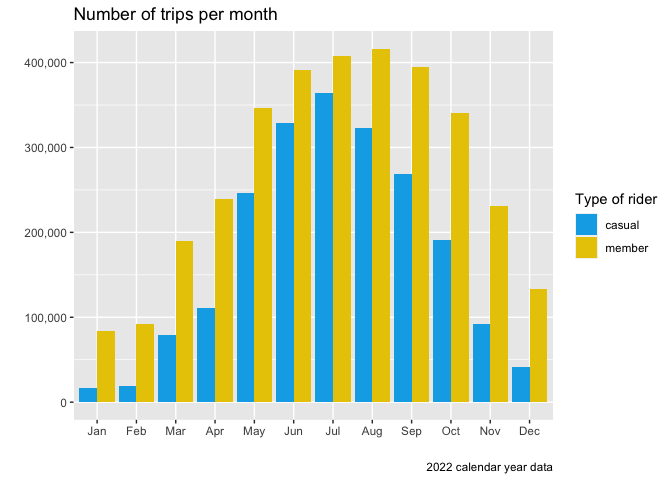
\includegraphics{CS_3_files/figure-latex/overall year load-1.pdf}

\begin{Shaded}
\begin{Highlighting}[]
\CommentTok{\# +}
\CommentTok{\#   geom\_text(aes(x = Month, y= count, label = count),}
\CommentTok{\#       hjust =0.5, vjust = 1.7, show.legend = FALSE, size = 2,}
\CommentTok{\#       position = position\_dodge(width = 1))}
\end{Highlighting}
\end{Shaded}

\begin{Shaded}
\begin{Highlighting}[]
\NormalTok{df }\SpecialCharTok{\%\textgreater{}\%} 
  \FunctionTok{filter}\NormalTok{(started\_at }\SpecialCharTok{\textless{}} \FunctionTok{ymd}\NormalTok{(}\StringTok{"2023{-}01{-}01"}\NormalTok{)) }\SpecialCharTok{\%\textgreater{}\%} \CommentTok{\# limit to a calendar year}
  \FunctionTok{group\_by}\NormalTok{(member\_casual, }\AttributeTok{Month=}  \FunctionTok{month}\NormalTok{(started\_at, }\AttributeTok{label =} \ConstantTok{TRUE}\NormalTok{)) }\SpecialCharTok{\%\textgreater{}\%}
  \FunctionTok{summarise}\NormalTok{(}\AttributeTok{count =} \FunctionTok{n}\NormalTok{()) }\SpecialCharTok{\%\textgreater{}\%}

  \FunctionTok{ggplot}\NormalTok{(}\FunctionTok{aes}\NormalTok{(}\AttributeTok{x =}\NormalTok{ Month, }\AttributeTok{y=}\NormalTok{ count, }\AttributeTok{fill =}\NormalTok{ member\_casual)) }\SpecialCharTok{+}
  \FunctionTok{geom\_col}\NormalTok{(}\AttributeTok{position =} \StringTok{"stack"}\NormalTok{) }\SpecialCharTok{+}
  \FunctionTok{labs}\NormalTok{(}\AttributeTok{title =} \StringTok{"Stacked Number of trips per month"}\NormalTok{,}
       \AttributeTok{caption =} \StringTok{"2022 calendar year data"}\NormalTok{,}
       \AttributeTok{x =}\StringTok{""}\NormalTok{, }\AttributeTok{y=} \StringTok{"Stacked count"}\NormalTok{,}
       \AttributeTok{fill=}\StringTok{\textquotesingle{}Type of rider\textquotesingle{}}\NormalTok{) }\SpecialCharTok{+}
  \FunctionTok{scale\_y\_continuous}\NormalTok{(}\AttributeTok{labels =} \FunctionTok{label\_comma}\NormalTok{()) }
\end{Highlighting}
\end{Shaded}

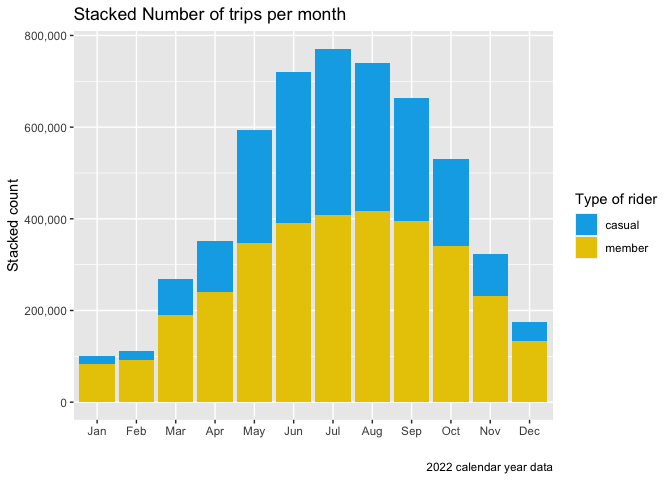
\includegraphics{CS_3_files/figure-latex/trips per month-1.pdf}

\begin{Shaded}
\begin{Highlighting}[]
\CommentTok{\# +}
\CommentTok{\#   geom\_text(aes(x = Month, y= count, label = count),}
\CommentTok{\#       hjust =0.5, vjust = 1.7, show.legend = FALSE, size = 2,}
\CommentTok{\#       position = position\_dodge(width = 1))}
\end{Highlighting}
\end{Shaded}

Insights:

\begin{itemize}
\item
  \textbf{Jan and Feb are the toughest month at Cyclistics}. The income
  is only \textasciitilde{} 16\% of year peaks.
\item
  \textbf{Members} generated \textbf{\textasciitilde80\% of income}
  during \textbf{Jan and Feb}.
\item
  In the summer months, the proportion begins to level off.
\end{itemize}

\hypertarget{average-trip-duration-by-day-of-week-month-rider}{%
\paragraph{Average trip duration by day of week, month,
rider}\label{average-trip-duration-by-day-of-week-month-rider}}

\begin{Shaded}
\begin{Highlighting}[]
\CommentTok{\# plotly interactive doesn\textquotesingle{}t work with github output}
\CommentTok{\# insp\_plt \textless{}{-}}
\NormalTok{df }\SpecialCharTok{\%\textgreater{}\%} 
  \FunctionTok{filter}\NormalTok{(started\_at }\SpecialCharTok{\textless{}} \FunctionTok{ymd}\NormalTok{(}\StringTok{"2023{-}01{-}01"}\NormalTok{)) }\SpecialCharTok{\%\textgreater{}\%} \CommentTok{\# limit to a calendar year}
  \FunctionTok{group\_by}\NormalTok{(member\_casual, }\AttributeTok{Month=}  \FunctionTok{month}\NormalTok{(started\_at, }\AttributeTok{label =} \ConstantTok{TRUE}\NormalTok{)) }\SpecialCharTok{\%\textgreater{}\%}
  \FunctionTok{summarise}\NormalTok{(}\AttributeTok{aver =} \FunctionTok{mean}\NormalTok{(trip\_duration)) }\SpecialCharTok{\%\textgreater{}\%}
  
  \FunctionTok{ggplot}\NormalTok{() }\SpecialCharTok{+}
  \FunctionTok{geom\_col}\NormalTok{(}\FunctionTok{aes}\NormalTok{(}\AttributeTok{x =}\NormalTok{ Month, }\AttributeTok{y=}\NormalTok{aver, }\AttributeTok{fill =}\NormalTok{ member\_casual),}
           \AttributeTok{position =} \StringTok{"dodge"}\NormalTok{, }\AttributeTok{alpha =} \DecValTok{1}\NormalTok{) }\SpecialCharTok{+}
  \FunctionTok{labs}\NormalTok{(}\AttributeTok{title =} \StringTok{"Average trip duration month by month"}\NormalTok{,}
       \AttributeTok{caption =}\NormalTok{ report\_caption,}
       \AttributeTok{x =}\StringTok{""}\NormalTok{, }\AttributeTok{y=} \StringTok{"Minutes"}\NormalTok{,}
       \AttributeTok{fill=}\StringTok{\textquotesingle{}Type of rider\textquotesingle{}}\NormalTok{) }\SpecialCharTok{+}
  \FunctionTok{scale\_y\_continuous}\NormalTok{(}\AttributeTok{labels =} \FunctionTok{label\_comma}\NormalTok{())}
\end{Highlighting}
\end{Shaded}

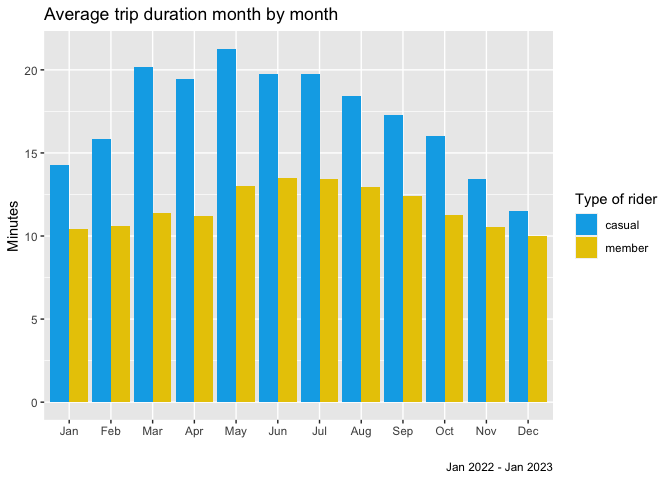
\includegraphics{CS_3_files/figure-latex/Monthly trip duration-1.pdf}

\begin{Shaded}
\begin{Highlighting}[]
\CommentTok{\# ggplotly(insp\_plt)}
\end{Highlighting}
\end{Shaded}

\hypertarget{number-of-trips-by-duration}{%
\paragraph{Number of trips by
duration}\label{number-of-trips-by-duration}}

\begin{Shaded}
\begin{Highlighting}[]
\NormalTok{df }\SpecialCharTok{\%\textgreater{}\%} 
  \FunctionTok{ggplot}\NormalTok{(}\FunctionTok{aes}\NormalTok{(}\AttributeTok{x =}\NormalTok{ trip\_duration, }\AttributeTok{fill =}\NormalTok{ member\_casual)) }\SpecialCharTok{+}
  \FunctionTok{geom\_histogram}\NormalTok{(}\AttributeTok{binwidth=} \DecValTok{5}\NormalTok{,}\AttributeTok{position =} \StringTok{"dodge"}\NormalTok{) }\SpecialCharTok{+} \CommentTok{\#}
  \FunctionTok{labs}\NormalTok{(}\AttributeTok{title =} \StringTok{"Trips by duration of ride"}\NormalTok{,}
       \AttributeTok{caption =} \StringTok{"Bin duration: 5 min"}\NormalTok{,}
       \AttributeTok{x =}\StringTok{"Minutes"}\NormalTok{, }\AttributeTok{y=} \StringTok{"Count of trips"}\NormalTok{,}
       \AttributeTok{fill=}\StringTok{\textquotesingle{}Type of rider\textquotesingle{}}\NormalTok{) }\SpecialCharTok{+}
  \FunctionTok{scale\_y\_continuous}\NormalTok{(}\AttributeTok{labels =} \FunctionTok{label\_comma}\NormalTok{())}\SpecialCharTok{+}
  \FunctionTok{xlim}\NormalTok{(}\DecValTok{0}\NormalTok{, }\DecValTok{65}\NormalTok{)}
\end{Highlighting}
\end{Shaded}

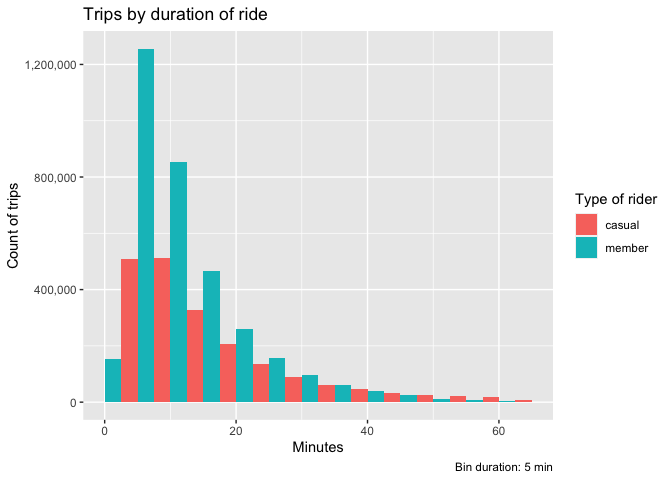
\includegraphics{CS_3_files/figure-latex/Trips by duration of ride-1.pdf}

Insights:

\begin{itemize}
\tightlist
\item
  Most trips (21\%) are made in the 5 to 15 minute range.
\end{itemize}

\begin{Shaded}
\begin{Highlighting}[]
\CommentTok{\# df \%\textgreater{}\% }
\CommentTok{\# summary(df$trip\_duration )}

\NormalTok{df }\SpecialCharTok{\%\textgreater{}\%} 
  \FunctionTok{mutate}\NormalTok{(}\AttributeTok{Month=}  \FunctionTok{month}\NormalTok{(started\_at, }\AttributeTok{label =} \ConstantTok{TRUE}\NormalTok{), }
         \AttributeTok{Ride\_duration =} \FunctionTok{round}\NormalTok{(trip\_duration)) }\SpecialCharTok{\%\textgreater{}\%} 

  \FunctionTok{crosstable}\NormalTok{(}\FunctionTok{c}\NormalTok{(}\StringTok{" "}\OtherTok{=}\NormalTok{Ride\_duration), }\AttributeTok{by=}\FunctionTok{c}\NormalTok{(}\StringTok{"Rider"} \OtherTok{=}\NormalTok{ member\_casual ), }\AttributeTok{funs =} \FunctionTok{c}\NormalTok{(mean, median), }\AttributeTok{total=}\StringTok{"both"}\NormalTok{, }\AttributeTok{showNA=}\StringTok{"no"}\NormalTok{, }
        \AttributeTok{percent\_digits=}\DecValTok{0}\NormalTok{, }\AttributeTok{percent\_pattern=}\StringTok{"\{n\} (\{p\_col\})"}\NormalTok{) }\SpecialCharTok{\%\textgreater{}\%} 
  \FunctionTok{as\_flextable}\NormalTok{(}\AttributeTok{compact=}\ConstantTok{TRUE}\NormalTok{, }\AttributeTok{keep\_id=}\ConstantTok{FALSE}\NormalTok{) }\SpecialCharTok{\%\textgreater{}\%} 
  \FunctionTok{set\_caption}\NormalTok{(}\FunctionTok{paste}\NormalTok{(}\StringTok{"Mean and median trip durations."}\NormalTok{, report\_caption))}
\end{Highlighting}
\end{Shaded}

\begin{verbatim}
## Warning: fonts used in `flextable` are ignored because the `pdflatex` engine is
## used and not `xelatex` or `lualatex`. You can avoid this warning by using the
## `set_flextable_defaults(fonts_ignore=TRUE)` command or use a compatible engine
## by defining `latex_engine: xelatex` in the YAML header of the R Markdown
## document.
\end{verbatim}

\global\setlength{\Oldarrayrulewidth}{\arrayrulewidth}

\global\setlength{\Oldtabcolsep}{\tabcolsep}

\setlength{\tabcolsep}{0pt}

\renewcommand*{\arraystretch}{1.5}



\providecommand{\ascline}[3]{\noalign{\global\arrayrulewidth #1}\arrayrulecolor[HTML]{#2}\cline{#3}}

\begin{longtable}[c]{|p{1.16in}|p{0.76in}|p{0.88in}|p{0.65in}}

\caption{Mean\ and\ median\ trip\ durations.\ Jan\ 2022\ -\ Jan\ 2023}\\

\ascline{1.5pt}{000000}{1-4}

\multicolumn{1}{>{\centering}m{\dimexpr 1.16in+0\tabcolsep}}{} & \multicolumn{2}{>{\centering}m{\dimexpr 1.64in+2\tabcolsep}}{\textcolor[HTML]{000000}{\fontsize{11}{11}\selectfont{\textbf{Rider}}}} & \multicolumn{1}{>{\centering}m{\dimexpr 0.65in+0\tabcolsep}}{} \\

\ascline{1pt}{000000}{2-3}



\multicolumn{1}{>{\centering}m{\dimexpr 1.16in+0\tabcolsep}}{\multirow[c]{-2}{*}{\parbox{1.16in}{\textcolor[HTML]{000000}{\fontsize{11}{11}\selectfont{\textbf{}}}}}} & \multicolumn{1}{>{\centering}m{\dimexpr 0.76in+0\tabcolsep}}{\textcolor[HTML]{000000}{\fontsize{11}{11}\selectfont{\textbf{casual}}}} & \multicolumn{1}{>{\centering}m{\dimexpr 0.88in+0\tabcolsep}}{\textcolor[HTML]{000000}{\fontsize{11}{11}\selectfont{\textbf{member}}}} & \multicolumn{1}{>{\centering}m{\dimexpr 0.65in+0\tabcolsep}}{\multirow[c]{-2}{*}{\parbox{0.65in}{\textcolor[HTML]{000000}{\fontsize{11}{11}\selectfont{\textbf{Total}}}}}} \\

\ascline{1.5pt}{000000}{1-4}\endhead



\multicolumn{1}{>{\raggedright}m{\dimexpr 1.16in+0\tabcolsep}}{\textcolor[HTML]{000000}{\fontsize{11}{11}\selectfont{\textbf{\ }}}} & \multicolumn{1}{>{\raggedright}m{\dimexpr 0.76in+0\tabcolsep}}{\textcolor[HTML]{000000}{\fontsize{11}{11}\selectfont{\textbf{}}}} & \multicolumn{1}{>{\raggedright}m{\dimexpr 0.88in+0\tabcolsep}}{\textcolor[HTML]{000000}{\fontsize{11}{11}\selectfont{}}} & \multicolumn{1}{>{\raggedright}m{\dimexpr 0.65in+0\tabcolsep}}{\textcolor[HTML]{000000}{\fontsize{11}{11}\selectfont{}}} \\





\multicolumn{1}{>{\raggedright}m{\dimexpr 1.16in+0\tabcolsep}}{\textcolor[HTML]{000000}{\fontsize{11}{11}\selectfont{mean}}} & \multicolumn{1}{>{\raggedright}m{\dimexpr 0.76in+0\tabcolsep}}{\textcolor[HTML]{000000}{\fontsize{11}{11}\selectfont{18.4}}} & \multicolumn{1}{>{\raggedright}m{\dimexpr 0.88in+0\tabcolsep}}{\textcolor[HTML]{000000}{\fontsize{11}{11}\selectfont{12.1}}} & \multicolumn{1}{>{\raggedright}m{\dimexpr 0.65in+0\tabcolsep}}{\textcolor[HTML]{000000}{\fontsize{11}{11}\selectfont{14.5}}} \\





\multicolumn{1}{>{\raggedright}m{\dimexpr 1.16in+0\tabcolsep}}{\textcolor[HTML]{000000}{\fontsize{11}{11}\selectfont{median}}} & \multicolumn{1}{>{\raggedright}m{\dimexpr 0.76in+0\tabcolsep}}{\textcolor[HTML]{000000}{\fontsize{11}{11}\selectfont{12.0}}} & \multicolumn{1}{>{\raggedright}m{\dimexpr 0.88in+0\tabcolsep}}{\textcolor[HTML]{000000}{\fontsize{11}{11}\selectfont{9.0}}} & \multicolumn{1}{>{\raggedright}m{\dimexpr 0.65in+0\tabcolsep}}{\textcolor[HTML]{000000}{\fontsize{11}{11}\selectfont{10.0}}} \\

\ascline{1.5pt}{666666}{1-4}



\end{longtable}



\arrayrulecolor[HTML]{000000}

\global\setlength{\arrayrulewidth}{\Oldarrayrulewidth}

\global\setlength{\tabcolsep}{\Oldtabcolsep}

\renewcommand*{\arraystretch}{1}

\hypertarget{share}{%
\subsection{5. SHARE}\label{share}}

Guiding questions:

\begin{enumerate}
\def\labelenumi{\arabic{enumi}.}
\item
  Were you able to answer the question of how annual members and casual
  riders use Cyclistic bikes differently?
\item
  What story does your data tell?
\item
  How do your findings relate to your original question?
\item
  Who is your audience? What is the best way to communicate with them?
\item
  Can data visualization help you share your findings?
\item
  Is your presentation accessible to your audience?
\end{enumerate}

\hypertarget{how-casual-riders-and-annual-members-use-cyclistic-bikes-differently}{%
\subsubsection{How casual riders and annual members use Cyclistic bikes
differently?}\label{how-casual-riders-and-annual-members-use-cyclistic-bikes-differently}}

We have figured out a significant differences in behaviour among
riders.\\
\textbf{Members} use Cyclistics to complete their daily activities, such
as commuting to work or school, running errands.\\
Members ride more often but their trips are shorter.\\
\textbf{Casual} riders most likely use bike share to explore Chicago,
get to appointments or social engagements, and more. And casual riders
prefer e-bikes.

\begin{longtable}[]{@{}
  >{\raggedright\arraybackslash}p{(\columnwidth - 4\tabcolsep) * \real{0.1957}}
  >{\raggedright\arraybackslash}p{(\columnwidth - 4\tabcolsep) * \real{0.3804}}
  >{\raggedright\arraybackslash}p{(\columnwidth - 4\tabcolsep) * \real{0.4185}}@{}}
\toprule()
\begin{minipage}[b]{\linewidth}\raggedright
\end{minipage} & \begin{minipage}[b]{\linewidth}\raggedright
members
\end{minipage} & \begin{minipage}[b]{\linewidth}\raggedright
casual riders
\end{minipage} \\
\midrule()
\endhead
\begin{minipage}[t]{\linewidth}\raggedright
number of trips\\
min-max per month\strut
\end{minipage} & \begin{minipage}[t]{\linewidth}\raggedright
\hfill\break
83482 - 416457\strut
\end{minipage} & \begin{minipage}[t]{\linewidth}\raggedright
\hfill\break
16997 - 363992\strut
\end{minipage} \\
spread of trip duration per month &
\begin{minipage}[t]{\linewidth}\raggedright
10-13 min\\
(Dec-Jun)\strut
\end{minipage} & \begin{minipage}[t]{\linewidth}\raggedright
12-22 min\\
(Dec-May)\strut
\end{minipage} \\
year average trip duration & 12.1 & 18,4 \\
mode of day of week & Tue, Wed, Thu & Sat \\
anti-mode of day of week & Sun & Mon-Tue \\
bike type preference & doesn't matter & e-bike \\
weather dependence & medium & high \\
\begin{minipage}[t]{\linewidth}\raggedright
seasonal patterns\\
Jan -Jul rides\strut
\end{minipage} & \begin{minipage}[t]{\linewidth}\raggedright
medium\\
1:5\strut
\end{minipage} & \begin{minipage}[t]{\linewidth}\raggedright
very high\\
1:21\strut
\end{minipage} \\
\textbf{most likely purpose of use} & \textbf{commute to work or school,
run errands, performing daily duties} & \textbf{explore Chicago, get to
appointments or social engagements on weekends} \\
\bottomrule()
\end{longtable}

\hypertarget{why-would-casual-riders-buy-cyclistic-annual-memberships}{%
\subsubsection{Why would casual riders buy Cyclistic annual
memberships?}\label{why-would-casual-riders-buy-cyclistic-annual-memberships}}

So, how can we steer casual riders to became a Cyclistics member?\\
We should accent our offerings on the preferences that have been figured
out in the report. It means we should include special e-bikes proposal
into annual membership.

\begin{enumerate}
\def\labelenumi{\arabic{enumi}.}
\item
  Annual \textbf{prime membership} which includes 30-45 minutes of
  e-bike rides a day.\\
  The price should be higher than ordinary membership, say 175-200 \$
  but\\
  Additional research should be conducted about specific pricing
  parameters.
\item
  Customers may consider to buy personal e-bikes, but we should launch
  \textbf{an awareness campaign} about the benefits of e-bike sharing
  (charging, service, does not take up space in the apartment, not have
  to worry a single second about a bike being stolen, etc.)
\item
  Investigate most popular casual riders routes in Chicago and inform
  potential customers about future locations of dock stations. Conduct a
  survey among potential customers where to locate stations.
\end{enumerate}

Let's don't forget about our current customers. New proposal shouldn't
contradict their current membership (accent on classic bike usage).

\hypertarget{how-can-cyclistic-use-digital-media-to-influence-casual-riders-to-become-members}{%
\subsubsection{How can Cyclistic use digital media to influence casual
riders to become
members?}\label{how-can-cyclistic-use-digital-media-to-influence-casual-riders-to-become-members}}

\begin{enumerate}
\def\labelenumi{\arabic{enumi}.}
\item
  Use social networks to populate bike sharing.
\item
  Use direct targeting on potential customers. Send direct proposals
  using mobile app every customers have already installed.
\item
  Collaboration with local parks and attractions to populate bike using.
  Invest into popular bike apps like Komoot, Strava to inform local
  customers about Cyclistics.
\end{enumerate}

\hypertarget{act}{%
\subsection{6. ACT}\label{act}}

\begin{enumerate}
\def\labelenumi{\arabic{enumi}.}
\item
  What is your final conclusion based on your analysis?\\
  Casual riders are not avid bikers. The are ready to pay more for
  e-bike rent.\\
  We have to make them an offer from which they are unlikely to refuse.
\item
  How could your team and business apply your insights?\\
  We need to develop a marketing campaign to promote e-bikes rent among
  members.
\item
  What next steps would you or your stakeholders take based on your
  findings?\\
  Invest time and efforts into additional exploration of potential
  customers and their needs, polishing special proposals among customers
  segments.
\item
  Is there additional data you could use to expand on your findings?\\
  Add Boston 2022 weather (temperature, precipitation)\\
  Add viz with geo data most pop stations\\
  Define a correlation member\_casual - weather conditions.
\end{enumerate}

Additional work:

\begin{enumerate}
\def\labelenumi{\arabic{enumi}.}
\item
  Add Boston 2022 weather (temperature, precipitation)
\item
  add viz with geo data most pop stations
\item
  correlation member\_casual - weather conditions.
\end{enumerate}

\begin{Shaded}
\begin{Highlighting}[]
\CommentTok{\# geo\_df \textless{}{-}}
\CommentTok{\# stations\_df \%\textgreater{}\% }
  \CommentTok{\# filter(end\_lng2 \textless{} {-}87)}
\end{Highlighting}
\end{Shaded}

\begin{Shaded}
\begin{Highlighting}[]
\CommentTok{\# chi\_map \textless{}{-} read\_sf("https://raw.githubusercontent.com/thisisdaryn/data/master/geo/chicago/Comm\_Areas.geojson")}

  \CommentTok{\# ggplot(chi\_map) +}
  \CommentTok{\# geom\_sf() + }
  \CommentTok{\# geom\_point(data = geo\_df, mapping = aes(x = end\_lng2, y = end\_lat2),}
  \CommentTok{\#            size = 1, stroke = 0, color = "red") +}
  \CommentTok{\# geom\_text(data = geo\_df, aes(x=end\_lng2, y=end\_lat2, label=station\_name),}
  \CommentTok{\#           size = 3,  check\_overlap = TRUE, color= "blue") \# hjust=0, vjust={-}1,}
\end{Highlighting}
\end{Shaded}

\begin{Shaded}
\begin{Highlighting}[]
\CommentTok{\# insp\_plt \textless{}{-} ggplot(data = chi\_map) + }
\CommentTok{\#   geom\_sf() +}
\CommentTok{\#   geom\_point(data = geo\_df, }
\CommentTok{\#              aes(x = end\_lng2, y = end\_lat2, }
\CommentTok{\#                  colour = "red"))  \# , label=station\_name}
\CommentTok{\# ggplotly(insp\_plt)}
\end{Highlighting}
\end{Shaded}


\end{document}
